% Options for packages loaded elsewhere
\PassOptionsToPackage{unicode}{hyperref}
\PassOptionsToPackage{hyphens}{url}
\PassOptionsToPackage{dvipsnames,svgnames,x11names}{xcolor}
%
\documentclass[
  letterpaper,
  DIV=11,
  numbers=noendperiod]{scrartcl}

\usepackage{amsmath,amssymb}
\usepackage{iftex}
\ifPDFTeX
  \usepackage[T1]{fontenc}
  \usepackage[utf8]{inputenc}
  \usepackage{textcomp} % provide euro and other symbols
\else % if luatex or xetex
  \usepackage{unicode-math}
  \defaultfontfeatures{Scale=MatchLowercase}
  \defaultfontfeatures[\rmfamily]{Ligatures=TeX,Scale=1}
\fi
\usepackage{lmodern}
\ifPDFTeX\else  
    % xetex/luatex font selection
\fi
% Use upquote if available, for straight quotes in verbatim environments
\IfFileExists{upquote.sty}{\usepackage{upquote}}{}
\IfFileExists{microtype.sty}{% use microtype if available
  \usepackage[]{microtype}
  \UseMicrotypeSet[protrusion]{basicmath} % disable protrusion for tt fonts
}{}
\makeatletter
\@ifundefined{KOMAClassName}{% if non-KOMA class
  \IfFileExists{parskip.sty}{%
    \usepackage{parskip}
  }{% else
    \setlength{\parindent}{0pt}
    \setlength{\parskip}{6pt plus 2pt minus 1pt}}
}{% if KOMA class
  \KOMAoptions{parskip=half}}
\makeatother
\usepackage{xcolor}
\setlength{\emergencystretch}{3em} % prevent overfull lines
\setcounter{secnumdepth}{-\maxdimen} % remove section numbering
% Make \paragraph and \subparagraph free-standing
\ifx\paragraph\undefined\else
  \let\oldparagraph\paragraph
  \renewcommand{\paragraph}[1]{\oldparagraph{#1}\mbox{}}
\fi
\ifx\subparagraph\undefined\else
  \let\oldsubparagraph\subparagraph
  \renewcommand{\subparagraph}[1]{\oldsubparagraph{#1}\mbox{}}
\fi

\usepackage{color}
\usepackage{fancyvrb}
\newcommand{\VerbBar}{|}
\newcommand{\VERB}{\Verb[commandchars=\\\{\}]}
\DefineVerbatimEnvironment{Highlighting}{Verbatim}{commandchars=\\\{\}}
% Add ',fontsize=\small' for more characters per line
\usepackage{framed}
\definecolor{shadecolor}{RGB}{241,243,245}
\newenvironment{Shaded}{\begin{snugshade}}{\end{snugshade}}
\newcommand{\AlertTok}[1]{\textcolor[rgb]{0.68,0.00,0.00}{#1}}
\newcommand{\AnnotationTok}[1]{\textcolor[rgb]{0.37,0.37,0.37}{#1}}
\newcommand{\AttributeTok}[1]{\textcolor[rgb]{0.40,0.45,0.13}{#1}}
\newcommand{\BaseNTok}[1]{\textcolor[rgb]{0.68,0.00,0.00}{#1}}
\newcommand{\BuiltInTok}[1]{\textcolor[rgb]{0.00,0.23,0.31}{#1}}
\newcommand{\CharTok}[1]{\textcolor[rgb]{0.13,0.47,0.30}{#1}}
\newcommand{\CommentTok}[1]{\textcolor[rgb]{0.37,0.37,0.37}{#1}}
\newcommand{\CommentVarTok}[1]{\textcolor[rgb]{0.37,0.37,0.37}{\textit{#1}}}
\newcommand{\ConstantTok}[1]{\textcolor[rgb]{0.56,0.35,0.01}{#1}}
\newcommand{\ControlFlowTok}[1]{\textcolor[rgb]{0.00,0.23,0.31}{#1}}
\newcommand{\DataTypeTok}[1]{\textcolor[rgb]{0.68,0.00,0.00}{#1}}
\newcommand{\DecValTok}[1]{\textcolor[rgb]{0.68,0.00,0.00}{#1}}
\newcommand{\DocumentationTok}[1]{\textcolor[rgb]{0.37,0.37,0.37}{\textit{#1}}}
\newcommand{\ErrorTok}[1]{\textcolor[rgb]{0.68,0.00,0.00}{#1}}
\newcommand{\ExtensionTok}[1]{\textcolor[rgb]{0.00,0.23,0.31}{#1}}
\newcommand{\FloatTok}[1]{\textcolor[rgb]{0.68,0.00,0.00}{#1}}
\newcommand{\FunctionTok}[1]{\textcolor[rgb]{0.28,0.35,0.67}{#1}}
\newcommand{\ImportTok}[1]{\textcolor[rgb]{0.00,0.46,0.62}{#1}}
\newcommand{\InformationTok}[1]{\textcolor[rgb]{0.37,0.37,0.37}{#1}}
\newcommand{\KeywordTok}[1]{\textcolor[rgb]{0.00,0.23,0.31}{#1}}
\newcommand{\NormalTok}[1]{\textcolor[rgb]{0.00,0.23,0.31}{#1}}
\newcommand{\OperatorTok}[1]{\textcolor[rgb]{0.37,0.37,0.37}{#1}}
\newcommand{\OtherTok}[1]{\textcolor[rgb]{0.00,0.23,0.31}{#1}}
\newcommand{\PreprocessorTok}[1]{\textcolor[rgb]{0.68,0.00,0.00}{#1}}
\newcommand{\RegionMarkerTok}[1]{\textcolor[rgb]{0.00,0.23,0.31}{#1}}
\newcommand{\SpecialCharTok}[1]{\textcolor[rgb]{0.37,0.37,0.37}{#1}}
\newcommand{\SpecialStringTok}[1]{\textcolor[rgb]{0.13,0.47,0.30}{#1}}
\newcommand{\StringTok}[1]{\textcolor[rgb]{0.13,0.47,0.30}{#1}}
\newcommand{\VariableTok}[1]{\textcolor[rgb]{0.07,0.07,0.07}{#1}}
\newcommand{\VerbatimStringTok}[1]{\textcolor[rgb]{0.13,0.47,0.30}{#1}}
\newcommand{\WarningTok}[1]{\textcolor[rgb]{0.37,0.37,0.37}{\textit{#1}}}

\providecommand{\tightlist}{%
  \setlength{\itemsep}{0pt}\setlength{\parskip}{0pt}}\usepackage{longtable,booktabs,array}
\usepackage{calc} % for calculating minipage widths
% Correct order of tables after \paragraph or \subparagraph
\usepackage{etoolbox}
\makeatletter
\patchcmd\longtable{\par}{\if@noskipsec\mbox{}\fi\par}{}{}
\makeatother
% Allow footnotes in longtable head/foot
\IfFileExists{footnotehyper.sty}{\usepackage{footnotehyper}}{\usepackage{footnote}}
\makesavenoteenv{longtable}
\usepackage{graphicx}
\makeatletter
\def\maxwidth{\ifdim\Gin@nat@width>\linewidth\linewidth\else\Gin@nat@width\fi}
\def\maxheight{\ifdim\Gin@nat@height>\textheight\textheight\else\Gin@nat@height\fi}
\makeatother
% Scale images if necessary, so that they will not overflow the page
% margins by default, and it is still possible to overwrite the defaults
% using explicit options in \includegraphics[width, height, ...]{}
\setkeys{Gin}{width=\maxwidth,height=\maxheight,keepaspectratio}
% Set default figure placement to htbp
\makeatletter
\def\fps@figure{htbp}
\makeatother

\usepackage{float}
\usepackage{tabularray}
\usepackage[normalem]{ulem}
\usepackage{graphicx}
\UseTblrLibrary{booktabs}
\UseTblrLibrary{siunitx}
\NewTableCommand{\tinytableDefineColor}[3]{\definecolor{#1}{#2}{#3}}
\newcommand{\tinytableTabularrayUnderline}[1]{\underline{#1}}
\newcommand{\tinytableTabularrayStrikeout}[1]{\sout{#1}}
\KOMAoption{captions}{tableheading}
\makeatletter
\@ifpackageloaded{caption}{}{\usepackage{caption}}
\AtBeginDocument{%
\ifdefined\contentsname
  \renewcommand*\contentsname{Table of contents}
\else
  \newcommand\contentsname{Table of contents}
\fi
\ifdefined\listfigurename
  \renewcommand*\listfigurename{List of Figures}
\else
  \newcommand\listfigurename{List of Figures}
\fi
\ifdefined\listtablename
  \renewcommand*\listtablename{List of Tables}
\else
  \newcommand\listtablename{List of Tables}
\fi
\ifdefined\figurename
  \renewcommand*\figurename{Figure}
\else
  \newcommand\figurename{Figure}
\fi
\ifdefined\tablename
  \renewcommand*\tablename{Table}
\else
  \newcommand\tablename{Table}
\fi
}
\@ifpackageloaded{float}{}{\usepackage{float}}
\floatstyle{ruled}
\@ifundefined{c@chapter}{\newfloat{codelisting}{h}{lop}}{\newfloat{codelisting}{h}{lop}[chapter]}
\floatname{codelisting}{Listing}
\newcommand*\listoflistings{\listof{codelisting}{List of Listings}}
\makeatother
\makeatletter
\makeatother
\makeatletter
\@ifpackageloaded{caption}{}{\usepackage{caption}}
\@ifpackageloaded{subcaption}{}{\usepackage{subcaption}}
\makeatother
\ifLuaTeX
  \usepackage{selnolig}  % disable illegal ligatures
\fi
\usepackage{bookmark}

\IfFileExists{xurl.sty}{\usepackage{xurl}}{} % add URL line breaks if available
\urlstyle{same} % disable monospaced font for URLs
\hypersetup{
  pdftitle={TCC},
  pdfauthor={Victor Alves},
  colorlinks=true,
  linkcolor={blue},
  filecolor={Maroon},
  citecolor={Blue},
  urlcolor={Blue},
  pdfcreator={LaTeX via pandoc}}

\title{TCC}
\author{Victor Alves}
\date{}

\begin{document}
\maketitle

\section{Loading Packages}\label{loading-packages}

\begin{Shaded}
\begin{Highlighting}[]
\CommentTok{\# Carrega os pacotes necessários para a análise de dados}
\FunctionTok{library}\NormalTok{(tidyverse)    }\CommentTok{\# Pacote que inclui uma coleção de pacotes para manipulação, }
\CommentTok{\#visualização e modelagem de dados.}
\FunctionTok{library}\NormalTok{(did) }\CommentTok{\# Pacote criado por Callway \& Sant\textquotesingle{}Anna (2022) para seu método de DiD}
\FunctionTok{library}\NormalTok{(bacondecomp)}
\FunctionTok{library}\NormalTok{(geobr) }\CommentTok{\# Pacote para trabalhar com gráficos de mapa do Brasil}
\FunctionTok{library}\NormalTok{(magrittr)     }\CommentTok{\# Pacote que permite escrever códigos mais legíveis e }
\CommentTok{\#organizados utilizando o operador \%\textgreater{}\%}
\FunctionTok{library}\NormalTok{(lubridate)    }\CommentTok{\# Pacote para trabalhar com datas}
\FunctionTok{library}\NormalTok{(zoo)          }\CommentTok{\# Pacote para trabalhar com séries temporais}
\FunctionTok{library}\NormalTok{(janitor)      }\CommentTok{\# Pacote para limpeza e transformação de dados}
\FunctionTok{library}\NormalTok{(readxl)       }\CommentTok{\# Pacote para importar dados de arquivos do Excel}
\FunctionTok{library}\NormalTok{(stargazer)    }\CommentTok{\# Pacote para criar tabelas de resultados de modelos}
\FunctionTok{library}\NormalTok{(ggthemes)     }\CommentTok{\# Pacote para personalização de gráficos criados com ggplot2}
\FunctionTok{library}\NormalTok{(viridis)      }\CommentTok{\# Pacote para gerar paletas de cores para gráficos}
\FunctionTok{library}\NormalTok{(GGally)       }\CommentTok{\# Pacote para criação de matriz de dispersão}
\FunctionTok{library}\NormalTok{(gridExtra)    }\CommentTok{\# Pacote para combinar vários gráficos em uma única imagem}
\FunctionTok{library}\NormalTok{(grid)         }\CommentTok{\# Pacote para trabalhar com layout e alinhamento de gráficos}
\FunctionTok{library}\NormalTok{(gridtext)     }\CommentTok{\# Pacote para adicionar texto em gráficos gerados com grid}
\FunctionTok{library}\NormalTok{(plm)          }\CommentTok{\# Pacote para modelagem de dados em painel}
\FunctionTok{library}\NormalTok{(tempdisagg)   }\CommentTok{\# Pacote para desagregação temporal de séries de tempo}
\FunctionTok{library}\NormalTok{(showtext)     }\CommentTok{\# Pacote de fontes}
\FunctionTok{library}\NormalTok{(forecast)     }\CommentTok{\# Pacote para séries temporais}
\FunctionTok{library}\NormalTok{(broom)}
\FunctionTok{library}\NormalTok{(xtable)}
\FunctionTok{library}\NormalTok{(modelsummary)}
\FunctionTok{library}\NormalTok{(gt)}
\end{Highlighting}
\end{Shaded}

\section{Data}\label{data}

\subsection{Loading data}\label{loading-data}

\subsubsection{Loading original data}\label{loading-original-data}

\begin{Shaded}
\begin{Highlighting}[]
\FunctionTok{setwd}\NormalTok{(}\StringTok{"G:/Meu Drive/Insper/TCC"}\NormalTok{)}

\NormalTok{dados\_ice\_v3 }\OtherTok{\textless{}{-}}\NormalTok{ arrow}\SpecialCharTok{::}\FunctionTok{read\_parquet}\NormalTok{(}\StringTok{\textquotesingle{}Dados/dados\_ice\_v3\_limpo.parquet\textquotesingle{}}\NormalTok{) }\SpecialCharTok{\%\textgreater{}\%} 
  \FunctionTok{filter}\NormalTok{(ano\_enem }\SpecialCharTok{\textgreater{}=} \DecValTok{2009}\NormalTok{) }\SpecialCharTok{\%\textgreater{}\%} 
  \FunctionTok{mutate}\NormalTok{(}\AttributeTok{cod\_munic =} \FunctionTok{as.numeric}\NormalTok{(cod\_munic))}

\NormalTok{painel\_indicadores }\OtherTok{\textless{}{-}}\NormalTok{ arrow}\SpecialCharTok{::}\FunctionTok{read\_parquet}\NormalTok{(}\StringTok{\textquotesingle{}Dados/painel\_indicadores.parquet\textquotesingle{}}\NormalTok{)}

\NormalTok{painel\_indicadores\_simplificado }\OtherTok{\textless{}{-}}\NormalTok{ arrow}\SpecialCharTok{::}\FunctionTok{read\_parquet}\NormalTok{(}\StringTok{\textquotesingle{}Dados/painel\_indicadores\_simplificado.parquet\textquotesingle{}}\NormalTok{)}
\end{Highlighting}
\end{Shaded}

\begin{Shaded}
\begin{Highlighting}[]
\NormalTok{dados\_ice\_v3\_norm }\OtherTok{\textless{}{-}}\NormalTok{ dados\_ice\_v3 }\SpecialCharTok{\%\textgreater{}\%} 
  \FunctionTok{mutate\_at}\NormalTok{(}\FunctionTok{c}\NormalTok{(}\StringTok{\textquotesingle{}enem\_nota\_objetiva\textquotesingle{}}\NormalTok{,}\StringTok{\textquotesingle{}enem\_nota\_redacao\textquotesingle{}}\NormalTok{, }\StringTok{\textquotesingle{}enem\_nota\_matematica\textquotesingle{}}\NormalTok{, }\StringTok{\textquotesingle{}enem\_nota\_linguagens\textquotesingle{}}\NormalTok{,}
              \StringTok{\textquotesingle{}enem\_nota\_humanas\textquotesingle{}}\NormalTok{, }\StringTok{\textquotesingle{}enem\_nota\_humanas\textquotesingle{}}\NormalTok{, }\StringTok{\textquotesingle{}enem\_nota\_ciencias\textquotesingle{}}\NormalTok{, }\StringTok{\textquotesingle{}enem\_nota\_objetivab\textquotesingle{}}\NormalTok{), }
            \SpecialCharTok{\textasciitilde{}}\NormalTok{(}\FunctionTok{scale}\NormalTok{(.) }\SpecialCharTok{\%\textgreater{}\%}\NormalTok{ as.vector))}

\NormalTok{painel\_indicadores\_simplificado\_norm }\OtherTok{\textless{}{-}}\NormalTok{ painel\_indicadores\_simplificado }\SpecialCharTok{\%\textgreater{}\%} 
  \FunctionTok{mutate\_at}\NormalTok{(}\FunctionTok{c}\NormalTok{(}\StringTok{\textquotesingle{}aba\_em\textquotesingle{}}\NormalTok{, }\StringTok{\textquotesingle{}dist\_em\textquotesingle{}}\NormalTok{, }\StringTok{\textquotesingle{}apr\_em\textquotesingle{}}\NormalTok{, }\StringTok{\textquotesingle{}rep\_em\textquotesingle{}}\NormalTok{),  }\SpecialCharTok{\textasciitilde{}}\NormalTok{(}\FunctionTok{scale}\NormalTok{(.) }\SpecialCharTok{\%\textgreater{}\%}\NormalTok{ as.vector))}
\end{Highlighting}
\end{Shaded}

\begin{Shaded}
\begin{Highlighting}[]
\NormalTok{tema }\OtherTok{\textless{}{-}} \FunctionTok{theme}\NormalTok{(}\AttributeTok{plot.title =} \FunctionTok{element\_text}\NormalTok{(}\AttributeTok{size =} \DecValTok{16}\NormalTok{, }\AttributeTok{face =} \StringTok{"bold"}\NormalTok{, }\AttributeTok{hjust =} \FloatTok{0.5}\NormalTok{),}
              \AttributeTok{axis.line =} \FunctionTok{element\_line}\NormalTok{(}\AttributeTok{colour =} \StringTok{"black"}\NormalTok{),}
              \AttributeTok{axis.text.y =} \FunctionTok{element\_text}\NormalTok{(}\AttributeTok{angle =} \DecValTok{0}\NormalTok{, }\AttributeTok{size =} \DecValTok{12}\NormalTok{, }\AttributeTok{face =} \StringTok{\textquotesingle{}plain\textquotesingle{}}\NormalTok{),}
              \AttributeTok{axis.text.x =} \FunctionTok{element\_text}\NormalTok{(}\AttributeTok{angle =} \DecValTok{90}\NormalTok{, }\AttributeTok{size =} \DecValTok{12}\NormalTok{, }\AttributeTok{face =} \StringTok{\textquotesingle{}plain\textquotesingle{}}\NormalTok{),}
              \AttributeTok{axis.title =} \FunctionTok{element\_text}\NormalTok{(}\AttributeTok{size =} \DecValTok{14}\NormalTok{, }\AttributeTok{face =} \StringTok{\textquotesingle{}plain\textquotesingle{}}\NormalTok{),}
              \AttributeTok{legend.title =} \FunctionTok{element\_text}\NormalTok{(}\AttributeTok{size =} \DecValTok{10}\NormalTok{),}
              \AttributeTok{legend.text =} \FunctionTok{element\_text}\NormalTok{(}\AttributeTok{size =} \DecValTok{10}\NormalTok{),}
              \AttributeTok{plot.background =} \FunctionTok{element\_rect}\NormalTok{(}\AttributeTok{fill =} \FunctionTok{alpha}\NormalTok{(}\StringTok{"white"}\NormalTok{, }\FloatTok{0.25}\NormalTok{), }
                                       \AttributeTok{color =} \ConstantTok{NA}\NormalTok{),}
              \AttributeTok{legend.background =} \FunctionTok{element\_rect}\NormalTok{(}\AttributeTok{fill =} \StringTok{"transparent"}\NormalTok{, }\AttributeTok{color =} \ConstantTok{NA}\NormalTok{))}

\NormalTok{tema\_did }\OtherTok{\textless{}{-}} \FunctionTok{theme}\NormalTok{(}\AttributeTok{plot.title =} \FunctionTok{element\_text}\NormalTok{(}\AttributeTok{size =} \DecValTok{16}\NormalTok{, }\AttributeTok{face =} \StringTok{"bold"}\NormalTok{, }\AttributeTok{hjust =} \FloatTok{0.5}\NormalTok{),}
              \AttributeTok{legend.text =} \FunctionTok{element\_text}\NormalTok{(}\AttributeTok{size =} \DecValTok{16}\NormalTok{),}
              \AttributeTok{axis.line =} \FunctionTok{element\_line}\NormalTok{(}\AttributeTok{colour =} \StringTok{"black"}\NormalTok{),}
              \AttributeTok{axis.text.y =} \FunctionTok{element\_text}\NormalTok{(}\AttributeTok{angle =} \DecValTok{0}\NormalTok{, }\AttributeTok{size =} \DecValTok{14}\NormalTok{, }\AttributeTok{face =} \StringTok{\textquotesingle{}plain\textquotesingle{}}\NormalTok{),}
              \AttributeTok{axis.text.x =} \FunctionTok{element\_text}\NormalTok{(}\AttributeTok{angle =} \DecValTok{0}\NormalTok{, }\AttributeTok{size =} \DecValTok{14}\NormalTok{, }\AttributeTok{face =} \StringTok{\textquotesingle{}plain\textquotesingle{}}\NormalTok{),}
              \AttributeTok{axis.title =} \FunctionTok{element\_text}\NormalTok{(}\AttributeTok{size =} \DecValTok{14}\NormalTok{, }\AttributeTok{face =} \StringTok{\textquotesingle{}plain\textquotesingle{}}\NormalTok{),}
              \AttributeTok{legend.title =} \FunctionTok{element\_text}\NormalTok{(}\AttributeTok{size =} \DecValTok{10}\NormalTok{),}
              \AttributeTok{plot.background =} \FunctionTok{element\_rect}\NormalTok{(}\AttributeTok{fill =} \FunctionTok{alpha}\NormalTok{(}\StringTok{"white"}\NormalTok{, }\FloatTok{0.25}\NormalTok{), }
                                       \AttributeTok{color =} \ConstantTok{NA}\NormalTok{),}
              \AttributeTok{panel.background =} \FunctionTok{element\_rect}\NormalTok{(}\AttributeTok{fill =} \StringTok{"transparent"}\NormalTok{, }\AttributeTok{color =} \ConstantTok{NA}\NormalTok{),}
              \AttributeTok{legend.background =} \FunctionTok{element\_rect}\NormalTok{(}\AttributeTok{fill =} \StringTok{"transparent"}\NormalTok{, }\AttributeTok{color =} \ConstantTok{NA}\NormalTok{))}
\end{Highlighting}
\end{Shaded}

\section{Descriptives}\label{descriptives}

\begin{Shaded}
\begin{Highlighting}[]
\NormalTok{dados\_ice\_v3 }\SpecialCharTok{\%\textgreater{}\%} 
  \FunctionTok{filter}\NormalTok{(ano\_enem }\SpecialCharTok{\textgreater{}=} \DecValTok{2009}\NormalTok{) }\SpecialCharTok{\%\textgreater{}\%} 
    \FunctionTok{mutate}\NormalTok{(}\AttributeTok{ano\_enem =}\NormalTok{ lubridate}\SpecialCharTok{::}\FunctionTok{ymd}\NormalTok{(ano\_enem, }\AttributeTok{truncated =} \DecValTok{2}\NormalTok{L),}
           \AttributeTok{tratado =} \FunctionTok{as\_factor}\NormalTok{(tratado),}
           \AttributeTok{tratado =} \FunctionTok{case\_when}\NormalTok{(tratado }\SpecialCharTok{==} \DecValTok{1} \SpecialCharTok{\textasciitilde{}} \StringTok{"Possui EMI"}\NormalTok{,}
\NormalTok{                               tratado }\SpecialCharTok{!=} \DecValTok{1} \SpecialCharTok{\textasciitilde{}} \StringTok{"Não possui EMI"}\NormalTok{,}
\NormalTok{                               T }\SpecialCharTok{\textasciitilde{}}\NormalTok{ tratado)) }\SpecialCharTok{\%\textgreater{}\%}
    \FunctionTok{group\_by}\NormalTok{(ano\_enem, tratado) }\SpecialCharTok{\%\textgreater{}\%} 
    \FunctionTok{summarise}\NormalTok{(}\AttributeTok{enem\_nota\_redacao =} \FunctionTok{mean}\NormalTok{(enem\_nota\_redacao, }\AttributeTok{na.rm =}\NormalTok{ T),}
              \AttributeTok{enem\_nota\_matematica =} \FunctionTok{mean}\NormalTok{(enem\_nota\_matematica, }\AttributeTok{na.rm =}\NormalTok{ T),}
              \AttributeTok{enem\_nota\_linguagens =} \FunctionTok{mean}\NormalTok{(enem\_nota\_linguagens, }\AttributeTok{na.rm =}\NormalTok{ T),}
              \AttributeTok{enem\_nota\_ciencias =} \FunctionTok{mean}\NormalTok{(enem\_nota\_ciencias, }\AttributeTok{na.rm =}\NormalTok{ T),}
              \AttributeTok{enem\_nota\_humanas =} \FunctionTok{mean}\NormalTok{(enem\_nota\_humanas, }\AttributeTok{na.rm =}\NormalTok{ T)}
\NormalTok{              ) }\SpecialCharTok{\%\textgreater{}\%}
  \FunctionTok{pivot\_longer}\NormalTok{(}\SpecialCharTok{!}\FunctionTok{c}\NormalTok{(ano\_enem, tratado), }
               \AttributeTok{names\_to =} \StringTok{\textquotesingle{}prova\textquotesingle{}}\NormalTok{,}
               \AttributeTok{values\_to =} \StringTok{\textquotesingle{}nota\textquotesingle{}}\NormalTok{) }\SpecialCharTok{\%\textgreater{}\%} 
  \FunctionTok{mutate}\NormalTok{(}\AttributeTok{prova =} \FunctionTok{case\_when}\NormalTok{(prova }\SpecialCharTok{==} \StringTok{\textquotesingle{}enem\_nota\_redacao\textquotesingle{}} \SpecialCharTok{\textasciitilde{}} \StringTok{\textquotesingle{}Redação\textquotesingle{}}\NormalTok{,}
\NormalTok{                           prova }\SpecialCharTok{==} \StringTok{\textquotesingle{}enem\_nota\_matematica\textquotesingle{}} \SpecialCharTok{\textasciitilde{}} \StringTok{\textquotesingle{}Matemática\textquotesingle{}}\NormalTok{,}
\NormalTok{                           prova }\SpecialCharTok{==} \StringTok{\textquotesingle{}enem\_nota\_linguagens\textquotesingle{}} \SpecialCharTok{\textasciitilde{}} \StringTok{\textquotesingle{}Linguagens\textquotesingle{}}\NormalTok{,}
\NormalTok{                           prova }\SpecialCharTok{==} \StringTok{\textquotesingle{}enem\_nota\_humanas\textquotesingle{}} \SpecialCharTok{\textasciitilde{}} \StringTok{\textquotesingle{}Ciências Humanas\textquotesingle{}}\NormalTok{,}
\NormalTok{                           prova }\SpecialCharTok{==} \StringTok{\textquotesingle{}enem\_nota\_ciencias\textquotesingle{}} \SpecialCharTok{\textasciitilde{}} \StringTok{\textquotesingle{}Ciências Naturais\textquotesingle{}}\NormalTok{,}
\NormalTok{                           T }\SpecialCharTok{\textasciitilde{}}\NormalTok{ prova)) }\SpecialCharTok{\%\textgreater{}\%} 
  \FunctionTok{ggplot}\NormalTok{() }\SpecialCharTok{+}
  \FunctionTok{geom\_point}\NormalTok{(}\FunctionTok{aes}\NormalTok{(ano\_enem, nota, }\AttributeTok{colour =}\NormalTok{ tratado)) }\SpecialCharTok{+}
  \FunctionTok{geom\_line}\NormalTok{(}\FunctionTok{aes}\NormalTok{(ano\_enem, nota, }\AttributeTok{colour =}\NormalTok{ tratado)) }\SpecialCharTok{+}
  \FunctionTok{labs}\NormalTok{(}\AttributeTok{x =} \StringTok{\textquotesingle{}Ano\textquotesingle{}}\NormalTok{, }\AttributeTok{y =} \StringTok{\textquotesingle{}Nota\textquotesingle{}}\NormalTok{, }\AttributeTok{colour =} \StringTok{"Status EMI"}\NormalTok{) }\SpecialCharTok{+}
  \FunctionTok{facet\_wrap}\NormalTok{(}\FunctionTok{vars}\NormalTok{(prova)) }\SpecialCharTok{+}
\NormalTok{  tema}
\end{Highlighting}
\end{Shaded}

\begin{verbatim}
`summarise()` has grouped output by 'ano_enem'. You can override using the
`.groups` argument.
\end{verbatim}

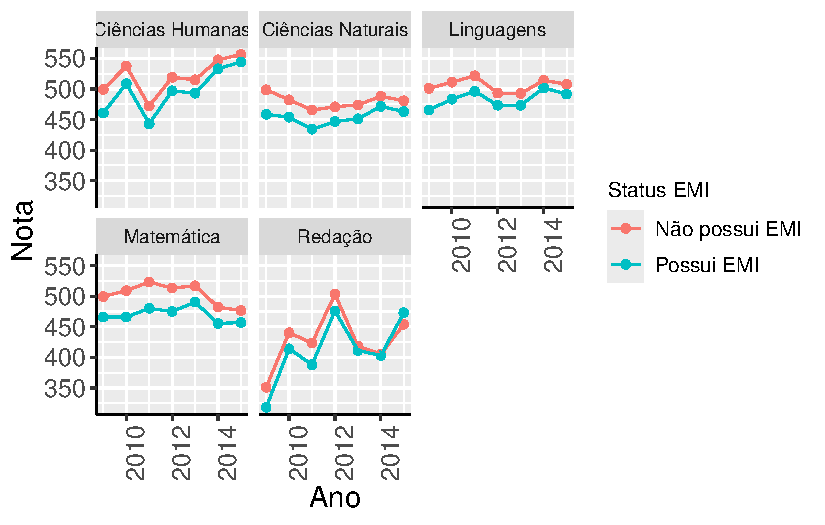
\includegraphics{script_files/figure-latex/unnamed-chunk-5-1.pdf}

\begin{Shaded}
\begin{Highlighting}[]
\NormalTok{dados\_ice\_v3 }\SpecialCharTok{\%\textgreater{}\%} 
    \FunctionTok{mutate}\NormalTok{(}\AttributeTok{ano\_enem =}\NormalTok{ lubridate}\SpecialCharTok{::}\FunctionTok{ymd}\NormalTok{(ano\_enem, }\AttributeTok{truncated =} \DecValTok{2}\NormalTok{L),}
           \AttributeTok{tratado =} \FunctionTok{as\_factor}\NormalTok{(tratado),}
           \AttributeTok{tratado =} \FunctionTok{case\_when}\NormalTok{(tratado }\SpecialCharTok{==} \DecValTok{1} \SpecialCharTok{\textasciitilde{}} \StringTok{"Possui EMI"}\NormalTok{,}
\NormalTok{                               tratado }\SpecialCharTok{!=} \DecValTok{1} \SpecialCharTok{\textasciitilde{}} \StringTok{"Não possui EMI"}\NormalTok{,}
\NormalTok{                               T }\SpecialCharTok{\textasciitilde{}}\NormalTok{ tratado)) }\SpecialCharTok{\%\textgreater{}\%}
    \FunctionTok{group\_by}\NormalTok{(ano\_enem, tratado) }\SpecialCharTok{\%\textgreater{}\%} 
    \FunctionTok{summarise}\NormalTok{(}\AttributeTok{aba\_em =} \FunctionTok{mean}\NormalTok{(aba\_em, }\AttributeTok{na.rm =}\NormalTok{ T),}
              \AttributeTok{apr\_em =} \FunctionTok{mean}\NormalTok{(apr\_em, }\AttributeTok{na.rm =}\NormalTok{ T),}
              \AttributeTok{rep\_em =} \FunctionTok{mean}\NormalTok{(rep\_em, }\AttributeTok{na.rm =}\NormalTok{ T),}
              \AttributeTok{dist\_em =} \FunctionTok{mean}\NormalTok{(dist\_em, }\AttributeTok{na.rm =}\NormalTok{ T),}
\NormalTok{              ) }\SpecialCharTok{\%\textgreater{}\%}
  \FunctionTok{pivot\_longer}\NormalTok{(}\SpecialCharTok{!}\FunctionTok{c}\NormalTok{(ano\_enem, tratado), }
               \AttributeTok{names\_to =} \StringTok{\textquotesingle{}prova\textquotesingle{}}\NormalTok{,}
               \AttributeTok{values\_to =} \StringTok{\textquotesingle{}nota\textquotesingle{}}\NormalTok{) }\SpecialCharTok{\%\textgreater{}\%} 
  \FunctionTok{mutate}\NormalTok{(}\AttributeTok{prova =} \FunctionTok{case\_when}\NormalTok{(prova }\SpecialCharTok{==} \StringTok{\textquotesingle{}aba\_em\textquotesingle{}} \SpecialCharTok{\textasciitilde{}} \StringTok{\textquotesingle{}Abandono\textquotesingle{}}\NormalTok{,}
\NormalTok{                           prova }\SpecialCharTok{==} \StringTok{\textquotesingle{}apr\_em\textquotesingle{}} \SpecialCharTok{\textasciitilde{}} \StringTok{\textquotesingle{}Aprovação\textquotesingle{}}\NormalTok{,}
\NormalTok{                           prova }\SpecialCharTok{==} \StringTok{\textquotesingle{}rep\_em\textquotesingle{}} \SpecialCharTok{\textasciitilde{}} \StringTok{\textquotesingle{}Reprovação\textquotesingle{}}\NormalTok{,}
\NormalTok{                           prova }\SpecialCharTok{==} \StringTok{\textquotesingle{}dist\_em\textquotesingle{}} \SpecialCharTok{\textasciitilde{}} \StringTok{\textquotesingle{}Distorção\textquotesingle{}}\NormalTok{,}
\NormalTok{                           T }\SpecialCharTok{\textasciitilde{}}\NormalTok{ prova)) }\SpecialCharTok{\%\textgreater{}\%} 
  \FunctionTok{ggplot}\NormalTok{() }\SpecialCharTok{+}
  \FunctionTok{geom\_point}\NormalTok{(}\FunctionTok{aes}\NormalTok{(ano\_enem, nota, }\AttributeTok{colour =}\NormalTok{ tratado)) }\SpecialCharTok{+}
  \FunctionTok{geom\_line}\NormalTok{(}\FunctionTok{aes}\NormalTok{(ano\_enem, nota, }\AttributeTok{colour =}\NormalTok{ tratado)) }\SpecialCharTok{+}
  \FunctionTok{labs}\NormalTok{(}\AttributeTok{x =} \StringTok{\textquotesingle{}Ano\textquotesingle{}}\NormalTok{, }\AttributeTok{y =} \StringTok{\textquotesingle{}Nota\textquotesingle{}}\NormalTok{, }\AttributeTok{colour =} \StringTok{"Status EMI"}\NormalTok{) }\SpecialCharTok{+}
  \FunctionTok{facet\_wrap}\NormalTok{(}\FunctionTok{vars}\NormalTok{(prova)) }\SpecialCharTok{+}
\NormalTok{  tema}
\end{Highlighting}
\end{Shaded}

\begin{verbatim}
`summarise()` has grouped output by 'ano_enem'. You can override using the
`.groups` argument.
\end{verbatim}

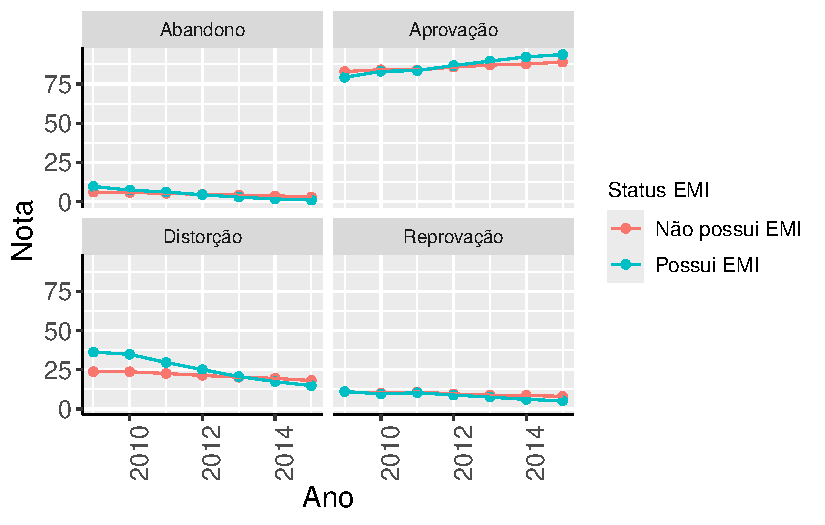
\includegraphics{script_files/figure-latex/unnamed-chunk-6-1.pdf}

\begin{Shaded}
\begin{Highlighting}[]
\NormalTok{serie\_media\_notas }\OtherTok{\textless{}{-}}
\NormalTok{  dados\_ice\_v3 }\SpecialCharTok{\%\textgreater{}\%} 
    \FunctionTok{filter}\NormalTok{(ano\_enem }\SpecialCharTok{\textgreater{}=} \DecValTok{2009}\NormalTok{) }\SpecialCharTok{\%\textgreater{}\%} 
    \FunctionTok{group\_by}\NormalTok{(ano\_enem) }\SpecialCharTok{\%\textgreater{}\%} 
     \FunctionTok{summarise}\NormalTok{(}\AttributeTok{enem\_nota\_objetiva =} \FunctionTok{mean}\NormalTok{(enem\_nota\_objetivab, }\AttributeTok{na.rm =}\NormalTok{ T),}
              \AttributeTok{enem\_nota\_redacao =} \FunctionTok{mean}\NormalTok{(enem\_nota\_redacao, }\AttributeTok{na.rm =}\NormalTok{ T),}
              \AttributeTok{enem\_nota\_matematica =} \FunctionTok{mean}\NormalTok{(enem\_nota\_matematica, }\AttributeTok{na.rm =}\NormalTok{ T),}
              \AttributeTok{enem\_nota\_linguagens =} \FunctionTok{mean}\NormalTok{(enem\_nota\_linguagens, }\AttributeTok{na.rm =}\NormalTok{ T),}
              \AttributeTok{enem\_nota\_ciencias =} \FunctionTok{mean}\NormalTok{(enem\_nota\_ciencias, }\AttributeTok{na.rm =}\NormalTok{ T),}
              \AttributeTok{enem\_nota\_humanas =} \FunctionTok{mean}\NormalTok{(enem\_nota\_humanas, }\AttributeTok{na.rm =}\NormalTok{ T)}
\NormalTok{              ) }\SpecialCharTok{\%\textgreater{}\%}
  \FunctionTok{pivot\_longer}\NormalTok{(}\SpecialCharTok{!}\NormalTok{ano\_enem, }
               \AttributeTok{names\_to =} \StringTok{\textquotesingle{}prova\textquotesingle{}}\NormalTok{,}
               \AttributeTok{values\_to =} \StringTok{\textquotesingle{}nota\textquotesingle{}}\NormalTok{) }\SpecialCharTok{\%\textgreater{}\%} 
  \FunctionTok{mutate}\NormalTok{(}\AttributeTok{prova =} \FunctionTok{case\_when}\NormalTok{(prova }\SpecialCharTok{==} \StringTok{\textquotesingle{}enem\_nota\_objetiva\textquotesingle{}} \SpecialCharTok{\textasciitilde{}} \StringTok{\textquotesingle{}Objetiva\textquotesingle{}}\NormalTok{,}
\NormalTok{                           prova }\SpecialCharTok{==} \StringTok{\textquotesingle{}enem\_nota\_redacao\textquotesingle{}} \SpecialCharTok{\textasciitilde{}} \StringTok{\textquotesingle{}Redação\textquotesingle{}}\NormalTok{,}
\NormalTok{                           prova }\SpecialCharTok{==} \StringTok{\textquotesingle{}enem\_nota\_matematica\textquotesingle{}} \SpecialCharTok{\textasciitilde{}} \StringTok{\textquotesingle{}Matemática\textquotesingle{}}\NormalTok{,}
\NormalTok{                           prova }\SpecialCharTok{==} \StringTok{\textquotesingle{}enem\_nota\_linguagens\textquotesingle{}} \SpecialCharTok{\textasciitilde{}} \StringTok{\textquotesingle{}Linguagens\textquotesingle{}}\NormalTok{,}
\NormalTok{                           prova }\SpecialCharTok{==} \StringTok{\textquotesingle{}enem\_nota\_humanas\textquotesingle{}} \SpecialCharTok{\textasciitilde{}} \StringTok{\textquotesingle{}Ciências Humanas\textquotesingle{}}\NormalTok{,}
\NormalTok{                           prova }\SpecialCharTok{==} \StringTok{\textquotesingle{}enem\_nota\_ciencias\textquotesingle{}} \SpecialCharTok{\textasciitilde{}} \StringTok{\textquotesingle{}Ciências Naturais\textquotesingle{}}\NormalTok{,}
\NormalTok{                           T }\SpecialCharTok{\textasciitilde{}}\NormalTok{ prova)) }\SpecialCharTok{\%\textgreater{}\%} 
  \FunctionTok{ggplot}\NormalTok{(}\FunctionTok{aes}\NormalTok{(ano\_enem, nota)) }\SpecialCharTok{+}
  \FunctionTok{geom\_point}\NormalTok{() }\SpecialCharTok{+}
  \FunctionTok{geom\_line}\NormalTok{() }\SpecialCharTok{+} 
  \FunctionTok{labs}\NormalTok{(}\AttributeTok{x =} \StringTok{\textquotesingle{}Ano\textquotesingle{}}\NormalTok{, }\AttributeTok{y =} \StringTok{\textquotesingle{}Nota\textquotesingle{}}\NormalTok{) }\SpecialCharTok{+}
  \FunctionTok{facet\_wrap}\NormalTok{(}\FunctionTok{vars}\NormalTok{(prova), }\AttributeTok{scales =} \StringTok{"free"}\NormalTok{) }\SpecialCharTok{+}
\NormalTok{  tema}

\FunctionTok{ggsave}\NormalTok{(serie\_media\_notas, }
       \AttributeTok{filename =} \StringTok{"G:/Meu Drive/Insper/TCC/Plots/serie\_media\_notas.pdf"}\NormalTok{,}
       \AttributeTok{device =} \StringTok{"pdf"}\NormalTok{,}
       \AttributeTok{width=}\DecValTok{12}\NormalTok{,}\AttributeTok{height=}\DecValTok{6}\NormalTok{, }\AttributeTok{units =} \StringTok{"in"}\NormalTok{)}

\NormalTok{serie\_media\_indicadores }\OtherTok{\textless{}{-}} 
\NormalTok{  painel\_indicadores\_simplificado }\SpecialCharTok{\%\textgreater{}\%} 
    \FunctionTok{mutate}\NormalTok{(}\AttributeTok{ano\_censo =}\NormalTok{ ano) }\SpecialCharTok{\%\textgreater{}\%} 
    \FunctionTok{group\_by}\NormalTok{(ano\_censo) }\SpecialCharTok{\%\textgreater{}\%} 
     \FunctionTok{summarise}\NormalTok{(}\AttributeTok{aprovacao =} \FunctionTok{mean}\NormalTok{(apr\_em, }\AttributeTok{na.rm =}\NormalTok{ T),}
              \AttributeTok{reprovacao =} \FunctionTok{mean}\NormalTok{(rep\_em, }\AttributeTok{na.rm =}\NormalTok{ T),}
              \AttributeTok{abandono =} \FunctionTok{mean}\NormalTok{(aba\_em, }\AttributeTok{na.rm =}\NormalTok{ T),}
              \AttributeTok{distorcao =} \FunctionTok{mean}\NormalTok{(dist\_em, }\AttributeTok{na.rm =}\NormalTok{ T),}
\NormalTok{              ) }\SpecialCharTok{\%\textgreater{}\%}
  \FunctionTok{pivot\_longer}\NormalTok{(}\SpecialCharTok{!}\NormalTok{ano\_censo, }
               \AttributeTok{names\_to =} \StringTok{\textquotesingle{}prova\textquotesingle{}}\NormalTok{,}
               \AttributeTok{values\_to =} \StringTok{\textquotesingle{}nota\textquotesingle{}}\NormalTok{) }\SpecialCharTok{\%\textgreater{}\%} 
  \FunctionTok{mutate}\NormalTok{(}\AttributeTok{prova =} \FunctionTok{case\_when}\NormalTok{(prova }\SpecialCharTok{==} \StringTok{\textquotesingle{}aprovacao\textquotesingle{}} \SpecialCharTok{\textasciitilde{}} \StringTok{\textquotesingle{}Aprovação\textquotesingle{}}\NormalTok{,}
\NormalTok{                           prova }\SpecialCharTok{==} \StringTok{\textquotesingle{}reprovacao\textquotesingle{}} \SpecialCharTok{\textasciitilde{}} \StringTok{\textquotesingle{}Reprovação\textquotesingle{}}\NormalTok{,}
\NormalTok{                           prova }\SpecialCharTok{==} \StringTok{\textquotesingle{}abandono\textquotesingle{}} \SpecialCharTok{\textasciitilde{}} \StringTok{\textquotesingle{}Abandono\textquotesingle{}}\NormalTok{,}
\NormalTok{                           prova }\SpecialCharTok{==} \StringTok{\textquotesingle{}distorcao\textquotesingle{}} \SpecialCharTok{\textasciitilde{}} \StringTok{\textquotesingle{}Distorção\textquotesingle{}}\NormalTok{,}
\NormalTok{                           T }\SpecialCharTok{\textasciitilde{}}\NormalTok{ prova)) }\SpecialCharTok{\%\textgreater{}\%} 
  \FunctionTok{ggplot}\NormalTok{(}\FunctionTok{aes}\NormalTok{(ano\_censo, nota)) }\SpecialCharTok{+}
  \FunctionTok{geom\_point}\NormalTok{() }\SpecialCharTok{+}
  \FunctionTok{geom\_line}\NormalTok{() }\SpecialCharTok{+} 
  \FunctionTok{labs}\NormalTok{(}\AttributeTok{x =} \StringTok{\textquotesingle{}Ano\textquotesingle{}}\NormalTok{, }\AttributeTok{y =} \StringTok{\textquotesingle{}Taxa (\%)\textquotesingle{}}\NormalTok{) }\SpecialCharTok{+}
  \FunctionTok{facet\_wrap}\NormalTok{(}\FunctionTok{vars}\NormalTok{(prova), }\AttributeTok{scales =} \StringTok{"free"}\NormalTok{) }\SpecialCharTok{+}
\NormalTok{  tema}

\FunctionTok{ggsave}\NormalTok{(serie\_media\_indicadores, }
       \AttributeTok{filename =} \StringTok{"G:/Meu Drive/Insper/TCC/Plots/serie\_media\_indicadores.pdf"}\NormalTok{,}
       \AttributeTok{device =} \StringTok{"pdf"}\NormalTok{,}
       \AttributeTok{width=}\DecValTok{12}\NormalTok{,}\AttributeTok{height=}\DecValTok{6}\NormalTok{, }\AttributeTok{units =} \StringTok{"in"}\NormalTok{) }\SpecialCharTok{+}
\NormalTok{  tema}
\end{Highlighting}
\end{Shaded}

\begin{verbatim}
NULL
\end{verbatim}

\begin{Shaded}
\begin{Highlighting}[]
\NormalTok{serie\_media\_notas}
\end{Highlighting}
\end{Shaded}

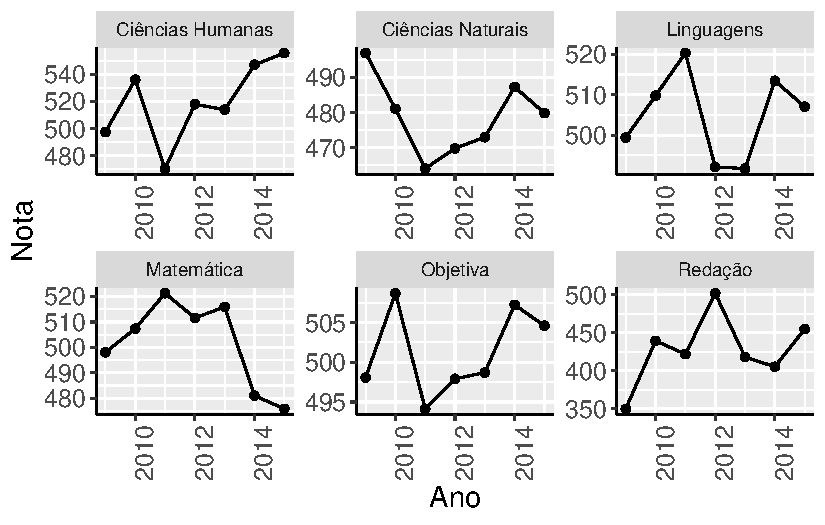
\includegraphics{script_files/figure-latex/unnamed-chunk-8-1.pdf}

\begin{Shaded}
\begin{Highlighting}[]
\NormalTok{serie\_media\_indicadores}
\end{Highlighting}
\end{Shaded}

\begin{verbatim}
Warning: Removed 3 rows containing missing values or values outside the scale range
(`geom_point()`).
\end{verbatim}

\begin{verbatim}
Warning: Removed 1 row containing missing values or values outside the scale range
(`geom_line()`).
\end{verbatim}

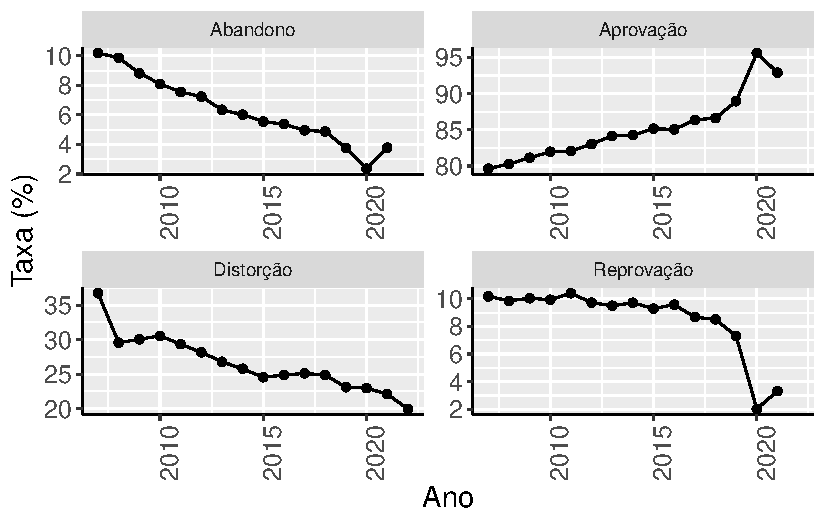
\includegraphics{script_files/figure-latex/unnamed-chunk-8-2.pdf}

\begin{Shaded}
\begin{Highlighting}[]
\NormalTok{dados\_ice\_v3 }\SpecialCharTok{\%\textgreater{}\%} 
  \FunctionTok{mutate}\NormalTok{(}\AttributeTok{tratado =} \FunctionTok{as\_factor}\NormalTok{(tratado),}
    \AttributeTok{tratado =} \FunctionTok{case\_when}\NormalTok{(tratado }\SpecialCharTok{==} \DecValTok{1} \SpecialCharTok{\textasciitilde{}} \StringTok{"Possui EMI"}\NormalTok{,}
\NormalTok{                        tratado }\SpecialCharTok{!=} \DecValTok{1} \SpecialCharTok{\textasciitilde{}} \StringTok{"Não possui EMI"}\NormalTok{,}
\NormalTok{                        T }\SpecialCharTok{\textasciitilde{}}\NormalTok{ tratado)) }\SpecialCharTok{\%\textgreater{}\%} 
  \FunctionTok{ggplot}\NormalTok{() }\SpecialCharTok{+}
  \FunctionTok{geom\_boxplot}\NormalTok{(}\FunctionTok{aes}\NormalTok{(}\AttributeTok{x =}\NormalTok{ tratado, }\AttributeTok{y =}\NormalTok{ enem\_nota\_redacao)) }\SpecialCharTok{+}
  \FunctionTok{labs}\NormalTok{(}\AttributeTok{x =}  \StringTok{\textquotesingle{}\textquotesingle{}}\NormalTok{, }\AttributeTok{y =} \StringTok{\textquotesingle{}Nota\textquotesingle{}}\NormalTok{) }\SpecialCharTok{+}
\NormalTok{  tema }\SpecialCharTok{+}
  \FunctionTok{theme}\NormalTok{(}\AttributeTok{axis.text.x =} \FunctionTok{element\_text}\NormalTok{(}\AttributeTok{angle =} \DecValTok{0}\NormalTok{, }\AttributeTok{vjust =} \FloatTok{0.5}\NormalTok{, }\AttributeTok{hjust=}\DecValTok{1}\NormalTok{))}
\end{Highlighting}
\end{Shaded}

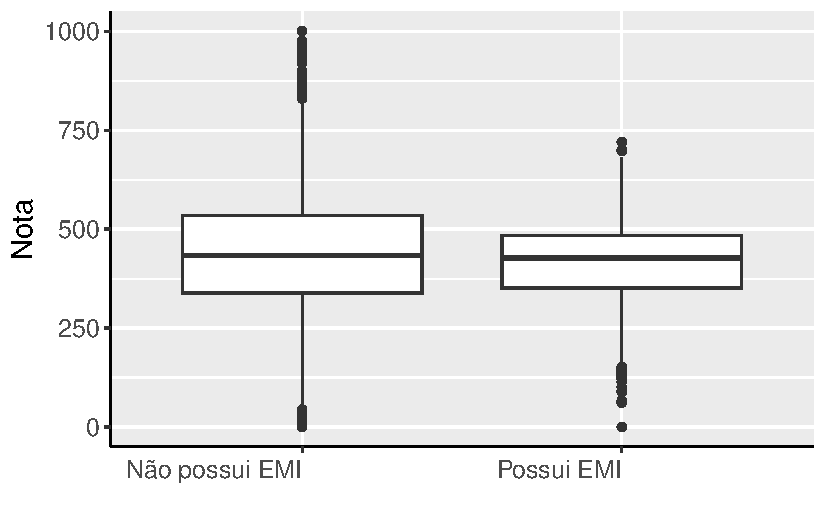
\includegraphics[width=1\textwidth,height=1\textheight]{script_files/figure-latex/unnamed-chunk-9-1.pdf}

\begin{Shaded}
\begin{Highlighting}[]
\NormalTok{dados\_ice\_v3 }\SpecialCharTok{\%\textgreater{}\%} 
  \FunctionTok{mutate}\NormalTok{(}\AttributeTok{tratado =} \FunctionTok{as\_factor}\NormalTok{(tratado),}
    \AttributeTok{tratado =} \FunctionTok{case\_when}\NormalTok{(tratado }\SpecialCharTok{==} \DecValTok{1} \SpecialCharTok{\textasciitilde{}} \StringTok{"Possui EMI"}\NormalTok{,}
\NormalTok{                        tratado }\SpecialCharTok{!=} \DecValTok{1} \SpecialCharTok{\textasciitilde{}} \StringTok{"Não possui EMI"}\NormalTok{,}
\NormalTok{                        T }\SpecialCharTok{\textasciitilde{}}\NormalTok{ tratado)) }\SpecialCharTok{\%\textgreater{}\%} 
  \FunctionTok{ggplot}\NormalTok{() }\SpecialCharTok{+}
  \FunctionTok{geom\_boxplot}\NormalTok{(}\FunctionTok{aes}\NormalTok{(}\AttributeTok{x =}\NormalTok{ tratado, }\AttributeTok{y =}\NormalTok{ enem\_nota\_matematica)) }\SpecialCharTok{+}
  \FunctionTok{labs}\NormalTok{(}\AttributeTok{x =}  \StringTok{\textquotesingle{}\textquotesingle{}}\NormalTok{, }\AttributeTok{y =} \StringTok{\textquotesingle{}Nota\textquotesingle{}}\NormalTok{) }\SpecialCharTok{+}
\NormalTok{  tema }\SpecialCharTok{+}
  \FunctionTok{theme}\NormalTok{(}\AttributeTok{axis.text.x =} \FunctionTok{element\_text}\NormalTok{(}\AttributeTok{angle =} \DecValTok{0}\NormalTok{, }\AttributeTok{vjust =} \FloatTok{0.5}\NormalTok{, }\AttributeTok{hjust=}\DecValTok{1}\NormalTok{))}
\end{Highlighting}
\end{Shaded}

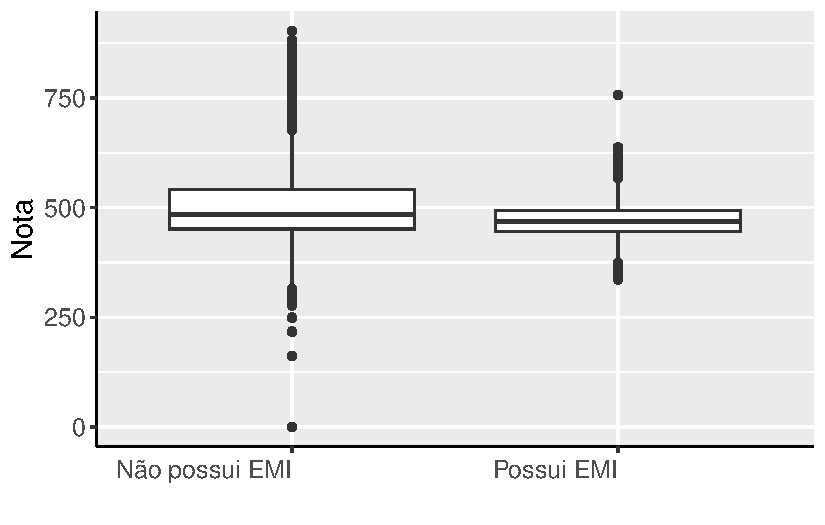
\includegraphics[width=1\textwidth,height=1\textheight]{script_files/figure-latex/unnamed-chunk-9-2.pdf}

\begin{Shaded}
\begin{Highlighting}[]
\NormalTok{dados\_ice\_v3 }\SpecialCharTok{\%\textgreater{}\%} 
  \FunctionTok{mutate}\NormalTok{(}\AttributeTok{tratado =} \FunctionTok{as\_factor}\NormalTok{(tratado),}
    \AttributeTok{tratado =} \FunctionTok{case\_when}\NormalTok{(tratado }\SpecialCharTok{==} \DecValTok{1} \SpecialCharTok{\textasciitilde{}} \StringTok{"Possui EMI"}\NormalTok{,}
\NormalTok{                        tratado }\SpecialCharTok{!=} \DecValTok{1} \SpecialCharTok{\textasciitilde{}} \StringTok{"Não possui EMI"}\NormalTok{,}
\NormalTok{                        T }\SpecialCharTok{\textasciitilde{}}\NormalTok{ tratado)) }\SpecialCharTok{\%\textgreater{}\%} 
  \FunctionTok{ggplot}\NormalTok{() }\SpecialCharTok{+}
  \FunctionTok{geom\_boxplot}\NormalTok{(}\FunctionTok{aes}\NormalTok{(}\AttributeTok{x =}\NormalTok{ tratado, }\AttributeTok{y =}\NormalTok{ enem\_nota\_linguagens)) }\SpecialCharTok{+}
  \FunctionTok{labs}\NormalTok{(}\AttributeTok{x =}  \StringTok{\textquotesingle{}\textquotesingle{}}\NormalTok{, }\AttributeTok{y =} \StringTok{\textquotesingle{}Nota\textquotesingle{}}\NormalTok{) }\SpecialCharTok{+}
\NormalTok{  tema }\SpecialCharTok{+}
  \FunctionTok{theme}\NormalTok{(}\AttributeTok{axis.text.x =} \FunctionTok{element\_text}\NormalTok{(}\AttributeTok{angle =} \DecValTok{0}\NormalTok{, }\AttributeTok{vjust =} \FloatTok{0.5}\NormalTok{, }\AttributeTok{hjust=}\DecValTok{1}\NormalTok{))}
\end{Highlighting}
\end{Shaded}

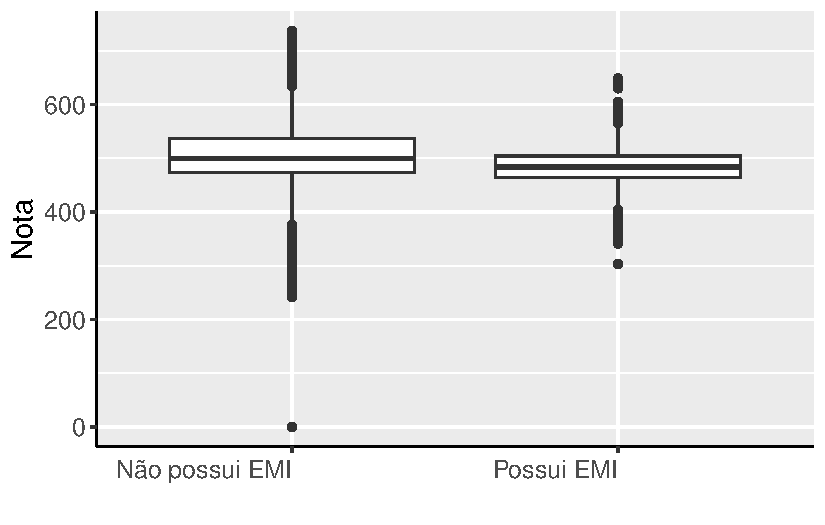
\includegraphics[width=1\textwidth,height=1\textheight]{script_files/figure-latex/unnamed-chunk-9-3.pdf}

\begin{Shaded}
\begin{Highlighting}[]
\NormalTok{dados\_ice\_v3 }\SpecialCharTok{\%\textgreater{}\%} 
  \FunctionTok{mutate}\NormalTok{(}\AttributeTok{tratado =} \FunctionTok{as\_factor}\NormalTok{(tratado),}
    \AttributeTok{tratado =} \FunctionTok{case\_when}\NormalTok{(tratado }\SpecialCharTok{==} \DecValTok{1} \SpecialCharTok{\textasciitilde{}} \StringTok{"Possui EMI"}\NormalTok{,}
\NormalTok{                        tratado }\SpecialCharTok{!=} \DecValTok{1} \SpecialCharTok{\textasciitilde{}} \StringTok{"Não possui EMI"}\NormalTok{,}
\NormalTok{                        T }\SpecialCharTok{\textasciitilde{}}\NormalTok{ tratado)) }\SpecialCharTok{\%\textgreater{}\%} 
  \FunctionTok{ggplot}\NormalTok{() }\SpecialCharTok{+}
  \FunctionTok{geom\_boxplot}\NormalTok{(}\FunctionTok{aes}\NormalTok{(}\AttributeTok{x =}\NormalTok{ tratado, }\AttributeTok{y =}\NormalTok{ enem\_nota\_humanas)) }\SpecialCharTok{+}
  \FunctionTok{labs}\NormalTok{(}\AttributeTok{x =}  \StringTok{\textquotesingle{}\textquotesingle{}}\NormalTok{, }\AttributeTok{y =} \StringTok{\textquotesingle{}Nota\textquotesingle{}}\NormalTok{) }\SpecialCharTok{+}
\NormalTok{  tema }\SpecialCharTok{+}
  \FunctionTok{theme}\NormalTok{(}\AttributeTok{axis.text.x =} \FunctionTok{element\_text}\NormalTok{(}\AttributeTok{angle =} \DecValTok{0}\NormalTok{, }\AttributeTok{vjust =} \FloatTok{0.5}\NormalTok{, }\AttributeTok{hjust=}\DecValTok{1}\NormalTok{))}
\end{Highlighting}
\end{Shaded}

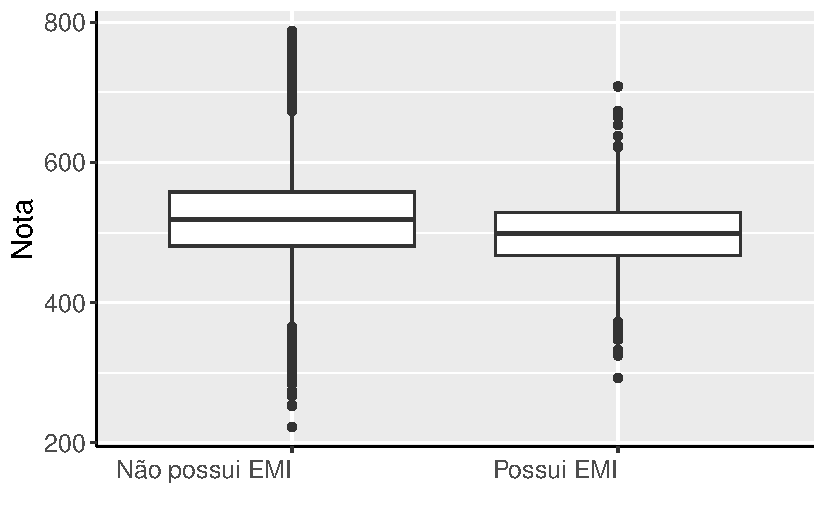
\includegraphics[width=1\textwidth,height=1\textheight]{script_files/figure-latex/unnamed-chunk-9-4.pdf}

\begin{Shaded}
\begin{Highlighting}[]
\NormalTok{dados\_ice\_v3 }\SpecialCharTok{\%\textgreater{}\%} 
  \FunctionTok{mutate}\NormalTok{(}\AttributeTok{tratado =} \FunctionTok{as\_factor}\NormalTok{(tratado),}
    \AttributeTok{tratado =} \FunctionTok{case\_when}\NormalTok{(tratado }\SpecialCharTok{==} \DecValTok{1} \SpecialCharTok{\textasciitilde{}} \StringTok{"Possui EMI"}\NormalTok{,}
\NormalTok{                        tratado }\SpecialCharTok{!=} \DecValTok{1} \SpecialCharTok{\textasciitilde{}} \StringTok{"Não possui EMI"}\NormalTok{,}
\NormalTok{                        T }\SpecialCharTok{\textasciitilde{}}\NormalTok{ tratado)) }\SpecialCharTok{\%\textgreater{}\%} 
  \FunctionTok{ggplot}\NormalTok{() }\SpecialCharTok{+}
  \FunctionTok{geom\_boxplot}\NormalTok{(}\FunctionTok{aes}\NormalTok{(}\AttributeTok{x =}\NormalTok{ tratado, }\AttributeTok{y =}\NormalTok{ enem\_nota\_ciencias)) }\SpecialCharTok{+}
  \FunctionTok{labs}\NormalTok{(}\AttributeTok{x =}  \StringTok{\textquotesingle{}\textquotesingle{}}\NormalTok{, }\AttributeTok{y =} \StringTok{\textquotesingle{}Nota\textquotesingle{}}\NormalTok{) }\SpecialCharTok{+}
\NormalTok{  tema }\SpecialCharTok{+}
  \FunctionTok{theme}\NormalTok{(}\AttributeTok{axis.text.x =} \FunctionTok{element\_text}\NormalTok{(}\AttributeTok{angle =} \DecValTok{0}\NormalTok{, }\AttributeTok{vjust =} \FloatTok{0.5}\NormalTok{, }\AttributeTok{hjust=}\DecValTok{1}\NormalTok{))}
\end{Highlighting}
\end{Shaded}

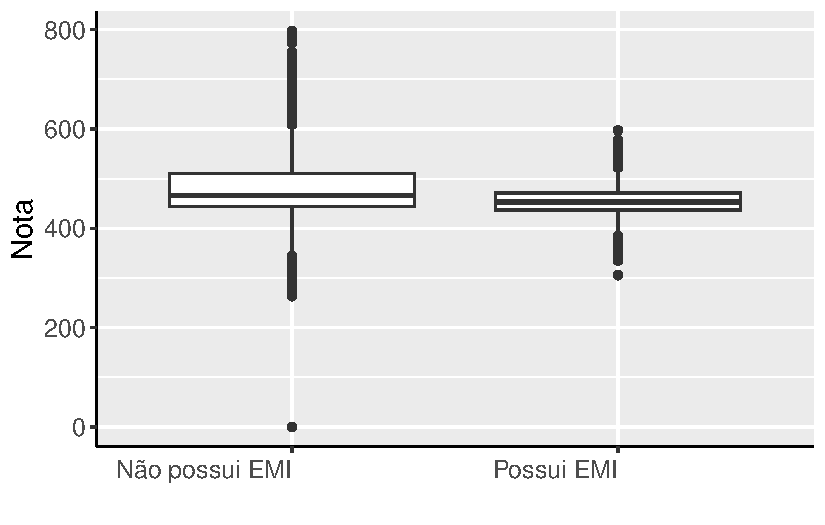
\includegraphics[width=1\textwidth,height=1\textheight]{script_files/figure-latex/unnamed-chunk-9-5.pdf}

\begin{Shaded}
\begin{Highlighting}[]
\NormalTok{dados\_ice\_v3 }\SpecialCharTok{\%\textgreater{}\%} 
  \FunctionTok{filter}\NormalTok{(ano\_enem }\SpecialCharTok{\textgreater{}=} \DecValTok{2009}\NormalTok{) }\SpecialCharTok{\%\textgreater{}\%} 
    \FunctionTok{mutate}\NormalTok{(}\AttributeTok{ano\_enem =} \FunctionTok{as.factor}\NormalTok{(ano\_enem),}
           \AttributeTok{tratado =} \FunctionTok{as\_factor}\NormalTok{(tratado),}
           \AttributeTok{tratado =} \FunctionTok{case\_when}\NormalTok{(tratado }\SpecialCharTok{==} \DecValTok{1} \SpecialCharTok{\textasciitilde{}} \StringTok{"Possui EMI"}\NormalTok{,}
\NormalTok{                               tratado }\SpecialCharTok{!=} \DecValTok{1} \SpecialCharTok{\textasciitilde{}} \StringTok{"Não possui EMI"}\NormalTok{,}
\NormalTok{                               T }\SpecialCharTok{\textasciitilde{}}\NormalTok{ tratado)) }\SpecialCharTok{\%\textgreater{}\%}
    \FunctionTok{group\_by}\NormalTok{(ano\_enem, tratado) }\SpecialCharTok{\%\textgreater{}\%} 
    \FunctionTok{summarise}\NormalTok{(}\AttributeTok{enem\_nota\_redacao =} \FunctionTok{mean}\NormalTok{(enem\_nota\_redacao, }\AttributeTok{na.rm =}\NormalTok{ T),}
              \AttributeTok{enem\_nota\_matematica =} \FunctionTok{mean}\NormalTok{(enem\_nota\_matematica, }\AttributeTok{na.rm =}\NormalTok{ T),}
              \AttributeTok{enem\_nota\_linguagens =} \FunctionTok{mean}\NormalTok{(enem\_nota\_linguagens, }\AttributeTok{na.rm =}\NormalTok{ T),}
              \AttributeTok{enem\_nota\_ciencias =} \FunctionTok{mean}\NormalTok{(enem\_nota\_ciencias, }\AttributeTok{na.rm =}\NormalTok{ T),}
              \AttributeTok{enem\_nota\_humanas =} \FunctionTok{mean}\NormalTok{(enem\_nota\_humanas, }\AttributeTok{na.rm =}\NormalTok{ T)}
\NormalTok{              ) }\SpecialCharTok{\%\textgreater{}\%}
  \FunctionTok{pivot\_longer}\NormalTok{(}\SpecialCharTok{!}\FunctionTok{c}\NormalTok{(ano\_enem, tratado), }
               \AttributeTok{names\_to =} \StringTok{\textquotesingle{}prova\textquotesingle{}}\NormalTok{,}
               \AttributeTok{values\_to =} \StringTok{\textquotesingle{}nota\textquotesingle{}}\NormalTok{) }\SpecialCharTok{\%\textgreater{}\%} 
  \FunctionTok{mutate}\NormalTok{(}\AttributeTok{prova =} \FunctionTok{case\_when}\NormalTok{(prova }\SpecialCharTok{==} \StringTok{\textquotesingle{}enem\_nota\_objetiva\textquotesingle{}} \SpecialCharTok{\textasciitilde{}} \StringTok{\textquotesingle{}Objetiva\textquotesingle{}}\NormalTok{,}
\NormalTok{                           prova }\SpecialCharTok{==} \StringTok{\textquotesingle{}enem\_nota\_redacao\textquotesingle{}} \SpecialCharTok{\textasciitilde{}} \StringTok{\textquotesingle{}Redação\textquotesingle{}}\NormalTok{,}
\NormalTok{                           prova }\SpecialCharTok{==} \StringTok{\textquotesingle{}enem\_nota\_matematica\textquotesingle{}} \SpecialCharTok{\textasciitilde{}} \StringTok{\textquotesingle{}Matemática\textquotesingle{}}\NormalTok{,}
\NormalTok{                           prova }\SpecialCharTok{==} \StringTok{\textquotesingle{}enem\_nota\_linguagens\textquotesingle{}} \SpecialCharTok{\textasciitilde{}} \StringTok{\textquotesingle{}Linguagens\textquotesingle{}}\NormalTok{,}
\NormalTok{                           prova }\SpecialCharTok{==} \StringTok{\textquotesingle{}enem\_nota\_humanas\textquotesingle{}} \SpecialCharTok{\textasciitilde{}} \StringTok{\textquotesingle{}Ciências Humanas\textquotesingle{}}\NormalTok{,}
\NormalTok{                           prova }\SpecialCharTok{==} \StringTok{\textquotesingle{}enem\_nota\_ciencias\textquotesingle{}} \SpecialCharTok{\textasciitilde{}} \StringTok{\textquotesingle{}Ciências Naturais\textquotesingle{}}\NormalTok{,}
\NormalTok{                           T }\SpecialCharTok{\textasciitilde{}}\NormalTok{ prova)) }\SpecialCharTok{\%\textgreater{}\%} 
  \FunctionTok{filter}\NormalTok{(prova }\SpecialCharTok{!=} \StringTok{\textquotesingle{}Redação\textquotesingle{}}\NormalTok{) }\SpecialCharTok{\%\textgreater{}\%} 
  \FunctionTok{ggplot}\NormalTok{() }\SpecialCharTok{+}
  \FunctionTok{geom\_point}\NormalTok{(}\FunctionTok{aes}\NormalTok{(ano\_enem, nota, }\AttributeTok{colour =}\NormalTok{ tratado)) }\SpecialCharTok{+}
  \FunctionTok{labs}\NormalTok{(}\AttributeTok{x =} \StringTok{\textquotesingle{}Ano\textquotesingle{}}\NormalTok{, }\AttributeTok{y =} \StringTok{\textquotesingle{}Nota\textquotesingle{}}\NormalTok{, }\AttributeTok{colour =} \StringTok{"Status EMI"}\NormalTok{) }\SpecialCharTok{+}
  \FunctionTok{facet\_wrap}\NormalTok{(}\FunctionTok{vars}\NormalTok{(prova), }\AttributeTok{scales =} \StringTok{"free"}\NormalTok{)}
\end{Highlighting}
\end{Shaded}

\begin{verbatim}
`summarise()` has grouped output by 'ano_enem'. You can override using the
`.groups` argument.
\end{verbatim}

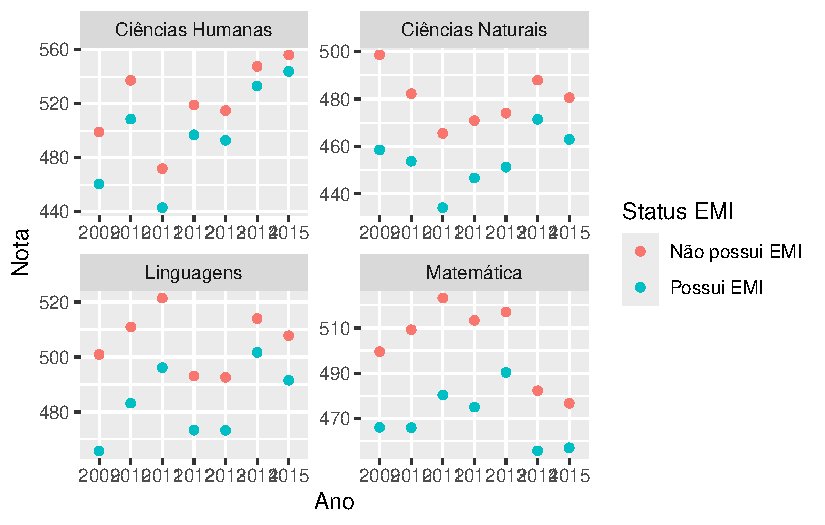
\includegraphics[width=1\textwidth,height=1\textheight]{script_files/figure-latex/unnamed-chunk-10-1.pdf}

\begin{Shaded}
\begin{Highlighting}[]
\NormalTok{painel\_indicadores\_simplificado }\SpecialCharTok{\%\textgreater{}\%} 
  \FunctionTok{mutate}\NormalTok{(}\AttributeTok{ano\_censo =} \FunctionTok{as.factor}\NormalTok{(ano\_censo.x),}
         \AttributeTok{tratado =} \FunctionTok{as\_factor}\NormalTok{(tratado),}
         \AttributeTok{tratado =} \FunctionTok{case\_when}\NormalTok{(tratado }\SpecialCharTok{==} \DecValTok{1} \SpecialCharTok{\textasciitilde{}} \StringTok{"Possui EMI"}\NormalTok{,}
\NormalTok{                             tratado }\SpecialCharTok{!=} \DecValTok{1} \SpecialCharTok{\textasciitilde{}} \StringTok{"Não possui EMI"}\NormalTok{,}
\NormalTok{                             T }\SpecialCharTok{\textasciitilde{}}\NormalTok{ tratado),}
         \AttributeTok{tratado =} \FunctionTok{as\_factor}\NormalTok{(tratado)) }\SpecialCharTok{\%\textgreater{}\%} 
  \FunctionTok{group\_by}\NormalTok{(ano\_censo,tratado) }\SpecialCharTok{\%\textgreater{}\%} 
  \FunctionTok{summarise}\NormalTok{(}\AttributeTok{aprovacao =} \FunctionTok{mean}\NormalTok{(apr\_em, }\AttributeTok{na.rm =}\NormalTok{ T),}
            \AttributeTok{reprovacao =} \FunctionTok{mean}\NormalTok{(rep\_em, }\AttributeTok{na.rm =}\NormalTok{ T),}
            \AttributeTok{abandono =} \FunctionTok{mean}\NormalTok{(aba\_em, }\AttributeTok{na.rm =}\NormalTok{ T),}
            \AttributeTok{distorcao =} \FunctionTok{mean}\NormalTok{(dist\_em, }\AttributeTok{na.rm =}\NormalTok{ T),}
\NormalTok{            ) }\SpecialCharTok{\%\textgreater{}\%}
\FunctionTok{pivot\_longer}\NormalTok{(}\SpecialCharTok{!}\FunctionTok{c}\NormalTok{(ano\_censo,tratado), }
             \AttributeTok{names\_to =} \StringTok{\textquotesingle{}prova\textquotesingle{}}\NormalTok{,}
             \AttributeTok{values\_to =} \StringTok{\textquotesingle{}nota\textquotesingle{}}\NormalTok{) }\SpecialCharTok{\%\textgreater{}\%} 
\FunctionTok{mutate}\NormalTok{(}\AttributeTok{prova =} \FunctionTok{case\_when}\NormalTok{(prova }\SpecialCharTok{==} \StringTok{\textquotesingle{}aprovacao\textquotesingle{}} \SpecialCharTok{\textasciitilde{}} \StringTok{\textquotesingle{}Aprovação\textquotesingle{}}\NormalTok{,}
\NormalTok{                         prova }\SpecialCharTok{==} \StringTok{\textquotesingle{}reprovacao\textquotesingle{}} \SpecialCharTok{\textasciitilde{}} \StringTok{\textquotesingle{}Reprovação\textquotesingle{}}\NormalTok{,}
\NormalTok{                         prova }\SpecialCharTok{==} \StringTok{\textquotesingle{}abandono\textquotesingle{}} \SpecialCharTok{\textasciitilde{}} \StringTok{\textquotesingle{}Abandono\textquotesingle{}}\NormalTok{,}
\NormalTok{                         prova }\SpecialCharTok{==} \StringTok{\textquotesingle{}distorcao\textquotesingle{}} \SpecialCharTok{\textasciitilde{}} \StringTok{\textquotesingle{}Distorção\textquotesingle{}}\NormalTok{,}
\NormalTok{                         T }\SpecialCharTok{\textasciitilde{}}\NormalTok{ prova)) }\SpecialCharTok{\%\textgreater{}\%} 
  \FunctionTok{ggplot}\NormalTok{() }\SpecialCharTok{+}
  \FunctionTok{geom\_point}\NormalTok{(}\FunctionTok{aes}\NormalTok{(ano\_censo, nota, }\AttributeTok{colour =}\NormalTok{ tratado)) }\SpecialCharTok{+}
  \FunctionTok{labs}\NormalTok{(}\AttributeTok{x =} \StringTok{\textquotesingle{}Ano\textquotesingle{}}\NormalTok{, }\AttributeTok{y =} \StringTok{\textquotesingle{}Taxa (\%)\textquotesingle{}}\NormalTok{) }\SpecialCharTok{+}
  \FunctionTok{facet\_wrap}\NormalTok{(}\FunctionTok{vars}\NormalTok{(prova), }\AttributeTok{scales =} \StringTok{"free"}\NormalTok{)}
\end{Highlighting}
\end{Shaded}

\begin{verbatim}
`summarise()` has grouped output by 'ano_censo'. You can override using the
`.groups` argument.
\end{verbatim}

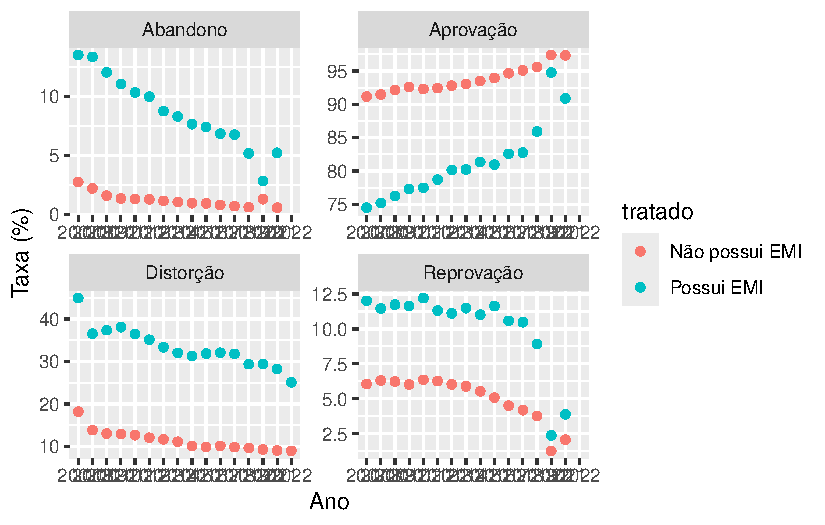
\includegraphics[width=1\textwidth,height=1\textheight]{script_files/figure-latex/unnamed-chunk-10-2.pdf}

\begin{Shaded}
\begin{Highlighting}[]
\NormalTok{dados\_ice\_v3 }\SpecialCharTok{\%\textgreater{}\%}
  \FunctionTok{filter}\NormalTok{(ano\_enem }\SpecialCharTok{\textgreater{}=} \DecValTok{2009}\NormalTok{, tratado }\SpecialCharTok{==} \DecValTok{1}\NormalTok{) }\SpecialCharTok{\%\textgreater{}\%}
  \FunctionTok{mutate}\NormalTok{(}\AttributeTok{ano\_enem =} \FunctionTok{as.factor}\NormalTok{(ano\_enem), }\AttributeTok{ano\_ice =} \FunctionTok{as.factor}\NormalTok{(ano\_ice)) }\SpecialCharTok{\%\textgreater{}\%}
  \FunctionTok{group\_by}\NormalTok{(ano\_enem, ano\_ice) }\SpecialCharTok{\%\textgreater{}\%}
  \FunctionTok{summarise}\NormalTok{(}
    \AttributeTok{enem\_nota\_redacao =} \FunctionTok{mean}\NormalTok{(enem\_nota\_redacao, }\AttributeTok{na.rm =} \ConstantTok{TRUE}\NormalTok{),}
    \AttributeTok{enem\_nota\_matematica =} \FunctionTok{mean}\NormalTok{(enem\_nota\_matematica, }\AttributeTok{na.rm =} \ConstantTok{TRUE}\NormalTok{),}
    \AttributeTok{enem\_nota\_linguagens =} \FunctionTok{mean}\NormalTok{(enem\_nota\_linguagens, }\AttributeTok{na.rm =} \ConstantTok{TRUE}\NormalTok{),}
    \AttributeTok{enem\_nota\_ciencias =} \FunctionTok{mean}\NormalTok{(enem\_nota\_ciencias, }\AttributeTok{na.rm =} \ConstantTok{TRUE}\NormalTok{),}
    \AttributeTok{enem\_nota\_humanas =} \FunctionTok{mean}\NormalTok{(enem\_nota\_humanas, }\AttributeTok{na.rm =} \ConstantTok{TRUE}\NormalTok{),}
    \AttributeTok{enem\_nota\_objetiva =} \FunctionTok{mean}\NormalTok{(enem\_nota\_objetivab, }\AttributeTok{na.rm =} \ConstantTok{TRUE}\NormalTok{),}
    \AttributeTok{.groups =} \StringTok{"drop"}  \CommentTok{\# Override grouping}
\NormalTok{  ) }\SpecialCharTok{\%\textgreater{}\%}
  \FunctionTok{ungroup}\NormalTok{() }\SpecialCharTok{\%\textgreater{}\%}
  \FunctionTok{pivot\_longer}\NormalTok{(}
    \SpecialCharTok{!}\FunctionTok{c}\NormalTok{(ano\_enem, ano\_ice),}
    \AttributeTok{names\_to =} \StringTok{\textquotesingle{}prova\textquotesingle{}}\NormalTok{,}
    \AttributeTok{values\_to =} \StringTok{\textquotesingle{}nota\textquotesingle{}}
\NormalTok{  ) }\SpecialCharTok{\%\textgreater{}\%}
  \FunctionTok{mutate}\NormalTok{(}
    \AttributeTok{prova =} \FunctionTok{case\_when}\NormalTok{(}
\NormalTok{      prova }\SpecialCharTok{==} \StringTok{\textquotesingle{}enem\_nota\_objetiva\textquotesingle{}} \SpecialCharTok{\textasciitilde{}} \StringTok{\textquotesingle{}Objetiva\textquotesingle{}}\NormalTok{,}
\NormalTok{      prova }\SpecialCharTok{==} \StringTok{\textquotesingle{}enem\_nota\_redacao\textquotesingle{}} \SpecialCharTok{\textasciitilde{}} \StringTok{\textquotesingle{}Redação\textquotesingle{}}\NormalTok{,}
\NormalTok{      prova }\SpecialCharTok{==} \StringTok{\textquotesingle{}enem\_nota\_matematica\textquotesingle{}} \SpecialCharTok{\textasciitilde{}} \StringTok{\textquotesingle{}Matemática\textquotesingle{}}\NormalTok{,}
\NormalTok{      prova }\SpecialCharTok{==} \StringTok{\textquotesingle{}enem\_nota\_linguagens\textquotesingle{}} \SpecialCharTok{\textasciitilde{}} \StringTok{\textquotesingle{}Linguagens\textquotesingle{}}\NormalTok{,}
\NormalTok{      prova }\SpecialCharTok{==} \StringTok{\textquotesingle{}enem\_nota\_humanas\textquotesingle{}} \SpecialCharTok{\textasciitilde{}} \StringTok{\textquotesingle{}Ciências Humanas\textquotesingle{}}\NormalTok{,}
\NormalTok{      prova }\SpecialCharTok{==} \StringTok{\textquotesingle{}enem\_nota\_ciencias\textquotesingle{}} \SpecialCharTok{\textasciitilde{}} \StringTok{\textquotesingle{}Ciências Naturais\textquotesingle{}}\NormalTok{,}
      \ConstantTok{TRUE} \SpecialCharTok{\textasciitilde{}}\NormalTok{ prova}
\NormalTok{    )}
\NormalTok{  ) }\SpecialCharTok{\%\textgreater{}\%}
  \FunctionTok{filter}\NormalTok{(prova }\SpecialCharTok{==} \StringTok{\textquotesingle{}Objetiva\textquotesingle{}}\NormalTok{) }\SpecialCharTok{\%\textgreater{}\%} 
  \FunctionTok{ggplot}\NormalTok{() }\SpecialCharTok{+}
  \FunctionTok{geom\_line}\NormalTok{(}\FunctionTok{aes}\NormalTok{(ano\_enem, nota, }\AttributeTok{group =}\NormalTok{ ano\_ice)) }\SpecialCharTok{+}
  \FunctionTok{labs}\NormalTok{(}\AttributeTok{x =} \StringTok{\textquotesingle{}Ano\textquotesingle{}}\NormalTok{, }\AttributeTok{y =} \StringTok{\textquotesingle{}Nota Objetiva\textquotesingle{}}\NormalTok{) }\SpecialCharTok{+}
  \FunctionTok{facet\_wrap}\NormalTok{(}\FunctionTok{vars}\NormalTok{(ano\_ice), }\AttributeTok{scales =} \StringTok{"free"}\NormalTok{)}
\end{Highlighting}
\end{Shaded}

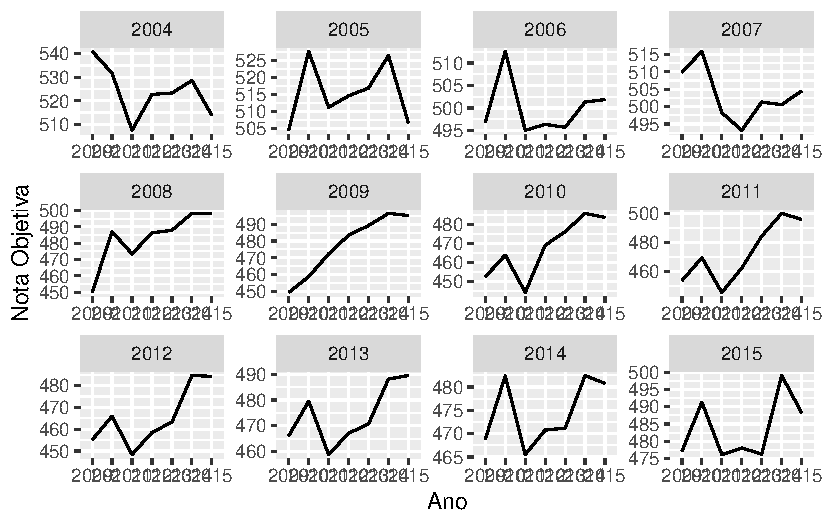
\includegraphics{script_files/figure-latex/unnamed-chunk-11-1.pdf}

\begin{Shaded}
\begin{Highlighting}[]
\NormalTok{dados\_ice\_v3 }\SpecialCharTok{\%\textgreater{}\%}
  \FunctionTok{filter}\NormalTok{(ano\_enem }\SpecialCharTok{\textgreater{}=} \DecValTok{2009}\NormalTok{, tratado }\SpecialCharTok{==} \DecValTok{1}\NormalTok{) }\SpecialCharTok{\%\textgreater{}\%}
  \FunctionTok{mutate}\NormalTok{(}\AttributeTok{ano\_enem =} \FunctionTok{as.factor}\NormalTok{(ano\_enem), }\AttributeTok{ano\_ice =} \FunctionTok{as.factor}\NormalTok{(ano\_ice)) }\SpecialCharTok{\%\textgreater{}\%}
  \FunctionTok{group\_by}\NormalTok{(ano\_enem, ano\_ice) }\SpecialCharTok{\%\textgreater{}\%}
  \FunctionTok{summarise}\NormalTok{(}
    \AttributeTok{enem\_nota\_redacao =} \FunctionTok{mean}\NormalTok{(enem\_nota\_redacao, }\AttributeTok{na.rm =} \ConstantTok{TRUE}\NormalTok{),}
    \AttributeTok{enem\_nota\_matematica =} \FunctionTok{mean}\NormalTok{(enem\_nota\_matematica, }\AttributeTok{na.rm =} \ConstantTok{TRUE}\NormalTok{),}
    \AttributeTok{enem\_nota\_linguagens =} \FunctionTok{mean}\NormalTok{(enem\_nota\_linguagens, }\AttributeTok{na.rm =} \ConstantTok{TRUE}\NormalTok{),}
    \AttributeTok{enem\_nota\_ciencias =} \FunctionTok{mean}\NormalTok{(enem\_nota\_ciencias, }\AttributeTok{na.rm =} \ConstantTok{TRUE}\NormalTok{),}
    \AttributeTok{enem\_nota\_humanas =} \FunctionTok{mean}\NormalTok{(enem\_nota\_humanas, }\AttributeTok{na.rm =} \ConstantTok{TRUE}\NormalTok{),}
    \AttributeTok{enem\_nota\_objetiva =} \FunctionTok{mean}\NormalTok{(enem\_nota\_objetivab, }\AttributeTok{na.rm =} \ConstantTok{TRUE}\NormalTok{),}
    \AttributeTok{.groups =} \StringTok{"drop"}  \CommentTok{\# Override grouping}
\NormalTok{  ) }\SpecialCharTok{\%\textgreater{}\%}
  \FunctionTok{ungroup}\NormalTok{() }\SpecialCharTok{\%\textgreater{}\%}
  \FunctionTok{pivot\_longer}\NormalTok{(}
    \SpecialCharTok{!}\FunctionTok{c}\NormalTok{(ano\_enem, ano\_ice),}
    \AttributeTok{names\_to =} \StringTok{\textquotesingle{}prova\textquotesingle{}}\NormalTok{,}
    \AttributeTok{values\_to =} \StringTok{\textquotesingle{}nota\textquotesingle{}}
\NormalTok{  ) }\SpecialCharTok{\%\textgreater{}\%}
  \FunctionTok{mutate}\NormalTok{(}
    \AttributeTok{prova =} \FunctionTok{case\_when}\NormalTok{(}
\NormalTok{      prova }\SpecialCharTok{==} \StringTok{\textquotesingle{}enem\_nota\_objetiva\textquotesingle{}} \SpecialCharTok{\textasciitilde{}} \StringTok{\textquotesingle{}Objetiva\textquotesingle{}}\NormalTok{,}
\NormalTok{      prova }\SpecialCharTok{==} \StringTok{\textquotesingle{}enem\_nota\_redacao\textquotesingle{}} \SpecialCharTok{\textasciitilde{}} \StringTok{\textquotesingle{}Redação\textquotesingle{}}\NormalTok{,}
\NormalTok{      prova }\SpecialCharTok{==} \StringTok{\textquotesingle{}enem\_nota\_matematica\textquotesingle{}} \SpecialCharTok{\textasciitilde{}} \StringTok{\textquotesingle{}Matemática\textquotesingle{}}\NormalTok{,}
\NormalTok{      prova }\SpecialCharTok{==} \StringTok{\textquotesingle{}enem\_nota\_linguagens\textquotesingle{}} \SpecialCharTok{\textasciitilde{}} \StringTok{\textquotesingle{}Linguagens\textquotesingle{}}\NormalTok{,}
\NormalTok{      prova }\SpecialCharTok{==} \StringTok{\textquotesingle{}enem\_nota\_humanas\textquotesingle{}} \SpecialCharTok{\textasciitilde{}} \StringTok{\textquotesingle{}Ciências Humanas\textquotesingle{}}\NormalTok{,}
\NormalTok{      prova }\SpecialCharTok{==} \StringTok{\textquotesingle{}enem\_nota\_ciencias\textquotesingle{}} \SpecialCharTok{\textasciitilde{}} \StringTok{\textquotesingle{}Ciências Naturais\textquotesingle{}}\NormalTok{,}
      \ConstantTok{TRUE} \SpecialCharTok{\textasciitilde{}}\NormalTok{ prova}
\NormalTok{    )}
\NormalTok{  ) }\SpecialCharTok{\%\textgreater{}\%}
  \FunctionTok{filter}\NormalTok{(prova }\SpecialCharTok{==} \StringTok{\textquotesingle{}Redação\textquotesingle{}}\NormalTok{) }\SpecialCharTok{\%\textgreater{}\%} 
  \FunctionTok{ggplot}\NormalTok{() }\SpecialCharTok{+}
  \FunctionTok{geom\_line}\NormalTok{(}\FunctionTok{aes}\NormalTok{(ano\_enem, nota, }\AttributeTok{group =}\NormalTok{ ano\_ice)) }\SpecialCharTok{+}
  \FunctionTok{labs}\NormalTok{(}\AttributeTok{x =} \StringTok{\textquotesingle{}Ano\textquotesingle{}}\NormalTok{, }\AttributeTok{y =} \StringTok{\textquotesingle{}Nota Objetiva\textquotesingle{}}\NormalTok{) }\SpecialCharTok{+}
  \FunctionTok{facet\_wrap}\NormalTok{(}\FunctionTok{vars}\NormalTok{(ano\_ice), }\AttributeTok{scales =} \StringTok{"free"}\NormalTok{)}
\end{Highlighting}
\end{Shaded}

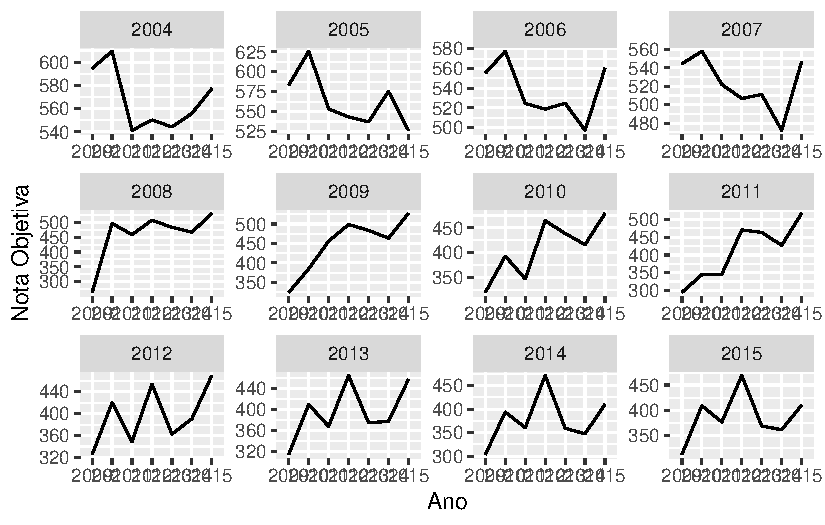
\includegraphics{script_files/figure-latex/unnamed-chunk-11-2.pdf}

\begin{Shaded}
\begin{Highlighting}[]
\NormalTok{dados\_ice\_v3 }\SpecialCharTok{\%\textgreater{}\%}
  \FunctionTok{filter}\NormalTok{(ano\_enem }\SpecialCharTok{\textgreater{}=} \DecValTok{2009}\NormalTok{, tratado }\SpecialCharTok{==} \DecValTok{1}\NormalTok{) }\SpecialCharTok{\%\textgreater{}\%}
  \FunctionTok{mutate}\NormalTok{(}\AttributeTok{ano\_enem =} \FunctionTok{as.factor}\NormalTok{(ano\_enem), }\AttributeTok{ano\_ice =} \FunctionTok{as.factor}\NormalTok{(ano\_ice)) }\SpecialCharTok{\%\textgreater{}\%}
  \FunctionTok{group\_by}\NormalTok{(ano\_enem, ano\_ice) }\SpecialCharTok{\%\textgreater{}\%}
  \FunctionTok{summarise}\NormalTok{(}
    \AttributeTok{enem\_nota\_redacao =} \FunctionTok{mean}\NormalTok{(enem\_nota\_redacao, }\AttributeTok{na.rm =} \ConstantTok{TRUE}\NormalTok{),}
    \AttributeTok{enem\_nota\_matematica =} \FunctionTok{mean}\NormalTok{(enem\_nota\_matematica, }\AttributeTok{na.rm =} \ConstantTok{TRUE}\NormalTok{),}
    \AttributeTok{enem\_nota\_linguagens =} \FunctionTok{mean}\NormalTok{(enem\_nota\_linguagens, }\AttributeTok{na.rm =} \ConstantTok{TRUE}\NormalTok{),}
    \AttributeTok{enem\_nota\_ciencias =} \FunctionTok{mean}\NormalTok{(enem\_nota\_ciencias, }\AttributeTok{na.rm =} \ConstantTok{TRUE}\NormalTok{),}
    \AttributeTok{enem\_nota\_humanas =} \FunctionTok{mean}\NormalTok{(enem\_nota\_humanas, }\AttributeTok{na.rm =} \ConstantTok{TRUE}\NormalTok{),}
    \AttributeTok{enem\_nota\_objetiva =} \FunctionTok{mean}\NormalTok{(enem\_nota\_objetivab, }\AttributeTok{na.rm =} \ConstantTok{TRUE}\NormalTok{),}
    \AttributeTok{.groups =} \StringTok{"drop"}  \CommentTok{\# Override grouping}
\NormalTok{  ) }\SpecialCharTok{\%\textgreater{}\%}
  \FunctionTok{ungroup}\NormalTok{() }\SpecialCharTok{\%\textgreater{}\%}
  \FunctionTok{pivot\_longer}\NormalTok{(}
    \SpecialCharTok{!}\FunctionTok{c}\NormalTok{(ano\_enem, ano\_ice),}
    \AttributeTok{names\_to =} \StringTok{\textquotesingle{}prova\textquotesingle{}}\NormalTok{,}
    \AttributeTok{values\_to =} \StringTok{\textquotesingle{}nota\textquotesingle{}}
\NormalTok{  ) }\SpecialCharTok{\%\textgreater{}\%}
  \FunctionTok{mutate}\NormalTok{(}
    \AttributeTok{prova =} \FunctionTok{case\_when}\NormalTok{(}
\NormalTok{      prova }\SpecialCharTok{==} \StringTok{\textquotesingle{}enem\_nota\_objetiva\textquotesingle{}} \SpecialCharTok{\textasciitilde{}} \StringTok{\textquotesingle{}Objetiva\textquotesingle{}}\NormalTok{,}
\NormalTok{      prova }\SpecialCharTok{==} \StringTok{\textquotesingle{}enem\_nota\_redacao\textquotesingle{}} \SpecialCharTok{\textasciitilde{}} \StringTok{\textquotesingle{}Redação\textquotesingle{}}\NormalTok{,}
\NormalTok{      prova }\SpecialCharTok{==} \StringTok{\textquotesingle{}enem\_nota\_matematica\textquotesingle{}} \SpecialCharTok{\textasciitilde{}} \StringTok{\textquotesingle{}Matemática\textquotesingle{}}\NormalTok{,}
\NormalTok{      prova }\SpecialCharTok{==} \StringTok{\textquotesingle{}enem\_nota\_linguagens\textquotesingle{}} \SpecialCharTok{\textasciitilde{}} \StringTok{\textquotesingle{}Linguagens\textquotesingle{}}\NormalTok{,}
\NormalTok{      prova }\SpecialCharTok{==} \StringTok{\textquotesingle{}enem\_nota\_humanas\textquotesingle{}} \SpecialCharTok{\textasciitilde{}} \StringTok{\textquotesingle{}Ciências Humanas\textquotesingle{}}\NormalTok{,}
\NormalTok{      prova }\SpecialCharTok{==} \StringTok{\textquotesingle{}enem\_nota\_ciencias\textquotesingle{}} \SpecialCharTok{\textasciitilde{}} \StringTok{\textquotesingle{}Ciências Naturais\textquotesingle{}}\NormalTok{,}
      \ConstantTok{TRUE} \SpecialCharTok{\textasciitilde{}}\NormalTok{ prova}
\NormalTok{    )}
\NormalTok{  ) }\SpecialCharTok{\%\textgreater{}\%}
  \FunctionTok{filter}\NormalTok{(prova }\SpecialCharTok{==} \StringTok{\textquotesingle{}Matemática\textquotesingle{}}\NormalTok{) }\SpecialCharTok{\%\textgreater{}\%} 
  \FunctionTok{ggplot}\NormalTok{() }\SpecialCharTok{+}
  \FunctionTok{geom\_line}\NormalTok{(}\FunctionTok{aes}\NormalTok{(ano\_enem, nota, }\AttributeTok{group =}\NormalTok{ ano\_ice)) }\SpecialCharTok{+}
  \FunctionTok{labs}\NormalTok{(}\AttributeTok{x =} \StringTok{\textquotesingle{}Ano\textquotesingle{}}\NormalTok{, }\AttributeTok{y =} \StringTok{\textquotesingle{}Nota Matemática\textquotesingle{}}\NormalTok{) }\SpecialCharTok{+}
  \FunctionTok{facet\_wrap}\NormalTok{(}\FunctionTok{vars}\NormalTok{(ano\_ice), }\AttributeTok{scales =} \StringTok{"free"}\NormalTok{)}
\end{Highlighting}
\end{Shaded}

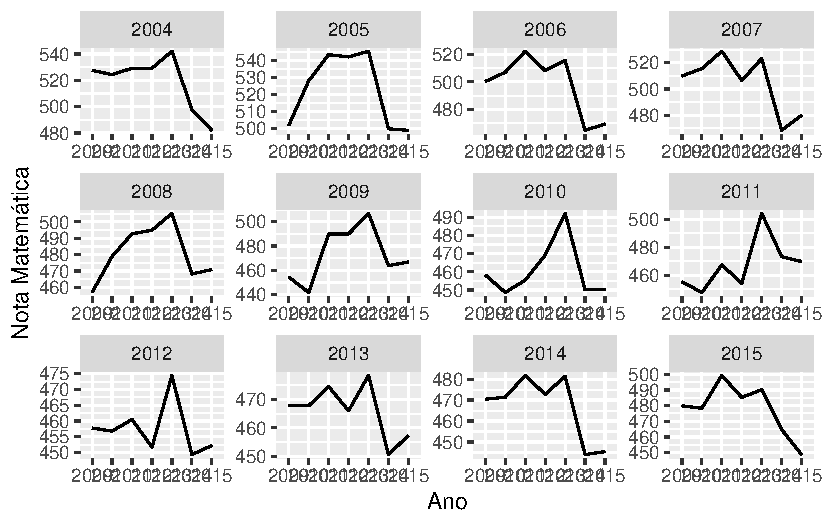
\includegraphics{script_files/figure-latex/unnamed-chunk-11-3.pdf}

\begin{Shaded}
\begin{Highlighting}[]
\NormalTok{dados\_ice\_v3 }\SpecialCharTok{\%\textgreater{}\%}
  \FunctionTok{filter}\NormalTok{(ano\_enem }\SpecialCharTok{\textgreater{}=} \DecValTok{2009}\NormalTok{, tratado }\SpecialCharTok{==} \DecValTok{1}\NormalTok{) }\SpecialCharTok{\%\textgreater{}\%}
  \FunctionTok{mutate}\NormalTok{(}\AttributeTok{ano\_enem =} \FunctionTok{as.factor}\NormalTok{(ano\_enem), }\AttributeTok{ano\_ice =} \FunctionTok{as.factor}\NormalTok{(ano\_ice)) }\SpecialCharTok{\%\textgreater{}\%}
  \FunctionTok{group\_by}\NormalTok{(ano\_enem, ano\_ice) }\SpecialCharTok{\%\textgreater{}\%}
  \FunctionTok{summarise}\NormalTok{(}
    \AttributeTok{enem\_nota\_redacao =} \FunctionTok{mean}\NormalTok{(enem\_nota\_redacao, }\AttributeTok{na.rm =} \ConstantTok{TRUE}\NormalTok{),}
    \AttributeTok{enem\_nota\_matematica =} \FunctionTok{mean}\NormalTok{(enem\_nota\_matematica, }\AttributeTok{na.rm =} \ConstantTok{TRUE}\NormalTok{),}
    \AttributeTok{enem\_nota\_linguagens =} \FunctionTok{mean}\NormalTok{(enem\_nota\_linguagens, }\AttributeTok{na.rm =} \ConstantTok{TRUE}\NormalTok{),}
    \AttributeTok{enem\_nota\_ciencias =} \FunctionTok{mean}\NormalTok{(enem\_nota\_ciencias, }\AttributeTok{na.rm =} \ConstantTok{TRUE}\NormalTok{),}
    \AttributeTok{enem\_nota\_humanas =} \FunctionTok{mean}\NormalTok{(enem\_nota\_humanas, }\AttributeTok{na.rm =} \ConstantTok{TRUE}\NormalTok{),}
    \AttributeTok{enem\_nota\_objetiva =} \FunctionTok{mean}\NormalTok{(enem\_nota\_objetivab, }\AttributeTok{na.rm =} \ConstantTok{TRUE}\NormalTok{),}
    \AttributeTok{.groups =} \StringTok{"drop"}  \CommentTok{\# Override grouping}
\NormalTok{  ) }\SpecialCharTok{\%\textgreater{}\%}
  \FunctionTok{ungroup}\NormalTok{() }\SpecialCharTok{\%\textgreater{}\%}
  \FunctionTok{pivot\_longer}\NormalTok{(}
    \SpecialCharTok{!}\FunctionTok{c}\NormalTok{(ano\_enem, ano\_ice),}
    \AttributeTok{names\_to =} \StringTok{\textquotesingle{}prova\textquotesingle{}}\NormalTok{,}
    \AttributeTok{values\_to =} \StringTok{\textquotesingle{}nota\textquotesingle{}}
\NormalTok{  ) }\SpecialCharTok{\%\textgreater{}\%}
  \FunctionTok{mutate}\NormalTok{(}
    \AttributeTok{prova =} \FunctionTok{case\_when}\NormalTok{(}
\NormalTok{      prova }\SpecialCharTok{==} \StringTok{\textquotesingle{}enem\_nota\_objetiva\textquotesingle{}} \SpecialCharTok{\textasciitilde{}} \StringTok{\textquotesingle{}Objetiva\textquotesingle{}}\NormalTok{,}
\NormalTok{      prova }\SpecialCharTok{==} \StringTok{\textquotesingle{}enem\_nota\_redacao\textquotesingle{}} \SpecialCharTok{\textasciitilde{}} \StringTok{\textquotesingle{}Redação\textquotesingle{}}\NormalTok{,}
\NormalTok{      prova }\SpecialCharTok{==} \StringTok{\textquotesingle{}enem\_nota\_matematica\textquotesingle{}} \SpecialCharTok{\textasciitilde{}} \StringTok{\textquotesingle{}Matemática\textquotesingle{}}\NormalTok{,}
\NormalTok{      prova }\SpecialCharTok{==} \StringTok{\textquotesingle{}enem\_nota\_linguagens\textquotesingle{}} \SpecialCharTok{\textasciitilde{}} \StringTok{\textquotesingle{}Linguagens\textquotesingle{}}\NormalTok{,}
\NormalTok{      prova }\SpecialCharTok{==} \StringTok{\textquotesingle{}enem\_nota\_humanas\textquotesingle{}} \SpecialCharTok{\textasciitilde{}} \StringTok{\textquotesingle{}Ciências Humanas\textquotesingle{}}\NormalTok{,}
\NormalTok{      prova }\SpecialCharTok{==} \StringTok{\textquotesingle{}enem\_nota\_ciencias\textquotesingle{}} \SpecialCharTok{\textasciitilde{}} \StringTok{\textquotesingle{}Ciências Naturais\textquotesingle{}}\NormalTok{,}
      \ConstantTok{TRUE} \SpecialCharTok{\textasciitilde{}}\NormalTok{ prova}
\NormalTok{    )}
\NormalTok{  ) }\SpecialCharTok{\%\textgreater{}\%}
  \FunctionTok{filter}\NormalTok{(prova }\SpecialCharTok{==} \StringTok{\textquotesingle{}Linguagens\textquotesingle{}}\NormalTok{) }\SpecialCharTok{\%\textgreater{}\%} 
  \FunctionTok{ggplot}\NormalTok{() }\SpecialCharTok{+}
  \FunctionTok{geom\_line}\NormalTok{(}\FunctionTok{aes}\NormalTok{(ano\_enem, nota, }\AttributeTok{group =}\NormalTok{ ano\_ice)) }\SpecialCharTok{+}
  \FunctionTok{labs}\NormalTok{(}\AttributeTok{x =} \StringTok{\textquotesingle{}Ano\textquotesingle{}}\NormalTok{, }\AttributeTok{y =} \StringTok{\textquotesingle{}Nota Linguagens\textquotesingle{}}\NormalTok{) }\SpecialCharTok{+}
  \FunctionTok{facet\_wrap}\NormalTok{(}\FunctionTok{vars}\NormalTok{(ano\_ice), }\AttributeTok{scales =} \StringTok{"free"}\NormalTok{)}
\end{Highlighting}
\end{Shaded}

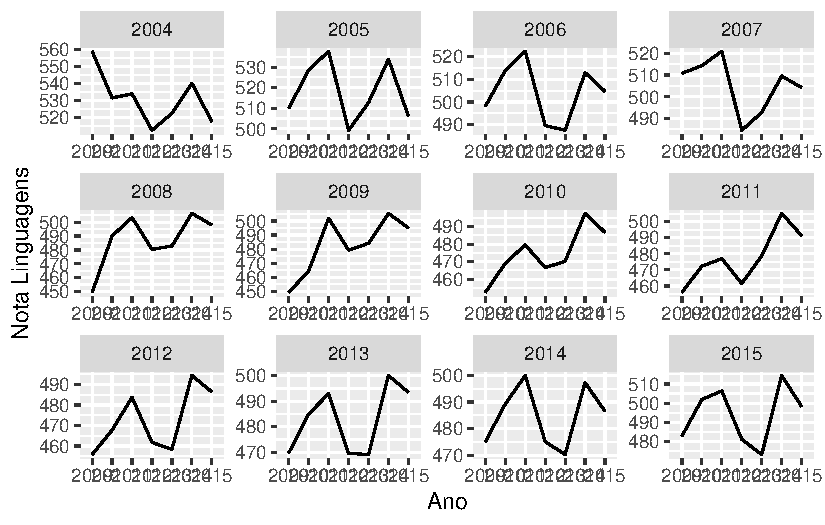
\includegraphics{script_files/figure-latex/unnamed-chunk-11-4.pdf}

\begin{Shaded}
\begin{Highlighting}[]
\NormalTok{dados\_ice\_v3 }\SpecialCharTok{\%\textgreater{}\%}
  \FunctionTok{filter}\NormalTok{(ano\_enem }\SpecialCharTok{\textgreater{}=} \DecValTok{2009}\NormalTok{, tratado }\SpecialCharTok{==} \DecValTok{1}\NormalTok{) }\SpecialCharTok{\%\textgreater{}\%}
  \FunctionTok{mutate}\NormalTok{(}\AttributeTok{ano\_enem =} \FunctionTok{as.factor}\NormalTok{(ano\_enem), }\AttributeTok{ano\_ice =} \FunctionTok{as.factor}\NormalTok{(ano\_ice)) }\SpecialCharTok{\%\textgreater{}\%}
  \FunctionTok{group\_by}\NormalTok{(ano\_enem, ano\_ice) }\SpecialCharTok{\%\textgreater{}\%}
  \FunctionTok{summarise}\NormalTok{(}
    \AttributeTok{enem\_nota\_redacao =} \FunctionTok{mean}\NormalTok{(enem\_nota\_redacao, }\AttributeTok{na.rm =} \ConstantTok{TRUE}\NormalTok{),}
    \AttributeTok{enem\_nota\_matematica =} \FunctionTok{mean}\NormalTok{(enem\_nota\_matematica, }\AttributeTok{na.rm =} \ConstantTok{TRUE}\NormalTok{),}
    \AttributeTok{enem\_nota\_linguagens =} \FunctionTok{mean}\NormalTok{(enem\_nota\_linguagens, }\AttributeTok{na.rm =} \ConstantTok{TRUE}\NormalTok{),}
    \AttributeTok{enem\_nota\_ciencias =} \FunctionTok{mean}\NormalTok{(enem\_nota\_ciencias, }\AttributeTok{na.rm =} \ConstantTok{TRUE}\NormalTok{),}
    \AttributeTok{enem\_nota\_humanas =} \FunctionTok{mean}\NormalTok{(enem\_nota\_humanas, }\AttributeTok{na.rm =} \ConstantTok{TRUE}\NormalTok{),}
    \AttributeTok{enem\_nota\_objetiva =} \FunctionTok{mean}\NormalTok{(enem\_nota\_objetivab, }\AttributeTok{na.rm =} \ConstantTok{TRUE}\NormalTok{),}
    \AttributeTok{.groups =} \StringTok{"drop"}  \CommentTok{\# Override grouping}
\NormalTok{  ) }\SpecialCharTok{\%\textgreater{}\%}
  \FunctionTok{ungroup}\NormalTok{() }\SpecialCharTok{\%\textgreater{}\%}
  \FunctionTok{pivot\_longer}\NormalTok{(}
    \SpecialCharTok{!}\FunctionTok{c}\NormalTok{(ano\_enem, ano\_ice),}
    \AttributeTok{names\_to =} \StringTok{\textquotesingle{}prova\textquotesingle{}}\NormalTok{,}
    \AttributeTok{values\_to =} \StringTok{\textquotesingle{}nota\textquotesingle{}}
\NormalTok{  ) }\SpecialCharTok{\%\textgreater{}\%}
  \FunctionTok{mutate}\NormalTok{(}
    \AttributeTok{prova =} \FunctionTok{case\_when}\NormalTok{(}
\NormalTok{      prova }\SpecialCharTok{==} \StringTok{\textquotesingle{}enem\_nota\_objetiva\textquotesingle{}} \SpecialCharTok{\textasciitilde{}} \StringTok{\textquotesingle{}Objetiva\textquotesingle{}}\NormalTok{,}
\NormalTok{      prova }\SpecialCharTok{==} \StringTok{\textquotesingle{}enem\_nota\_redacao\textquotesingle{}} \SpecialCharTok{\textasciitilde{}} \StringTok{\textquotesingle{}Redação\textquotesingle{}}\NormalTok{,}
\NormalTok{      prova }\SpecialCharTok{==} \StringTok{\textquotesingle{}enem\_nota\_matematica\textquotesingle{}} \SpecialCharTok{\textasciitilde{}} \StringTok{\textquotesingle{}Matemática\textquotesingle{}}\NormalTok{,}
\NormalTok{      prova }\SpecialCharTok{==} \StringTok{\textquotesingle{}enem\_nota\_linguagens\textquotesingle{}} \SpecialCharTok{\textasciitilde{}} \StringTok{\textquotesingle{}Linguagens\textquotesingle{}}\NormalTok{,}
\NormalTok{      prova }\SpecialCharTok{==} \StringTok{\textquotesingle{}enem\_nota\_humanas\textquotesingle{}} \SpecialCharTok{\textasciitilde{}} \StringTok{\textquotesingle{}Ciências Humanas\textquotesingle{}}\NormalTok{,}
\NormalTok{      prova }\SpecialCharTok{==} \StringTok{\textquotesingle{}enem\_nota\_ciencias\textquotesingle{}} \SpecialCharTok{\textasciitilde{}} \StringTok{\textquotesingle{}Ciências Naturais\textquotesingle{}}\NormalTok{,}
      \ConstantTok{TRUE} \SpecialCharTok{\textasciitilde{}}\NormalTok{ prova}
\NormalTok{    )}
\NormalTok{  ) }\SpecialCharTok{\%\textgreater{}\%}
  \FunctionTok{filter}\NormalTok{(prova }\SpecialCharTok{==} \StringTok{\textquotesingle{}Ciências Humanas\textquotesingle{}}\NormalTok{) }\SpecialCharTok{\%\textgreater{}\%} 
  \FunctionTok{ggplot}\NormalTok{() }\SpecialCharTok{+}
  \FunctionTok{geom\_line}\NormalTok{(}\FunctionTok{aes}\NormalTok{(ano\_enem, nota, }\AttributeTok{group =}\NormalTok{ ano\_ice)) }\SpecialCharTok{+}
  \FunctionTok{labs}\NormalTok{(}\AttributeTok{x =} \StringTok{\textquotesingle{}Ano\textquotesingle{}}\NormalTok{, }\AttributeTok{y =} \StringTok{\textquotesingle{}Nota Ciências Humanas\textquotesingle{}}\NormalTok{) }\SpecialCharTok{+}
  \FunctionTok{facet\_wrap}\NormalTok{(}\FunctionTok{vars}\NormalTok{(ano\_ice), }\AttributeTok{scales =} \StringTok{"free"}\NormalTok{)}
\end{Highlighting}
\end{Shaded}

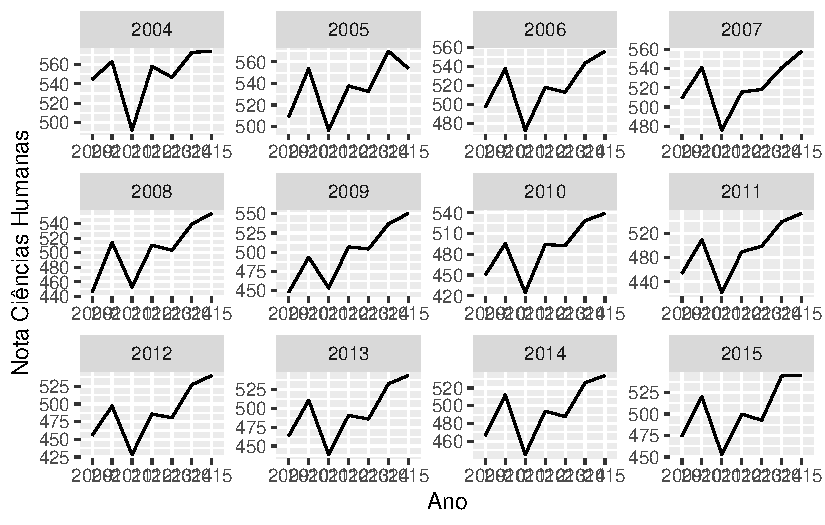
\includegraphics{script_files/figure-latex/unnamed-chunk-11-5.pdf}

\begin{Shaded}
\begin{Highlighting}[]
\NormalTok{dados\_ice\_v3 }\SpecialCharTok{\%\textgreater{}\%}
  \FunctionTok{filter}\NormalTok{(ano\_enem }\SpecialCharTok{\textgreater{}=} \DecValTok{2009}\NormalTok{, tratado }\SpecialCharTok{==} \DecValTok{1}\NormalTok{) }\SpecialCharTok{\%\textgreater{}\%}
  \FunctionTok{mutate}\NormalTok{(}\AttributeTok{ano\_enem =} \FunctionTok{as.factor}\NormalTok{(ano\_enem), }\AttributeTok{ano\_ice =} \FunctionTok{as.factor}\NormalTok{(ano\_ice)) }\SpecialCharTok{\%\textgreater{}\%}
  \FunctionTok{group\_by}\NormalTok{(ano\_enem, ano\_ice) }\SpecialCharTok{\%\textgreater{}\%}
  \FunctionTok{summarise}\NormalTok{(}
    \AttributeTok{enem\_nota\_redacao =} \FunctionTok{mean}\NormalTok{(enem\_nota\_redacao, }\AttributeTok{na.rm =} \ConstantTok{TRUE}\NormalTok{),}
    \AttributeTok{enem\_nota\_matematica =} \FunctionTok{mean}\NormalTok{(enem\_nota\_matematica, }\AttributeTok{na.rm =} \ConstantTok{TRUE}\NormalTok{),}
    \AttributeTok{enem\_nota\_linguagens =} \FunctionTok{mean}\NormalTok{(enem\_nota\_linguagens, }\AttributeTok{na.rm =} \ConstantTok{TRUE}\NormalTok{),}
    \AttributeTok{enem\_nota\_ciencias =} \FunctionTok{mean}\NormalTok{(enem\_nota\_ciencias, }\AttributeTok{na.rm =} \ConstantTok{TRUE}\NormalTok{),}
    \AttributeTok{enem\_nota\_humanas =} \FunctionTok{mean}\NormalTok{(enem\_nota\_humanas, }\AttributeTok{na.rm =} \ConstantTok{TRUE}\NormalTok{),}
    \AttributeTok{enem\_nota\_objetiva =} \FunctionTok{mean}\NormalTok{(enem\_nota\_objetivab, }\AttributeTok{na.rm =} \ConstantTok{TRUE}\NormalTok{),}
    \AttributeTok{.groups =} \StringTok{"drop"}  \CommentTok{\# Override grouping}
\NormalTok{  ) }\SpecialCharTok{\%\textgreater{}\%}
  \FunctionTok{ungroup}\NormalTok{() }\SpecialCharTok{\%\textgreater{}\%}
  \FunctionTok{pivot\_longer}\NormalTok{(}
    \SpecialCharTok{!}\FunctionTok{c}\NormalTok{(ano\_enem, ano\_ice),}
    \AttributeTok{names\_to =} \StringTok{\textquotesingle{}prova\textquotesingle{}}\NormalTok{,}
    \AttributeTok{values\_to =} \StringTok{\textquotesingle{}nota\textquotesingle{}}
\NormalTok{  ) }\SpecialCharTok{\%\textgreater{}\%}
  \FunctionTok{mutate}\NormalTok{(}
    \AttributeTok{prova =} \FunctionTok{case\_when}\NormalTok{(}
\NormalTok{      prova }\SpecialCharTok{==} \StringTok{\textquotesingle{}enem\_nota\_objetiva\textquotesingle{}} \SpecialCharTok{\textasciitilde{}} \StringTok{\textquotesingle{}Objetiva\textquotesingle{}}\NormalTok{,}
\NormalTok{      prova }\SpecialCharTok{==} \StringTok{\textquotesingle{}enem\_nota\_redacao\textquotesingle{}} \SpecialCharTok{\textasciitilde{}} \StringTok{\textquotesingle{}Redação\textquotesingle{}}\NormalTok{,}
\NormalTok{      prova }\SpecialCharTok{==} \StringTok{\textquotesingle{}enem\_nota\_matematica\textquotesingle{}} \SpecialCharTok{\textasciitilde{}} \StringTok{\textquotesingle{}Matemática\textquotesingle{}}\NormalTok{,}
\NormalTok{      prova }\SpecialCharTok{==} \StringTok{\textquotesingle{}enem\_nota\_linguagens\textquotesingle{}} \SpecialCharTok{\textasciitilde{}} \StringTok{\textquotesingle{}Linguagens\textquotesingle{}}\NormalTok{,}
\NormalTok{      prova }\SpecialCharTok{==} \StringTok{\textquotesingle{}enem\_nota\_humanas\textquotesingle{}} \SpecialCharTok{\textasciitilde{}} \StringTok{\textquotesingle{}Ciências Humanas\textquotesingle{}}\NormalTok{,}
\NormalTok{      prova }\SpecialCharTok{==} \StringTok{\textquotesingle{}enem\_nota\_ciencias\textquotesingle{}} \SpecialCharTok{\textasciitilde{}} \StringTok{\textquotesingle{}Ciências Naturais\textquotesingle{}}\NormalTok{,}
      \ConstantTok{TRUE} \SpecialCharTok{\textasciitilde{}}\NormalTok{ prova}
\NormalTok{    )}
\NormalTok{  ) }\SpecialCharTok{\%\textgreater{}\%}
  \FunctionTok{filter}\NormalTok{(prova }\SpecialCharTok{==} \StringTok{\textquotesingle{}Ciências Naturais\textquotesingle{}}\NormalTok{) }\SpecialCharTok{\%\textgreater{}\%} 
  \FunctionTok{ggplot}\NormalTok{() }\SpecialCharTok{+}
  \FunctionTok{geom\_line}\NormalTok{(}\FunctionTok{aes}\NormalTok{(ano\_enem, nota, }\AttributeTok{group =}\NormalTok{ ano\_ice)) }\SpecialCharTok{+}
  \FunctionTok{labs}\NormalTok{(}\AttributeTok{x =} \StringTok{\textquotesingle{}Ano\textquotesingle{}}\NormalTok{, }\AttributeTok{y =} \StringTok{\textquotesingle{}Nota Ciências Naturais\textquotesingle{}}\NormalTok{) }\SpecialCharTok{+}
  \FunctionTok{facet\_wrap}\NormalTok{(}\FunctionTok{vars}\NormalTok{(ano\_ice), }\AttributeTok{scales =} \StringTok{"free"}\NormalTok{)}
\end{Highlighting}
\end{Shaded}

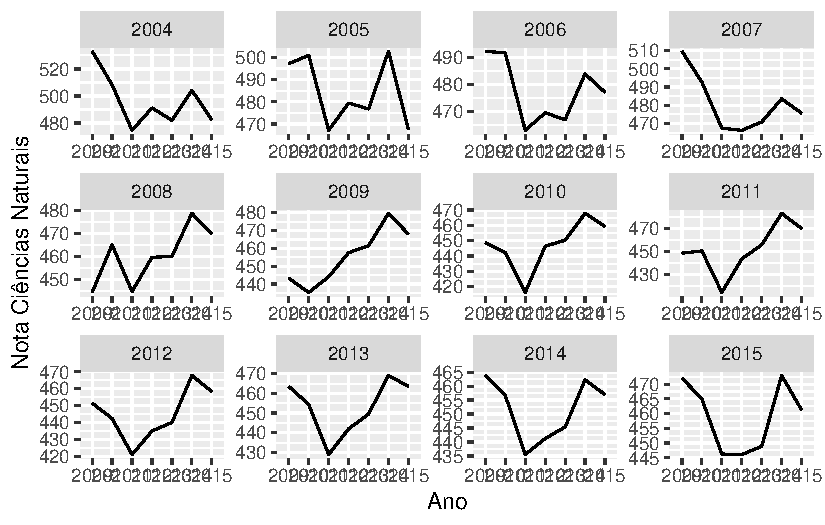
\includegraphics{script_files/figure-latex/unnamed-chunk-11-6.pdf}

\begin{Shaded}
\begin{Highlighting}[]
\NormalTok{painel\_indicadores\_simplificado }\SpecialCharTok{\%\textgreater{}\%} 
  \FunctionTok{filter}\NormalTok{(tratado }\SpecialCharTok{==} \DecValTok{1}\NormalTok{) }\SpecialCharTok{\%\textgreater{}\%} 
  \FunctionTok{mutate}\NormalTok{(}\AttributeTok{ano\_censo =} \FunctionTok{as.factor}\NormalTok{(ano\_censo.x),}
         \AttributeTok{ano\_ice =} \FunctionTok{as.factor}\NormalTok{(ano\_ice)) }\SpecialCharTok{\%\textgreater{}\%} 
  \FunctionTok{group\_by}\NormalTok{(ano\_censo,ano\_ice) }\SpecialCharTok{\%\textgreater{}\%} 
  \FunctionTok{summarise}\NormalTok{(}\AttributeTok{aprovacao =} \FunctionTok{mean}\NormalTok{(apr\_em, }\AttributeTok{na.rm =}\NormalTok{ T),}
            \AttributeTok{reprovacao =} \FunctionTok{mean}\NormalTok{(rep\_em, }\AttributeTok{na.rm =}\NormalTok{ T),}
            \AttributeTok{abandono =} \FunctionTok{mean}\NormalTok{(aba\_em, }\AttributeTok{na.rm =}\NormalTok{ T),}
            \AttributeTok{distorcao =} \FunctionTok{mean}\NormalTok{(dist\_em, }\AttributeTok{na.rm =}\NormalTok{ T),}
            \AttributeTok{.groups =} \StringTok{"drop"}  \CommentTok{\# Override grouping}
\NormalTok{            ) }\SpecialCharTok{\%\textgreater{}\%}
\FunctionTok{pivot\_longer}\NormalTok{(}\SpecialCharTok{!}\FunctionTok{c}\NormalTok{(ano\_censo,ano\_ice), }
             \AttributeTok{names\_to =} \StringTok{\textquotesingle{}prova\textquotesingle{}}\NormalTok{,}
             \AttributeTok{values\_to =} \StringTok{\textquotesingle{}nota\textquotesingle{}}\NormalTok{) }\SpecialCharTok{\%\textgreater{}\%} 
  \FunctionTok{mutate}\NormalTok{(}\AttributeTok{prova =} \FunctionTok{case\_when}\NormalTok{(prova }\SpecialCharTok{==} \StringTok{\textquotesingle{}aprovacao\textquotesingle{}} \SpecialCharTok{\textasciitilde{}} \StringTok{\textquotesingle{}Aprovação\textquotesingle{}}\NormalTok{,}
\NormalTok{                         prova }\SpecialCharTok{==} \StringTok{\textquotesingle{}reprovacao\textquotesingle{}} \SpecialCharTok{\textasciitilde{}} \StringTok{\textquotesingle{}Reprovação\textquotesingle{}}\NormalTok{,}
\NormalTok{                         prova }\SpecialCharTok{==} \StringTok{\textquotesingle{}abandono\textquotesingle{}} \SpecialCharTok{\textasciitilde{}} \StringTok{\textquotesingle{}Abandono\textquotesingle{}}\NormalTok{,}
\NormalTok{                         prova }\SpecialCharTok{==} \StringTok{\textquotesingle{}distorcao\textquotesingle{}} \SpecialCharTok{\textasciitilde{}} \StringTok{\textquotesingle{}Distorção\textquotesingle{}}\NormalTok{,}
\NormalTok{                         T }\SpecialCharTok{\textasciitilde{}}\NormalTok{ prova)) }\SpecialCharTok{\%\textgreater{}\%} 
  \FunctionTok{filter}\NormalTok{(prova }\SpecialCharTok{==} \StringTok{\textquotesingle{}Aprovação\textquotesingle{}}\NormalTok{) }\SpecialCharTok{\%\textgreater{}\%} 
  \FunctionTok{ggplot}\NormalTok{() }\SpecialCharTok{+}
  \FunctionTok{geom\_line}\NormalTok{(}\FunctionTok{aes}\NormalTok{(ano\_censo, nota, }\AttributeTok{group =}\NormalTok{ ano\_ice)) }\SpecialCharTok{+}
  \FunctionTok{labs}\NormalTok{(}\AttributeTok{x =} \StringTok{\textquotesingle{}Ano\textquotesingle{}}\NormalTok{, }\AttributeTok{y =} \StringTok{\textquotesingle{}Taxa de Aprovação (\%)\textquotesingle{}}\NormalTok{) }\SpecialCharTok{+}
  \FunctionTok{facet\_wrap}\NormalTok{(}\FunctionTok{vars}\NormalTok{(ano\_ice), }\AttributeTok{scales =} \StringTok{"free"}\NormalTok{)}
\end{Highlighting}
\end{Shaded}

\begin{verbatim}
Warning: Removed 18 rows containing missing values or values outside the scale range
(`geom_line()`).
\end{verbatim}

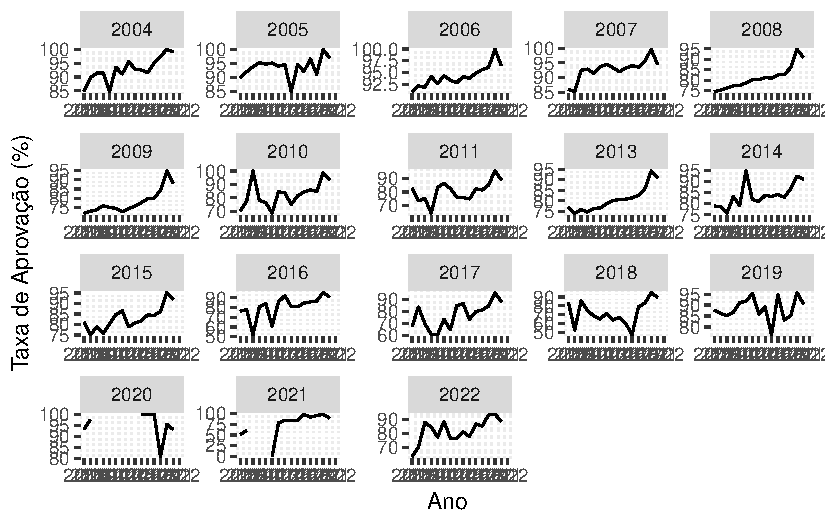
\includegraphics{script_files/figure-latex/unnamed-chunk-12-1.pdf}

\begin{Shaded}
\begin{Highlighting}[]
\NormalTok{painel\_indicadores\_simplificado }\SpecialCharTok{\%\textgreater{}\%} 
  \FunctionTok{filter}\NormalTok{(tratado }\SpecialCharTok{==} \DecValTok{1}\NormalTok{) }\SpecialCharTok{\%\textgreater{}\%} 
  \FunctionTok{mutate}\NormalTok{(}\AttributeTok{ano\_censo =} \FunctionTok{as.factor}\NormalTok{(ano\_censo.x),}
         \AttributeTok{ano\_ice =} \FunctionTok{as.factor}\NormalTok{(ano\_ice)) }\SpecialCharTok{\%\textgreater{}\%} 
  \FunctionTok{group\_by}\NormalTok{(ano\_censo,ano\_ice) }\SpecialCharTok{\%\textgreater{}\%} 
  \FunctionTok{summarise}\NormalTok{(}\AttributeTok{aprovacao =} \FunctionTok{mean}\NormalTok{(apr\_em, }\AttributeTok{na.rm =}\NormalTok{ T),}
            \AttributeTok{reprovacao =} \FunctionTok{mean}\NormalTok{(rep\_em, }\AttributeTok{na.rm =}\NormalTok{ T),}
            \AttributeTok{abandono =} \FunctionTok{mean}\NormalTok{(aba\_em, }\AttributeTok{na.rm =}\NormalTok{ T),}
            \AttributeTok{distorcao =} \FunctionTok{mean}\NormalTok{(dist\_em, }\AttributeTok{na.rm =}\NormalTok{ T),}
            \AttributeTok{.groups =} \StringTok{"drop"}  \CommentTok{\# Override grouping}
\NormalTok{            ) }\SpecialCharTok{\%\textgreater{}\%}
\FunctionTok{pivot\_longer}\NormalTok{(}\SpecialCharTok{!}\FunctionTok{c}\NormalTok{(ano\_censo,ano\_ice), }
             \AttributeTok{names\_to =} \StringTok{\textquotesingle{}prova\textquotesingle{}}\NormalTok{,}
             \AttributeTok{values\_to =} \StringTok{\textquotesingle{}nota\textquotesingle{}}\NormalTok{) }\SpecialCharTok{\%\textgreater{}\%} 
  \FunctionTok{mutate}\NormalTok{(}\AttributeTok{prova =} \FunctionTok{case\_when}\NormalTok{(prova }\SpecialCharTok{==} \StringTok{\textquotesingle{}aprovacao\textquotesingle{}} \SpecialCharTok{\textasciitilde{}} \StringTok{\textquotesingle{}Aprovação\textquotesingle{}}\NormalTok{,}
\NormalTok{                         prova }\SpecialCharTok{==} \StringTok{\textquotesingle{}reprovacao\textquotesingle{}} \SpecialCharTok{\textasciitilde{}} \StringTok{\textquotesingle{}Reprovação\textquotesingle{}}\NormalTok{,}
\NormalTok{                         prova }\SpecialCharTok{==} \StringTok{\textquotesingle{}abandono\textquotesingle{}} \SpecialCharTok{\textasciitilde{}} \StringTok{\textquotesingle{}Abandono\textquotesingle{}}\NormalTok{,}
\NormalTok{                         prova }\SpecialCharTok{==} \StringTok{\textquotesingle{}distorcao\textquotesingle{}} \SpecialCharTok{\textasciitilde{}} \StringTok{\textquotesingle{}Distorção\textquotesingle{}}\NormalTok{,}
\NormalTok{                         T }\SpecialCharTok{\textasciitilde{}}\NormalTok{ prova)) }\SpecialCharTok{\%\textgreater{}\%} 
  \FunctionTok{filter}\NormalTok{(prova }\SpecialCharTok{==} \StringTok{\textquotesingle{}Reprovação\textquotesingle{}}\NormalTok{) }\SpecialCharTok{\%\textgreater{}\%} 
  \FunctionTok{ggplot}\NormalTok{() }\SpecialCharTok{+}
  \FunctionTok{geom\_line}\NormalTok{(}\FunctionTok{aes}\NormalTok{(ano\_censo, nota, }\AttributeTok{group =}\NormalTok{ ano\_ice)) }\SpecialCharTok{+}
  \FunctionTok{labs}\NormalTok{(}\AttributeTok{x =} \StringTok{\textquotesingle{}Ano\textquotesingle{}}\NormalTok{, }\AttributeTok{y =} \StringTok{\textquotesingle{}Taxa de Reprovação (\%)\textquotesingle{}}\NormalTok{) }\SpecialCharTok{+}
  \FunctionTok{facet\_wrap}\NormalTok{(}\FunctionTok{vars}\NormalTok{(ano\_ice), }\AttributeTok{scales =} \StringTok{"free"}\NormalTok{)}
\end{Highlighting}
\end{Shaded}

\begin{verbatim}
Warning: Removed 18 rows containing missing values or values outside the scale range
(`geom_line()`).
\end{verbatim}

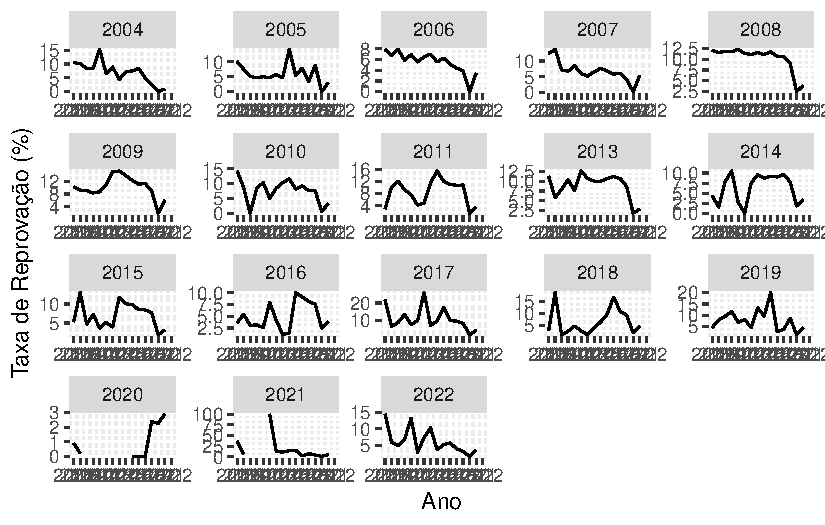
\includegraphics{script_files/figure-latex/unnamed-chunk-12-2.pdf}

\begin{Shaded}
\begin{Highlighting}[]
\NormalTok{painel\_indicadores\_simplificado }\SpecialCharTok{\%\textgreater{}\%} 
  \FunctionTok{filter}\NormalTok{(tratado }\SpecialCharTok{==} \DecValTok{1}\NormalTok{) }\SpecialCharTok{\%\textgreater{}\%} 
  \FunctionTok{mutate}\NormalTok{(}\AttributeTok{ano\_censo =} \FunctionTok{as.factor}\NormalTok{(ano\_censo.x),}
         \AttributeTok{ano\_ice =} \FunctionTok{as.factor}\NormalTok{(ano\_ice)) }\SpecialCharTok{\%\textgreater{}\%} 
  \FunctionTok{group\_by}\NormalTok{(ano\_censo,ano\_ice) }\SpecialCharTok{\%\textgreater{}\%} 
  \FunctionTok{summarise}\NormalTok{(}\AttributeTok{aprovacao =} \FunctionTok{mean}\NormalTok{(apr\_em, }\AttributeTok{na.rm =}\NormalTok{ T),}
            \AttributeTok{reprovacao =} \FunctionTok{mean}\NormalTok{(rep\_em, }\AttributeTok{na.rm =}\NormalTok{ T),}
            \AttributeTok{abandono =} \FunctionTok{mean}\NormalTok{(aba\_em, }\AttributeTok{na.rm =}\NormalTok{ T),}
            \AttributeTok{distorcao =} \FunctionTok{mean}\NormalTok{(dist\_em, }\AttributeTok{na.rm =}\NormalTok{ T),}
            \AttributeTok{.groups =} \StringTok{"drop"}  \CommentTok{\# Override grouping}
\NormalTok{            ) }\SpecialCharTok{\%\textgreater{}\%}
\FunctionTok{pivot\_longer}\NormalTok{(}\SpecialCharTok{!}\FunctionTok{c}\NormalTok{(ano\_censo,ano\_ice), }
             \AttributeTok{names\_to =} \StringTok{\textquotesingle{}prova\textquotesingle{}}\NormalTok{,}
             \AttributeTok{values\_to =} \StringTok{\textquotesingle{}nota\textquotesingle{}}\NormalTok{) }\SpecialCharTok{\%\textgreater{}\%} 
  \FunctionTok{mutate}\NormalTok{(}\AttributeTok{prova =} \FunctionTok{case\_when}\NormalTok{(prova }\SpecialCharTok{==} \StringTok{\textquotesingle{}aprovacao\textquotesingle{}} \SpecialCharTok{\textasciitilde{}} \StringTok{\textquotesingle{}Aprovação\textquotesingle{}}\NormalTok{,}
\NormalTok{                         prova }\SpecialCharTok{==} \StringTok{\textquotesingle{}reprovacao\textquotesingle{}} \SpecialCharTok{\textasciitilde{}} \StringTok{\textquotesingle{}Reprovação\textquotesingle{}}\NormalTok{,}
\NormalTok{                         prova }\SpecialCharTok{==} \StringTok{\textquotesingle{}abandono\textquotesingle{}} \SpecialCharTok{\textasciitilde{}} \StringTok{\textquotesingle{}Abandono\textquotesingle{}}\NormalTok{,}
\NormalTok{                         prova }\SpecialCharTok{==} \StringTok{\textquotesingle{}distorcao\textquotesingle{}} \SpecialCharTok{\textasciitilde{}} \StringTok{\textquotesingle{}Distorção\textquotesingle{}}\NormalTok{,}
\NormalTok{                         T }\SpecialCharTok{\textasciitilde{}}\NormalTok{ prova)) }\SpecialCharTok{\%\textgreater{}\%} 
  \FunctionTok{filter}\NormalTok{(prova }\SpecialCharTok{==} \StringTok{\textquotesingle{}Abandono\textquotesingle{}}\NormalTok{) }\SpecialCharTok{\%\textgreater{}\%} 
  \FunctionTok{ggplot}\NormalTok{() }\SpecialCharTok{+}
  \FunctionTok{geom\_line}\NormalTok{(}\FunctionTok{aes}\NormalTok{(ano\_censo, nota, }\AttributeTok{group =}\NormalTok{ ano\_ice)) }\SpecialCharTok{+}
  \FunctionTok{labs}\NormalTok{(}\AttributeTok{x =} \StringTok{\textquotesingle{}Ano\textquotesingle{}}\NormalTok{, }\AttributeTok{y =} \StringTok{\textquotesingle{}Taxa de Abandono (\%)\textquotesingle{}}\NormalTok{) }\SpecialCharTok{+}
  \FunctionTok{facet\_wrap}\NormalTok{(}\FunctionTok{vars}\NormalTok{(ano\_ice), }\AttributeTok{scales =} \StringTok{"free"}\NormalTok{)}
\end{Highlighting}
\end{Shaded}

\begin{verbatim}
Warning: Removed 18 rows containing missing values or values outside the scale range
(`geom_line()`).
\end{verbatim}

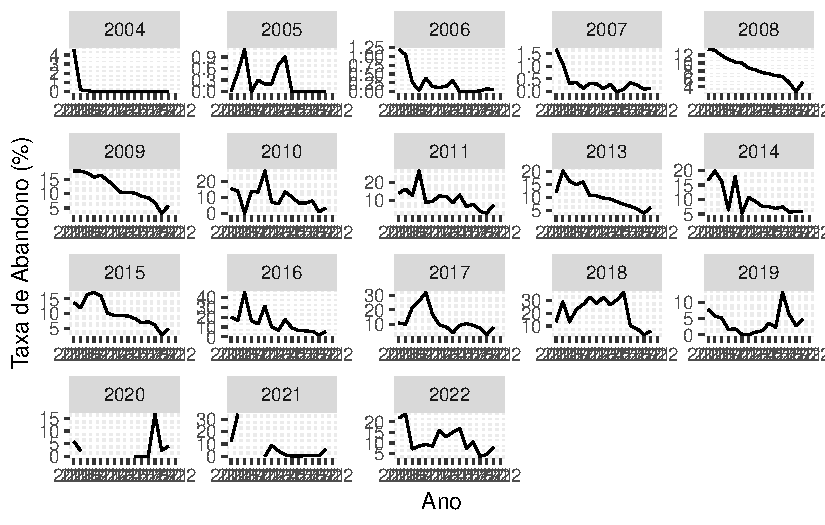
\includegraphics{script_files/figure-latex/unnamed-chunk-12-3.pdf}

\begin{Shaded}
\begin{Highlighting}[]
\NormalTok{painel\_indicadores\_simplificado }\SpecialCharTok{\%\textgreater{}\%} 
  \FunctionTok{filter}\NormalTok{(tratado }\SpecialCharTok{==} \DecValTok{1}\NormalTok{) }\SpecialCharTok{\%\textgreater{}\%} 
  \FunctionTok{mutate}\NormalTok{(}\AttributeTok{ano\_censo =} \FunctionTok{as.factor}\NormalTok{(ano\_censo.x),}
         \AttributeTok{ano\_ice =} \FunctionTok{as.factor}\NormalTok{(ano\_ice)) }\SpecialCharTok{\%\textgreater{}\%} 
  \FunctionTok{group\_by}\NormalTok{(ano\_censo,ano\_ice) }\SpecialCharTok{\%\textgreater{}\%} 
  \FunctionTok{summarise}\NormalTok{(}\AttributeTok{aprovacao =} \FunctionTok{mean}\NormalTok{(apr\_em, }\AttributeTok{na.rm =}\NormalTok{ T),}
            \AttributeTok{reprovacao =} \FunctionTok{mean}\NormalTok{(rep\_em, }\AttributeTok{na.rm =}\NormalTok{ T),}
            \AttributeTok{abandono =} \FunctionTok{mean}\NormalTok{(aba\_em, }\AttributeTok{na.rm =}\NormalTok{ T),}
            \AttributeTok{distorcao =} \FunctionTok{mean}\NormalTok{(dist\_em, }\AttributeTok{na.rm =}\NormalTok{ T),}
            \AttributeTok{.groups =} \StringTok{"drop"}  \CommentTok{\# Override grouping}
\NormalTok{            ) }\SpecialCharTok{\%\textgreater{}\%}
\FunctionTok{pivot\_longer}\NormalTok{(}\SpecialCharTok{!}\FunctionTok{c}\NormalTok{(ano\_censo,ano\_ice), }
             \AttributeTok{names\_to =} \StringTok{\textquotesingle{}prova\textquotesingle{}}\NormalTok{,}
             \AttributeTok{values\_to =} \StringTok{\textquotesingle{}nota\textquotesingle{}}\NormalTok{) }\SpecialCharTok{\%\textgreater{}\%} 
  \FunctionTok{mutate}\NormalTok{(}\AttributeTok{prova =} \FunctionTok{case\_when}\NormalTok{(prova }\SpecialCharTok{==} \StringTok{\textquotesingle{}aprovacao\textquotesingle{}} \SpecialCharTok{\textasciitilde{}} \StringTok{\textquotesingle{}Aprovação\textquotesingle{}}\NormalTok{,}
\NormalTok{                         prova }\SpecialCharTok{==} \StringTok{\textquotesingle{}reprovacao\textquotesingle{}} \SpecialCharTok{\textasciitilde{}} \StringTok{\textquotesingle{}Reprovação\textquotesingle{}}\NormalTok{,}
\NormalTok{                         prova }\SpecialCharTok{==} \StringTok{\textquotesingle{}abandono\textquotesingle{}} \SpecialCharTok{\textasciitilde{}} \StringTok{\textquotesingle{}Abandono\textquotesingle{}}\NormalTok{,}
\NormalTok{                         prova }\SpecialCharTok{==} \StringTok{\textquotesingle{}distorcao\textquotesingle{}} \SpecialCharTok{\textasciitilde{}} \StringTok{\textquotesingle{}Distorção\textquotesingle{}}\NormalTok{,}
\NormalTok{                         T }\SpecialCharTok{\textasciitilde{}}\NormalTok{ prova)) }\SpecialCharTok{\%\textgreater{}\%} 
  \FunctionTok{filter}\NormalTok{(prova }\SpecialCharTok{==} \StringTok{\textquotesingle{}Distorção\textquotesingle{}}\NormalTok{) }\SpecialCharTok{\%\textgreater{}\%} 
  \FunctionTok{ggplot}\NormalTok{() }\SpecialCharTok{+}
  \FunctionTok{geom\_line}\NormalTok{(}\FunctionTok{aes}\NormalTok{(ano\_censo, nota, }\AttributeTok{group =}\NormalTok{ ano\_ice)) }\SpecialCharTok{+}
  \FunctionTok{labs}\NormalTok{(}\AttributeTok{x =} \StringTok{\textquotesingle{}Ano\textquotesingle{}}\NormalTok{, }\AttributeTok{y =} \StringTok{\textquotesingle{}Taxa de Distorção (\%)\textquotesingle{}}\NormalTok{) }\SpecialCharTok{+}
  \FunctionTok{facet\_wrap}\NormalTok{(}\FunctionTok{vars}\NormalTok{(ano\_ice), }\AttributeTok{scales =} \StringTok{"free"}\NormalTok{)}
\end{Highlighting}
\end{Shaded}

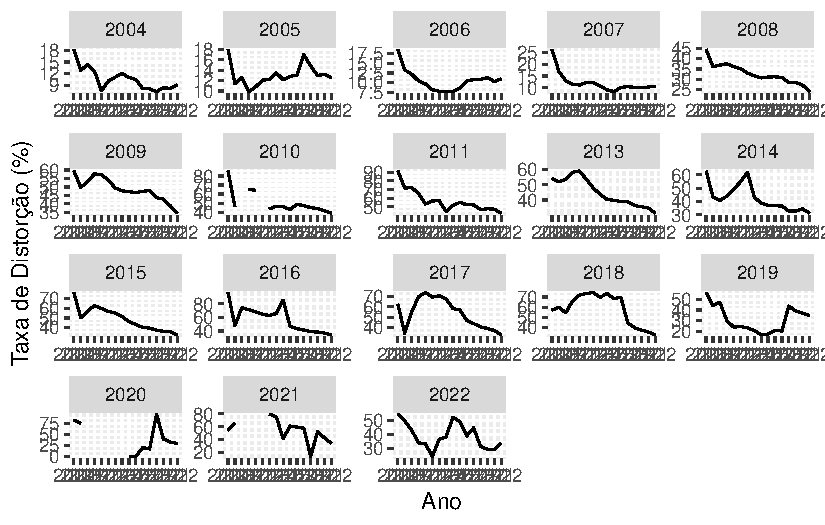
\includegraphics{script_files/figure-latex/unnamed-chunk-12-4.pdf}

\begin{Shaded}
\begin{Highlighting}[]
\FunctionTok{datasummary\_balance}\NormalTok{(}\SpecialCharTok{\textasciitilde{}}\NormalTok{tratado, dados\_ice\_v3 }\SpecialCharTok{\%\textgreater{}\%} 
                      \FunctionTok{select}\NormalTok{(tratado, e\_mora\_mais\_de\_6\_pessoas}\SpecialCharTok{:}\NormalTok{e\_trabalhou\_ou\_procurou,}
\NormalTok{                             dependencia\_administrativa}\SpecialCharTok{:}\NormalTok{ativa, predio}\SpecialCharTok{:}\NormalTok{esgoto,}
                             \FunctionTok{starts\_with}\NormalTok{(}\StringTok{\textquotesingle{}p\_\textquotesingle{}}\NormalTok{)),}
                    \AttributeTok{dinm\_statistic =} \StringTok{"p.value"}\NormalTok{)}
\end{Highlighting}
\end{Shaded}

\begin{table}
\centering
\begin{tblr}[         %% tabularray outer open
]                     %% tabularray outer close
{                     %% tabularray inner open
colspec={Q[]Q[]Q[]Q[]Q[]Q[]Q[]Q[]},
cell{1}{3}={c=2,}{halign=c,},
cell{1}{5}={c=2,}{halign=c,},
column{1}={halign=l,},
column{2}={halign=l,},
column{3}={halign=r,},
column{4}={halign=r,},
column{5}={halign=r,},
column{6}={halign=r,},
column{7}={halign=r,},
column{8}={halign=r,},
row{1}={halign=c,},
hline{32}={1,2,3,4,5,6,7,8}{solid, 0.05em, black},
}                     %% tabularray inner close
\toprule
&  & 0 &  & 1 &  &  &  \\ \cmidrule[lr]{3-4}\cmidrule[lr]{5-6}
&    & Mean & Std. Dev. & Mean & Std. Dev. & Diff. in Means & p \\ \midrule %% TinyTableHeader
e\_mora\_mais\_de\_6\_pessoas      &   & \num{0.0}   & \num{0.1}  & \num{0.1}  & \num{0.1}  & \num{0.0}  & <0.001 \\
e\_renda\_familia\_5\_salarios      &   & \num{0.2}   & \num{0.3}  & \num{0.0}  & \num{0.1}  & \num{-0.1} & <0.001 \\
e\_trabalhou\_ou\_procurou           &   & \num{0.4}   & \num{0.3}  & \num{0.4}  & \num{0.3}  & \num{-0.1} & <0.001 \\
n\_mulheres\_em\_1                   &   & \num{52.0}  & \num{62.8} & \num{83.4} & \num{63.9} & \num{31.4} & <0.001 \\
n\_mulheres\_em\_2                   &   & \num{44.2}  & \num{52.2} & \num{64.0} & \num{47.7} & \num{19.8} & <0.001 \\
n\_mulheres\_em\_3                   &   & \num{39.0}  & \num{46.1} & \num{61.9} & \num{51.0} & \num{22.9} & <0.001 \\
rural                                   &   & \num{0.0}   & \num{0.2}  & \num{0.0}  & \num{0.1}  & \num{0.0}  & <0.001 \\
ativa                                   &   & \num{1.0}   & \num{0.0}  & \num{1.0}  & \num{0.0}  & \num{0.0}  &        \\
predio                                  &   & \num{1.0}   & \num{0.1}  & \num{1.0}  & \num{0.0}  & \num{0.0}  & <0.001 \\
diretoria                               &   & \num{0.9}   & \num{0.2}  & \num{1.0}  & \num{0.2}  & \num{0.0}  & <0.001 \\
biblioteca                              &   & \num{0.6}   & \num{0.5}  & \num{0.7}  & \num{0.5}  & \num{0.1}  & <0.001 \\
sala\_leitura                          &   & \num{0.5}   & \num{0.5}  & \num{0.4}  & \num{0.5}  & \num{-0.1} & <0.001 \\
lab\_info                              &   & \num{0.9}   & \num{0.3}  & \num{1.0}  & \num{0.2}  & \num{0.1}  & <0.001 \\
lab\_ciencias                          &   & \num{0.4}   & \num{0.5}  & \num{0.6}  & \num{0.5}  & \num{0.2}  & <0.001 \\
quadra\_esportes                       &   & \num{0.8}   & \num{0.4}  & \num{0.8}  & \num{0.4}  & \num{0.0}  & 0.005  \\
internet                                &   & \num{1.0}   & \num{0.2}  & \num{1.0}  & \num{0.1}  & \num{0.0}  & <0.001 \\
lixo\_coleta                           &   & \num{1.0}   & \num{0.1}  & \num{1.0}  & \num{0.1}  & \num{0.0}  & <0.001 \\
eletricidade                            &   & \num{1.0}   & \num{0.0}  & \num{1.0}  & \num{0.0}  & \num{0.0}  & 0.687  \\
agua                                    &   & \num{1.0}   & \num{0.2}  & \num{1.0}  & \num{0.1}  & \num{0.0}  & <0.001 \\
esgoto                                  &   & \num{0.8}   & \num{0.4}  & \num{0.7}  & \num{0.4}  & \num{-0.1} & <0.001 \\
p\_mulheres\_em\_1                   &   & \num{0.5}   & \num{0.1}  & \num{0.5}  & \num{0.1}  & \num{0.0}  & <0.001 \\
p\_mulheres\_em\_2                   &   & \num{0.5}   & \num{0.1}  & \num{0.6}  & \num{0.1}  & \num{0.0}  & <0.001 \\
p\_mulheres\_em\_3                   &   & \num{0.5}   & \num{0.1}  & \num{0.6}  & \num{0.1}  & \num{0.0}  & <0.001 \\
p\_brancos\_em\_1                    &   & \num{0.6}   & \num{0.3}  & \num{0.4}  & \num{0.2}  & \num{-0.2} & <0.001 \\
p\_brancos\_em\_2                    &   & \num{0.6}   & \num{0.3}  & \num{0.4}  & \num{0.2}  & \num{-0.2} & <0.001 \\
p\_brancos\_em\_3                    &   & \num{0.6}   & \num{0.3}  & \num{0.4}  & \num{0.2}  & \num{-0.2} & <0.001 \\
p\_alu\_transporte\_publico\_em\_1 &   & \num{0.2}   & \num{0.3}  & \num{0.2}  & \num{0.3}  & \num{0.0}  & <0.001 \\
p\_alu\_transporte\_publico\_em\_2 &   & \num{0.2}   & \num{0.3}  & \num{0.2}  & \num{0.3}  & \num{0.0}  & <0.001 \\
p\_alu\_transporte\_publico\_em\_3 &   & \num{0.2}   & \num{0.3}  & \num{0.2}  & \num{0.3}  & \num{0.0}  & <0.001 \\
&   & N            & Pct.        & N           & Pct.        &             &        \\
dependencia\_administrativa            & 1 & \num{637}   & \num{0.7}  & \num{0}    & \num{0.0}  &             &        \\
& 2 & \num{50298} & \num{57.4} & \num{3923} & \num{98.7} &             &        \\
& 3 & \num{5568}  & \num{6.4}  & \num{51}   & \num{1.3}  &             &        \\
& 4 & \num{31155} & \num{35.5} & \num{0}    & \num{0.0}  &             &        \\
\bottomrule
\end{tblr}
\end{table}

\begin{Shaded}
\begin{Highlighting}[]
\FunctionTok{datasummary\_skim}\NormalTok{(dados\_ice\_v3 }\SpecialCharTok{\%\textgreater{}\%} 
                      \FunctionTok{select}\NormalTok{(tratado, e\_mora\_mais\_de\_6\_pessoas}\SpecialCharTok{:}\NormalTok{e\_trabalhou\_ou\_procurou,}
\NormalTok{                             dependencia\_administrativa}\SpecialCharTok{:}\NormalTok{ativa, predio}\SpecialCharTok{:}\NormalTok{esgoto,}
                             \FunctionTok{starts\_with}\NormalTok{(}\StringTok{\textquotesingle{}p\_\textquotesingle{}}\NormalTok{)),}
                 \AttributeTok{fun\_numeric =} \FunctionTok{list}\NormalTok{(}\AttributeTok{Mean =}\NormalTok{ Mean, }\AttributeTok{SD =}\NormalTok{ SD))}
\end{Highlighting}
\end{Shaded}

\begin{table}
\centering
\begin{tblr}[         %% tabularray outer open
]                     %% tabularray outer close
{                     %% tabularray inner open
colspec={Q[]Q[]Q[]},
hline{32}={1,2,3}{solid, 0.1em, black},
}                     %% tabularray inner close
\toprule
& Mean & SD \\ \midrule %% TinyTableHeader
tratado & 0.0 & 0.2 \\
(mean) e\_mora\_mais\_de\_6\_pessoas & 0.0 & 0.1 \\
(mean) e\_renda\_familia\_5\_salarios & 0.2 & 0.3 \\
(mean) e\_trabalhou\_ou\_procurou & 0.4 & 0.3 \\
n\_mulheres\_em\_1 & 53.4 & 63.2 \\
n\_mulheres\_em\_2 & 45.0 & 52.2 \\
n\_mulheres\_em\_3 & 40.0 & 46.5 \\
rural & 0.0 & 0.2 \\
ativa & 1.0 & 0.0 \\
predio & 1.0 & 0.1 \\
diretoria & 0.9 & 0.2 \\
biblioteca & 0.6 & 0.5 \\
sala\_leitura & 0.5 & 0.5 \\
lab\_info & 0.9 & 0.3 \\
lab\_ciencias & 0.5 & 0.5 \\
quadra\_esportes & 0.8 & 0.4 \\
internet & 1.0 & 0.2 \\
lixo\_coleta & 1.0 & 0.1 \\
eletricidade & 1.0 & 0.0 \\
agua & 1.0 & 0.2 \\
esgoto & 0.8 & 0.4 \\
p\_mulheres\_em\_1 & 0.5 & 0.1 \\
p\_mulheres\_em\_2 & 0.5 & 0.1 \\
p\_mulheres\_em\_3 & 0.5 & 0.1 \\
p\_brancos\_em\_1 & 0.6 & 0.3 \\
p\_brancos\_em\_2 & 0.6 & 0.3 \\
p\_brancos\_em\_3 & 0.6 & 0.3 \\
(mean) p\_alu\_transporte\_publico\_em\_1 & 0.2 & 0.3 \\
(mean) p\_alu\_transporte\_publico\_em\_2 & 0.2 & 0.3 \\
(mean) p\_alu\_transporte\_publico\_em\_3 & 0.2 & 0.3 \\
dependencia\_administrativa & N & \% \\
1 & 637 & 0.7 \\
2 & 54221 & 59.2 \\
3 & 5619 & 6.1 \\
4 & 31155 & 34.0 \\
\bottomrule
\end{tblr}
\end{table}

\begin{Shaded}
\begin{Highlighting}[]
\FunctionTok{datasummary\_balance}\NormalTok{(}\SpecialCharTok{\textasciitilde{}}\NormalTok{tratado, dados\_ice\_v3 }\SpecialCharTok{\%\textgreater{}\%} 
                      \FunctionTok{select}\NormalTok{(tratado, }\FunctionTok{starts\_with}\NormalTok{(}\StringTok{\textquotesingle{}enem\_\textquotesingle{}}\NormalTok{), }
\NormalTok{                             aba\_em, apr\_em, rep\_em, dist\_em),}
                    \AttributeTok{dinm\_statistic =} \StringTok{"p.value"}\NormalTok{)}
\end{Highlighting}
\end{Shaded}

\begin{table}
\centering
\begin{tblr}[         %% tabularray outer open
]                     %% tabularray outer close
{                     %% tabularray inner open
colspec={Q[]Q[]Q[]Q[]Q[]Q[]Q[]},
cell{1}{2}={c=2,}{halign=c,},
cell{1}{4}={c=2,}{halign=c,},
column{1}={halign=l,},
column{2}={halign=r,},
column{3}={halign=r,},
column{4}={halign=r,},
column{5}={halign=r,},
column{6}={halign=r,},
column{7}={halign=r,},
row{1}={halign=c,},
}                     %% tabularray inner close
\toprule
& 0 &  & 1 &  &  &  \\ \cmidrule[lr]{2-3}\cmidrule[lr]{4-5}
& Mean & Std. Dev. & Mean & Std. Dev. & Diff. in Means & p \\ \midrule %% TinyTableHeader
enem\_nota\_redacao    & \num{427.7} & \num{152.7} & \num{412.6} & \num{106.6} & \num{-15.1} & <0.001 \\
enem\_nota\_matematica & \num{502.9} & \num{75.4}  & \num{470.2} & \num{35.5}  & \num{-32.7} & <0.001 \\
enem\_nota\_linguagens & \num{505.8} & \num{50.3}  & \num{483.7} & \num{30.8}  & \num{-22.1} & <0.001 \\
enem\_nota\_humanas    & \num{521.2} & \num{59.3}  & \num{497.2} & \num{43.5}  & \num{-24.0} & <0.001 \\
enem\_nota\_ciencias   & \num{479.9} & \num{54.8}  & \num{454.0} & \num{26.9}  & \num{-25.9} & <0.001 \\
enem\_nota\_objetivab  & \num{502.5} & \num{54.6}  & \num{476.3} & \num{27.6}  & \num{-26.2} & <0.001 \\
aba\_em                 & \num{4.6}   & \num{6.9}   & \num{4.6}   & \num{6.7}   & \num{0.0}   & 0.717  \\
apr\_em                 & \num{85.9}  & \num{12.0}  & \num{87.0}  & \num{10.5}  & \num{1.1}   & <0.001 \\
rep\_em                 & \num{9.5}   & \num{8.5}   & \num{8.3}   & \num{7.2}   & \num{-1.2}  & <0.001 \\
dist\_em                & \num{21.2}  & \num{18.1}  & \num{25.4}  & \num{17.9}  & \num{4.1}   & <0.001 \\
\bottomrule
\end{tblr}
\end{table}

\begin{Shaded}
\begin{Highlighting}[]
\FunctionTok{datasummary\_skim}\NormalTok{(dados\_ice\_v3 }\SpecialCharTok{\%\textgreater{}\%} 
                   \FunctionTok{select}\NormalTok{(tratado, }\FunctionTok{starts\_with}\NormalTok{(}\StringTok{\textquotesingle{}enem\_\textquotesingle{}}\NormalTok{),}
\NormalTok{                          aba\_em, apr\_em, rep\_em, dist\_em),}
                 \AttributeTok{fun\_numeric =} \FunctionTok{list}\NormalTok{(}\AttributeTok{Mean =}\NormalTok{ Mean, }\AttributeTok{SD =}\NormalTok{ SD))}
\end{Highlighting}
\end{Shaded}

\begin{table}
\centering
\begin{tblr}[         %% tabularray outer open
]                     %% tabularray outer close
{                     %% tabularray inner open
colspec={Q[]Q[]Q[]},
column{1}={halign=l,},
column{2}={halign=l,},
column{3}={halign=l,},
}                     %% tabularray inner close
\toprule
& Mean & SD \\ \midrule %% TinyTableHeader
tratado & 0.0 & 0.2 \\
(mean) enem\_nota\_redacao & 427.1 & 151.0 \\
(mean) enem\_nota\_matematica & 501.4 & 74.4 \\
(mean) enem\_nota\_linguagens & 504.9 & 49.8 \\
(mean) enem\_nota\_humanas & 520.1 & 58.9 \\
(mean) enem\_nota\_ciencias & 478.8 & 54.1 \\
enem\_nota\_objetivab & 501.4 & 54.0 \\
aba\_em & 4.6 & 6.9 \\
apr\_em & 85.9 & 11.9 \\
rep\_em & 9.5 & 8.4 \\
dist\_em & 21.5 & 18.1 \\
\bottomrule
\end{tblr}
\end{table}

\begin{Shaded}
\begin{Highlighting}[]
\FunctionTok{datasummary\_balance}\NormalTok{(}\SpecialCharTok{\textasciitilde{}}\NormalTok{tratado, painel\_indicadores\_simplificado }\SpecialCharTok{\%\textgreater{}\%} 
                      \FunctionTok{select}\NormalTok{(tratado, dependencia\_administrativa}\SpecialCharTok{:}\NormalTok{internet),}
                    \AttributeTok{dinm\_statistic =} \StringTok{"p.value"}\NormalTok{)}
\end{Highlighting}
\end{Shaded}

\begin{table}
\centering
\begin{tblr}[         %% tabularray outer open
]                     %% tabularray outer close
{                     %% tabularray inner open
colspec={Q[]Q[]Q[]Q[]Q[]Q[]Q[]Q[]},
cell{1}{3}={c=2,}{halign=c,},
cell{1}{5}={c=2,}{halign=c,},
column{1}={halign=l,},
column{2}={halign=l,},
column{3}={halign=r,},
column{4}={halign=r,},
column{5}={halign=r,},
column{6}={halign=r,},
column{7}={halign=r,},
column{8}={halign=r,},
row{1}={halign=c,},
hline{19}={1,2,3,4,5,6,7,8}{solid, 0.05em, black},
}                     %% tabularray inner close
\toprule
&  & 0 &  & 1 &  &  &  \\ \cmidrule[lr]{3-4}\cmidrule[lr]{5-6}
&    & Mean & Std. Dev. & Mean & Std. Dev. & Diff. in Means & p \\ \midrule %% TinyTableHeader
rural                         &   & \num{0.2}  & \num{0.4}  & \num{0.1}    & \num{0.3}  & \num{-0.1} & <0.001 \\
ativa                         &   & \num{1.0}  & \num{0.0}  & \num{1.0}    & \num{0.0}  & \num{0.0}  &        \\
agua                          &   & \num{0.8}  & \num{0.4}  & \num{0.9}    & \num{0.3}  & \num{0.1}  & <0.001 \\
eletricidade                  &   & \num{1.0}  & \num{0.1}  & \num{1.0}    & \num{0.1}  & \num{0.0}  & 0.105  \\
esgoto                        &   & \num{0.5}  & \num{0.5}  & \num{0.6}    & \num{0.5}  & \num{0.1}  & <0.001 \\
lixo\_coleta                 &   & \num{0.9}  & \num{0.3}  & \num{0.9}    & \num{0.3}  & \num{0.0}  & <0.001 \\
quadra\_esportes             &   & \num{0.5}  & \num{0.5}  & \num{0.5}    & \num{0.5}  & \num{0.0}  & 0.670  \\
lab\_info                    &   & \num{0.8}  & \num{0.4}  & \num{0.9}    & \num{0.4}  & \num{0.0}  & <0.001 \\
lab\_ciencias                &   & \num{0.6}  & \num{0.5}  & \num{0.4}    & \num{0.5}  & \num{-0.1} & <0.001 \\
predio                        &   & \num{1.0}  & \num{0.1}  & \num{1.0}    & \num{0.1}  & \num{0.0}  & 0.006  \\
biblioteca                    &   & \num{0.8}  & \num{0.4}  & \num{0.7}    & \num{0.5}  & \num{-0.2} & <0.001 \\
sala\_leitura                &   & \num{0.4}  & \num{0.5}  & \num{0.3}    & \num{0.5}  & \num{-0.1} & <0.001 \\
diretoria                     &   & \num{0.9}  & \num{0.2}  & \num{0.9}    & \num{0.3}  & \num{0.0}  & <0.001 \\
n\_salas\_exis              &   & \num{19.6} & \num{64.6} & \num{12.5}   & \num{11.9} & \num{-7.0} & <0.001 \\
quantidade\_sala\_utilizada &   & \num{17.9} & \num{26.9} & \num{12.1}   & \num{9.7}  & \num{-5.7} & <0.001 \\
internet                      &   & \num{0.8}  & \num{0.4}  & \num{0.9}    & \num{0.3}  & \num{0.1}  & <0.001 \\
&   & N           & Pct.        & N             & Pct.        &             &        \\
dependencia\_administrativa  & 2 & \num{899}  & \num{0.0}  & \num{300145} & \num{91.0} &             &        \\
& 4 & \num{0}    & \num{0.0}  & \num{0}      & \num{0.0}  &             &        \\
& 1 & \num{6824} & \num{0.3}  & \num{1}      & \num{0.0}  &             &        \\
& 3 & \num{5691} & \num{0.2}  & \num{28}     & \num{0.0}  &             &        \\
\bottomrule
\end{tblr}
\end{table}

\begin{Shaded}
\begin{Highlighting}[]
\FunctionTok{datasummary\_skim}\NormalTok{(painel\_indicadores\_simplificado }\SpecialCharTok{\%\textgreater{}\%}
                   \FunctionTok{select}\NormalTok{(tratado, dependencia\_administrativa}\SpecialCharTok{:}\NormalTok{internet))}
\end{Highlighting}
\end{Shaded}

\begin{table}
\centering
\begin{tblr}[         %% tabularray outer open
]                     %% tabularray outer close
{                     %% tabularray inner open
colspec={Q[]Q[]Q[]Q[]Q[]Q[]Q[]Q[]Q[]},
hline{19}={1,2,3,4,5,6,7,8,9}{solid, 0.1em, black},
}                     %% tabularray inner close
\toprule
& Unique & Missing Pct. & Mean & SD & Min & Median & Max & Histogram \\ \midrule %% TinyTableHeader
tratado & 2 & 0 & 0.1 & 0.3 & 0.0 & 0.0 & 1.0 & 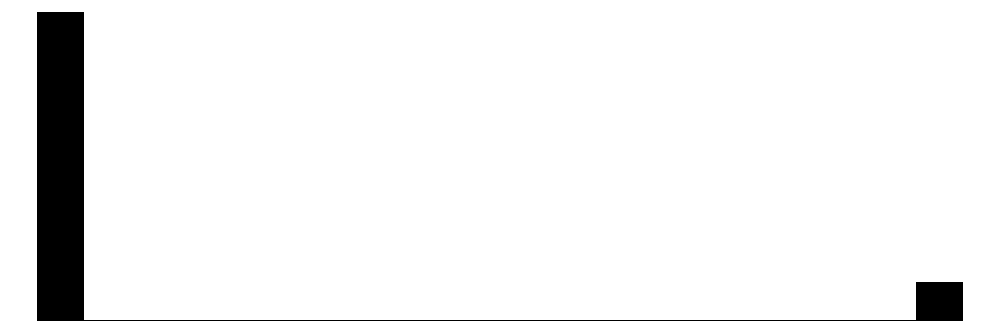
\includegraphics[height=1em]{tinytable_assets/id0k5ig2e1vdtk5n8lt3qn.png} \\
rural & 3 & 90 & 0.1 & 0.3 & 0.0 & 0.0 & 1.0 & 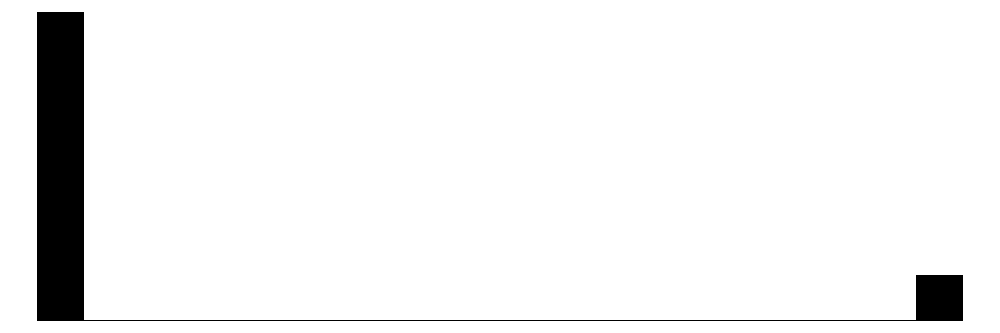
\includegraphics[height=1em]{tinytable_assets/id47m9klz5dikl7tlg0xu5.png} \\
ativa & 2 & 90 & 1.0 & 0.0 & 1.0 & 1.0 & 1.0 & 
\includegraphics[height=1em]{tinytable_assets/idegmvjv3dtq3bcv0iyyj3.png} \\
agua & 3 & 90 & 0.9 & 0.3 & 0.0 & 1.0 & 1.0 & 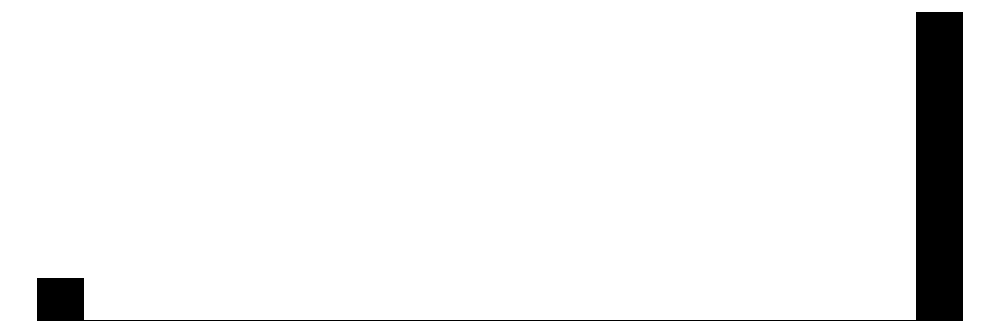
\includegraphics[height=1em]{tinytable_assets/idqpsozryymkpofyoileau.png} \\
eletricidade & 3 & 90 & 1.0 & 0.1 & 0.0 & 1.0 & 1.0 & 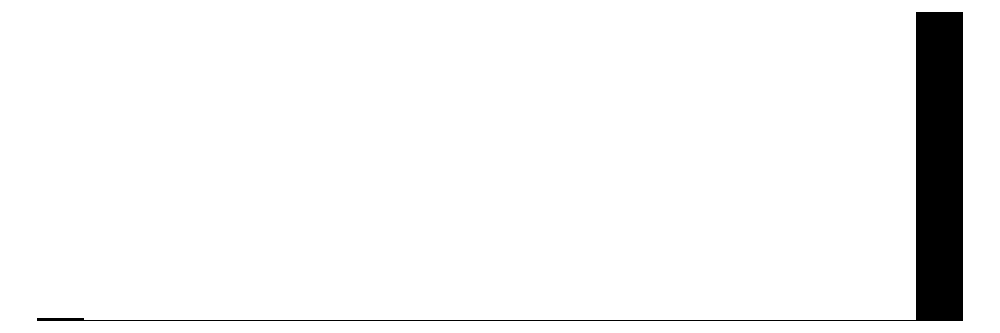
\includegraphics[height=1em]{tinytable_assets/id2x6bk8e4lvidvtsl8lq7.png} \\
esgoto & 3 & 90 & 0.6 & 0.5 & 0.0 & 1.0 & 1.0 & 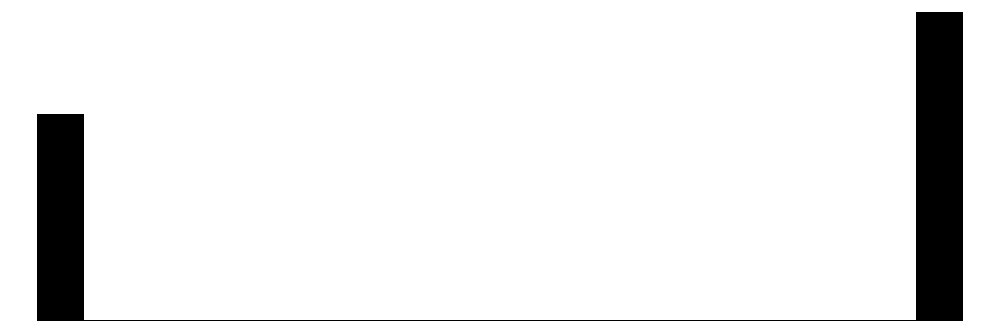
\includegraphics[height=1em]{tinytable_assets/idrhi5sd4etrb3ygfua0fz.png} \\
lixo\_coleta & 3 & 90 & 0.9 & 0.3 & 0.0 & 1.0 & 1.0 & 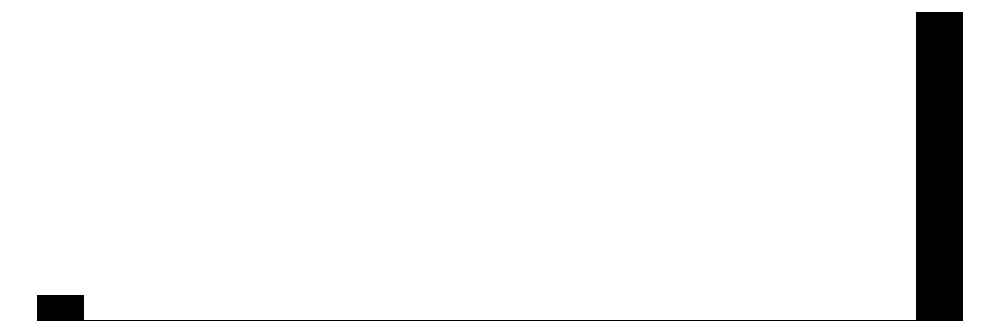
\includegraphics[height=1em]{tinytable_assets/idnhb7epgcxi35e9muftza.png} \\
quadra\_esportes & 3 & 92 & 0.5 & 0.5 & 0.0 & 1.0 & 1.0 & 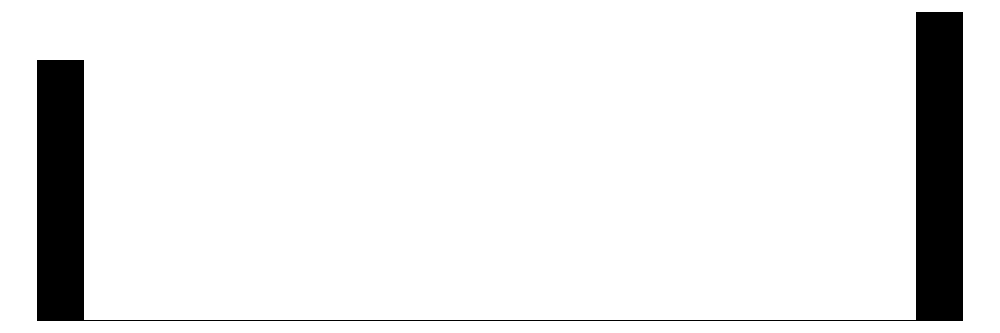
\includegraphics[height=1em]{tinytable_assets/id1z5nrrhwy3zxnduhyhld.png} \\
lab\_info & 3 & 90 & 0.8 & 0.4 & 0.0 & 1.0 & 1.0 & 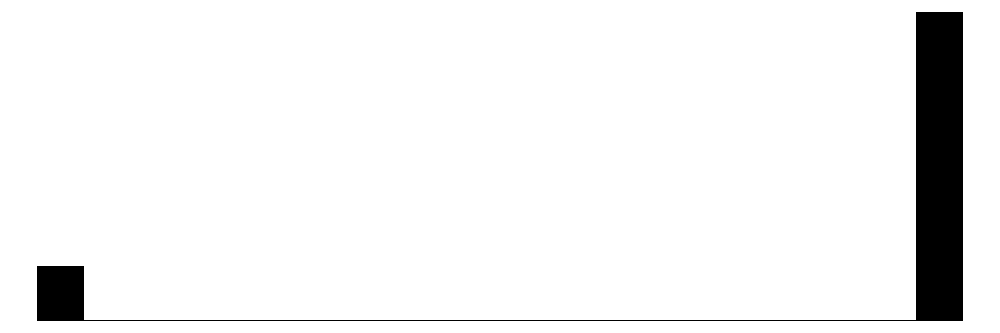
\includegraphics[height=1em]{tinytable_assets/ido39uuvq6699rvi0rzau9.png} \\
lab\_ciencias & 3 & 90 & 0.4 & 0.5 & 0.0 & 0.0 & 1.0 & 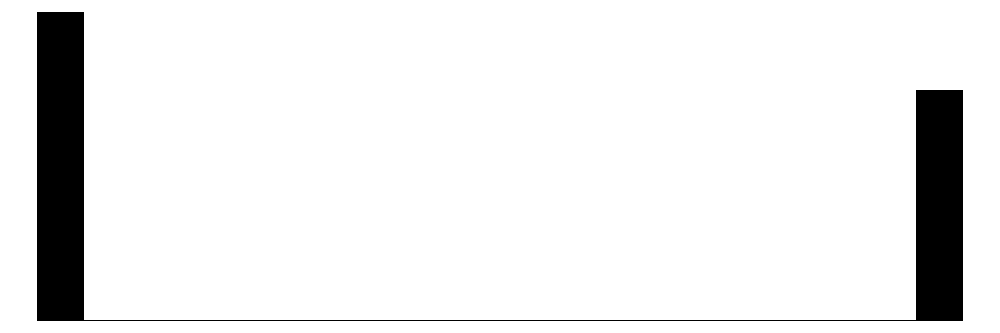
\includegraphics[height=1em]{tinytable_assets/idf58t0k0xd1devc2uwkl6.png} \\
predio & 3 & 90 & 1.0 & 0.1 & 0.0 & 1.0 & 1.0 & 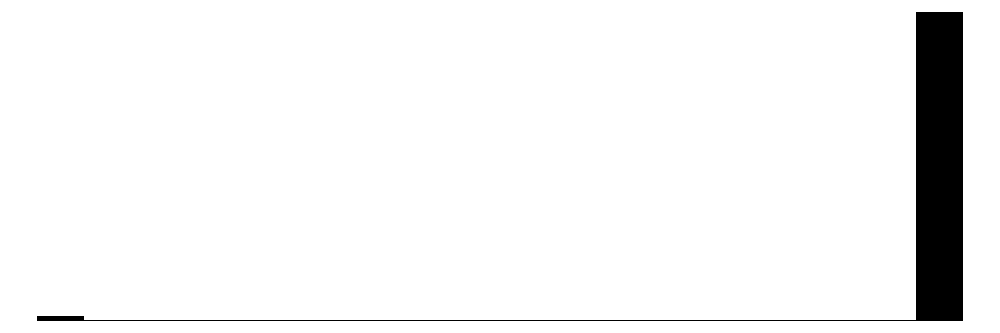
\includegraphics[height=1em]{tinytable_assets/idzais33ro9kcx9wrydxpp.png} \\
biblioteca & 3 & 91 & 0.7 & 0.5 & 0.0 & 1.0 & 1.0 & 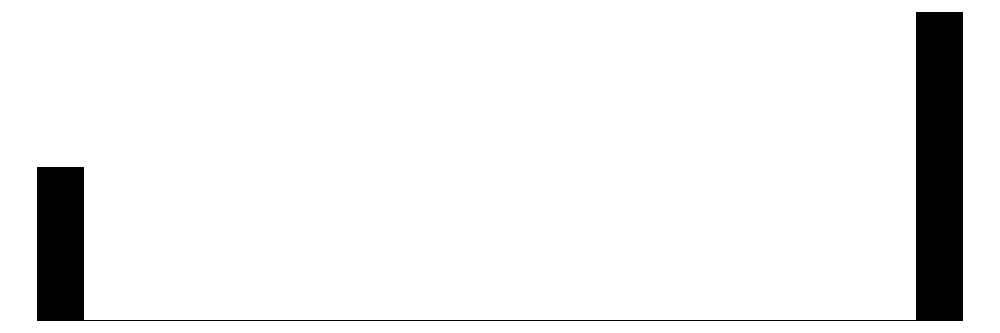
\includegraphics[height=1em]{tinytable_assets/iduy01z9tqfp4xaprseknv.png} \\
sala\_leitura & 3 & 91 & 0.3 & 0.5 & 0.0 & 0.0 & 1.0 & 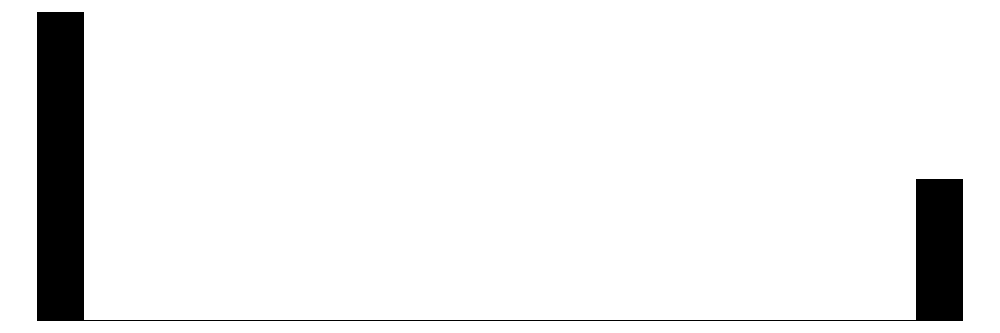
\includegraphics[height=1em]{tinytable_assets/idhzon3pd43zo8jwcuoij5.png} \\
diretoria & 3 & 90 & 0.9 & 0.3 & 0.0 & 1.0 & 1.0 & 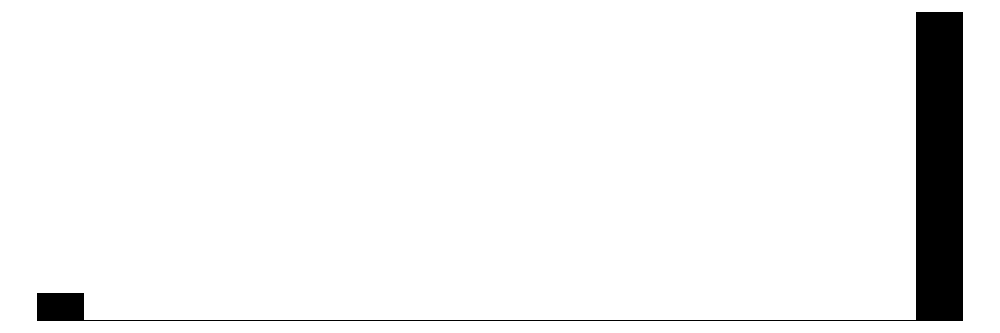
\includegraphics[height=1em]{tinytable_assets/idc9yh80erkavhwe9csc32.png} \\
n\_salas\_exis & 145 & 92 & 12.8 & 17.9 & 0.0 & 12.0 & 2810.0 & 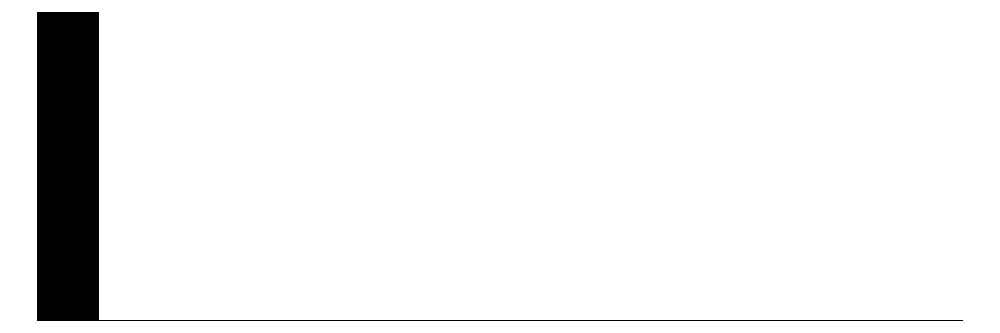
\includegraphics[height=1em]{tinytable_assets/idlkbgu01k6da8anq15rlb.png} \\
quantidade\_sala\_utilizada & 151 & 90 & 12.4 & 11.1 & 1.0 & 11.0 & 2514.0 & 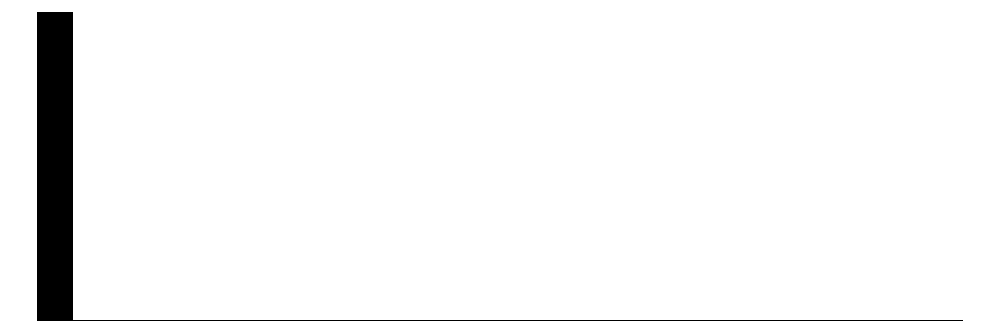
\includegraphics[height=1em]{tinytable_assets/id5ufci37qui3ub6702nr7.png} \\
internet & 3 & 90 & 0.9 & 0.3 & 0.0 & 1.0 & 1.0 & 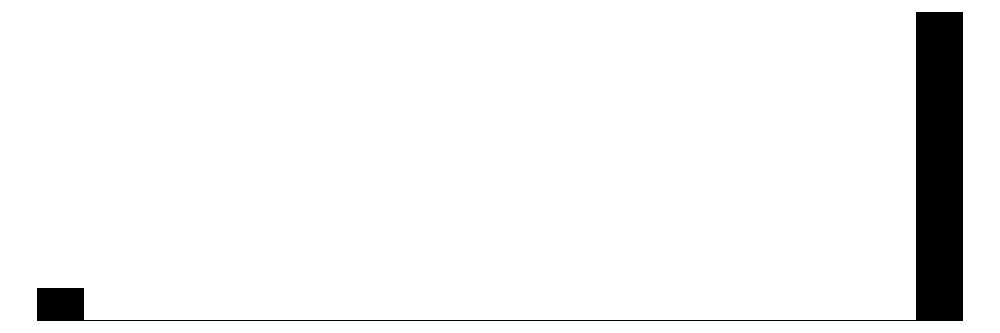
\includegraphics[height=1em]{tinytable_assets/id03v9p343nrfuzw82261r.png} \\
dependencia\_administrativa & N & \% &  &  &  &  &  &  \\
2 & 301044 & 10.1 &  &  &  &  &  &  \\
4 & 0 & 0.0 &  &  &  &  &  &  \\
1 & 6825 & 0.2 &  &  &  &  &  &  \\
3 & 5719 & 0.2 &  &  &  &  &  &  \\
\bottomrule
\end{tblr}
\end{table}

\begin{Shaded}
\begin{Highlighting}[]
\FunctionTok{datasummary\_balance}\NormalTok{(}\SpecialCharTok{\textasciitilde{}}\NormalTok{tratado, painel\_indicadores\_simplificado }\SpecialCharTok{\%\textgreater{}\%} 
                      \FunctionTok{select}\NormalTok{(tratado, }\FunctionTok{ends\_with}\NormalTok{(}\StringTok{\textquotesingle{}em\textquotesingle{}}\NormalTok{)),}
                    \AttributeTok{dinm\_statistic =} \StringTok{"p.value"}\NormalTok{)}
\end{Highlighting}
\end{Shaded}

\begin{table}
\centering
\begin{tblr}[         %% tabularray outer open
]                     %% tabularray outer close
{                     %% tabularray inner open
colspec={Q[]Q[]Q[]Q[]Q[]Q[]Q[]},
cell{1}{2}={c=2,}{halign=c,},
cell{1}{4}={c=2,}{halign=c,},
column{1}={halign=l,},
column{2}={halign=r,},
column{3}={halign=r,},
column{4}={halign=r,},
column{5}={halign=r,},
column{6}={halign=r,},
column{7}={halign=r,},
row{1}={halign=c,},
}                     %% tabularray inner close
\toprule
& 0 &  & 1 &  &  &  \\ \cmidrule[lr]{2-3}\cmidrule[lr]{4-5}
& Mean & Std. Dev. & Mean & Std. Dev. & Diff. in Means & p \\ \midrule %% TinyTableHeader
apr\_em  & \num{93.8} & \num{8.6}  & \num{81.5} & \num{13.2} & \num{-12.3} & <0.001 \\
dist\_em & \num{11.2} & \num{14.2} & \num{33.1} & \num{19.4} & \num{21.9}  & <0.001 \\
rep\_em  & \num{5.0}  & \num{6.7}  & \num{10.0} & \num{9.2}  & \num{5.1}   & <0.001 \\
aba\_em  & \num{1.2}  & \num{5.0}  & \num{8.5}  & \num{9.1}  & \num{7.3}   & <0.001 \\
\bottomrule
\end{tblr}
\end{table}

\begin{Shaded}
\begin{Highlighting}[]
\FunctionTok{datasummary\_skim}\NormalTok{(painel\_indicadores\_simplificado }\SpecialCharTok{\%\textgreater{}\%} 
                      \FunctionTok{select}\NormalTok{(tratado, }\FunctionTok{ends\_with}\NormalTok{(}\StringTok{\textquotesingle{}em\textquotesingle{}}\NormalTok{)))}
\end{Highlighting}
\end{Shaded}

\begin{table}
\centering
\begin{tblr}[         %% tabularray outer open
]                     %% tabularray outer close
{                     %% tabularray inner open
colspec={Q[]Q[]Q[]Q[]Q[]Q[]Q[]Q[]Q[]},
column{1}={halign=l,},
column{2}={halign=l,},
column{3}={halign=l,},
column{4}={halign=l,},
column{5}={halign=l,},
column{6}={halign=l,},
column{7}={halign=l,},
column{8}={halign=l,},
column{9}={halign=l,},
}                     %% tabularray inner close
\toprule
& Unique & Missing Pct. & Mean & SD & Min & Median & Max & Histogram \\ \midrule %% TinyTableHeader
tratado & 2 & 0 & 0.1 & 0.3 & 0.0 & 0.0 & 1.0 & 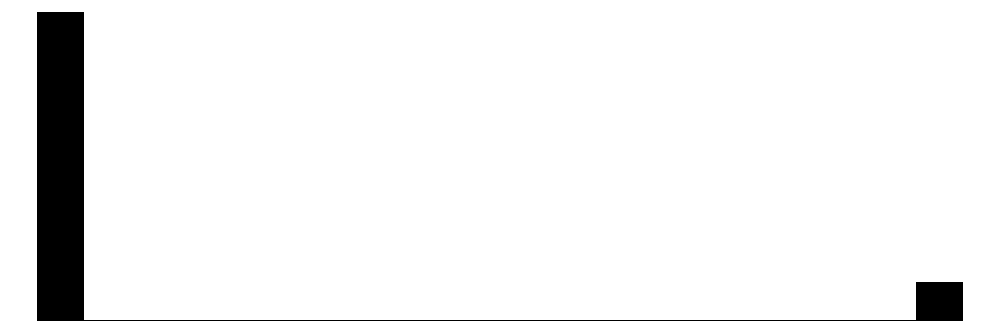
\includegraphics[height=1em]{tinytable_assets/idx2rwm9zpe5mizwmt76a7.png} \\
apr\_em & 820 & 86 & 85.3 & 13.3 & 0.0 & 88.5 & 100.0 & 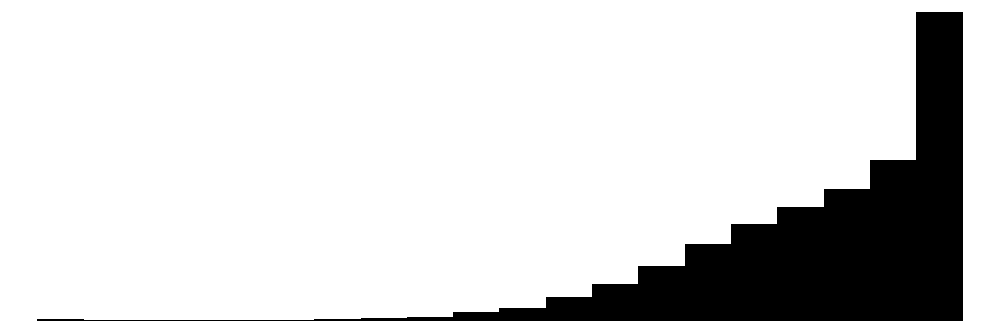
\includegraphics[height=1em]{tinytable_assets/id6ytogniz44ccieis657f.png} \\
dist\_em & 999 & 86 & 26.3 & 20.6 & 0.0 & 21.7 & 100.0 & 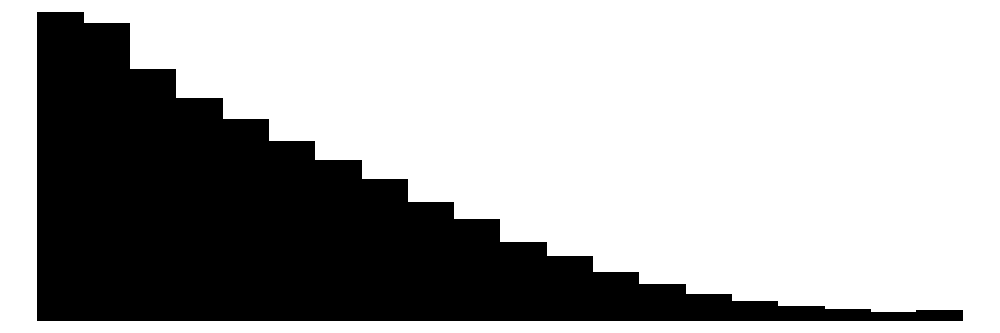
\includegraphics[height=1em]{tinytable_assets/idjyudkk739xkx1t7r6a9p.png} \\
rep\_em & 709 & 86 & 8.5 & 8.8 & 0.0 & 6.1 & 100.0 & 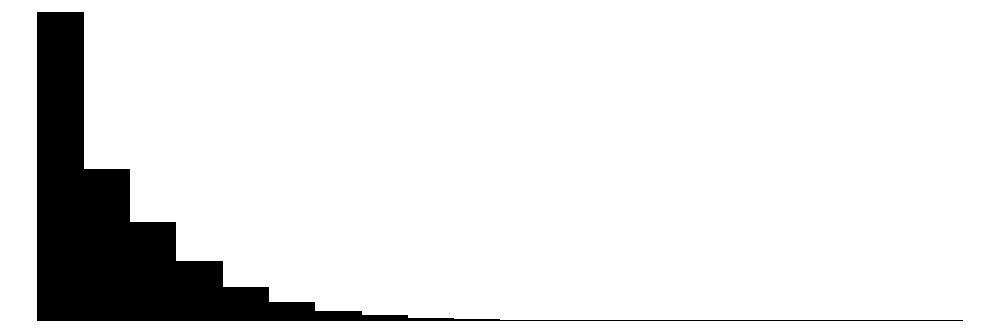
\includegraphics[height=1em]{tinytable_assets/idgxj3tm7ipif8boxi001y.png} \\
aba\_em & 714 & 86 & 6.2 & 8.7 & 0.0 & 2.4 & 100.0 & 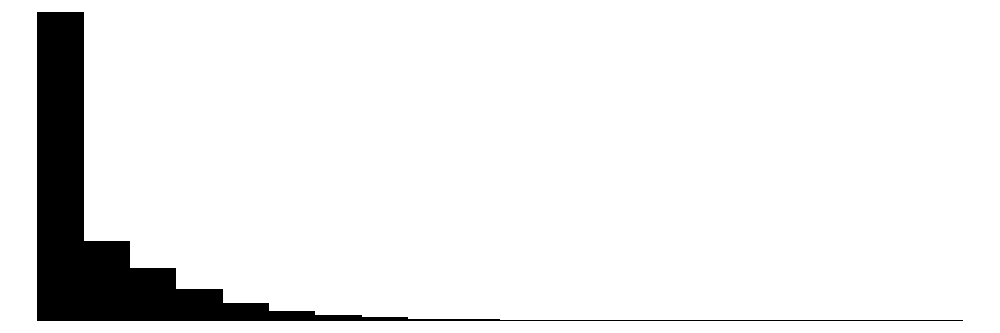
\includegraphics[height=1em]{tinytable_assets/idt1x2xvj9yexh7e4nw5ja.png} \\
\bottomrule
\end{tblr}
\end{table}

\section{Inference}\label{inference}

\subsection{TWFE}\label{twfe}

\subsection{Bacon decomposition}\label{bacon-decomposition}

\subsection{Creating normalized
effects}\label{creating-normalized-effects}

\begin{Shaded}
\begin{Highlighting}[]
\NormalTok{did\_redacao\_norm }\OtherTok{\textless{}{-}}\NormalTok{ did}\SpecialCharTok{::}\FunctionTok{att\_gt}\NormalTok{(}
  \AttributeTok{yname =} \StringTok{"enem\_nota\_redacao"}\NormalTok{,}
  \AttributeTok{tname =} \StringTok{"ano"}\NormalTok{,}
  \AttributeTok{idname =} \StringTok{"codigo\_escola"}\NormalTok{,}
  \AttributeTok{gname =} \StringTok{"ano\_ice"}\NormalTok{, }
  \AttributeTok{data =}\NormalTok{ dados\_ice\_v3\_norm}
\NormalTok{)}

\NormalTok{did\_matematica\_norm }\OtherTok{\textless{}{-}}\NormalTok{ did}\SpecialCharTok{::}\FunctionTok{att\_gt}\NormalTok{(}
  \AttributeTok{yname =} \StringTok{"enem\_nota\_matematica"}\NormalTok{,}
  \AttributeTok{tname =} \StringTok{"ano"}\NormalTok{,}
  \AttributeTok{idname =} \StringTok{"codigo\_escola"}\NormalTok{,}
  \AttributeTok{gname =} \StringTok{"ano\_ice"}\NormalTok{,}
  \AttributeTok{data =}\NormalTok{ dados\_ice\_v3\_norm}
\NormalTok{)}

\NormalTok{did\_linguagem\_norm }\OtherTok{\textless{}{-}}\NormalTok{ did}\SpecialCharTok{::}\FunctionTok{att\_gt}\NormalTok{(}
  \AttributeTok{yname =} \StringTok{"enem\_nota\_linguagens"}\NormalTok{,}
  \AttributeTok{tname =} \StringTok{"ano"}\NormalTok{,}
  \AttributeTok{idname =} \StringTok{"codigo\_escola"}\NormalTok{,}
  \AttributeTok{gname =} \StringTok{"ano\_ice"}\NormalTok{,}
  \AttributeTok{data =}\NormalTok{ dados\_ice\_v3\_norm}
\NormalTok{)}

\NormalTok{did\_ciencias\_norm }\OtherTok{\textless{}{-}}\NormalTok{ did}\SpecialCharTok{::}\FunctionTok{att\_gt}\NormalTok{(}
  \AttributeTok{yname =} \StringTok{"enem\_nota\_ciencias"}\NormalTok{,}
  \AttributeTok{tname =} \StringTok{"ano"}\NormalTok{,}
  \AttributeTok{idname =} \StringTok{"codigo\_escola"}\NormalTok{,}
  \AttributeTok{gname =} \StringTok{"ano\_ice"}\NormalTok{,}
  \AttributeTok{data =}\NormalTok{ dados\_ice\_v3\_norm}
\NormalTok{)}

\NormalTok{did\_humanas\_norm }\OtherTok{\textless{}{-}}\NormalTok{ did}\SpecialCharTok{::}\FunctionTok{att\_gt}\NormalTok{(}
  \AttributeTok{yname =} \StringTok{"enem\_nota\_humanas"}\NormalTok{,}
  \AttributeTok{tname =} \StringTok{"ano"}\NormalTok{,}
  \AttributeTok{idname =} \StringTok{"codigo\_escola"}\NormalTok{,}
  \AttributeTok{gname =} \StringTok{"ano\_ice"}\NormalTok{,}
  \AttributeTok{data =}\NormalTok{ dados\_ice\_v3\_norm}
\NormalTok{)}

\NormalTok{did\_objetiva\_norm }\OtherTok{\textless{}{-}}\NormalTok{ did}\SpecialCharTok{::}\FunctionTok{att\_gt}\NormalTok{(}
  \AttributeTok{yname =} \StringTok{"enem\_nota\_objetivab"}\NormalTok{,}
  \AttributeTok{tname =} \StringTok{"ano"}\NormalTok{,}
  \AttributeTok{idname =} \StringTok{"codigo\_escola"}\NormalTok{,}
  \AttributeTok{gname =} \StringTok{"ano\_ice"}\NormalTok{,}
  \AttributeTok{data =}\NormalTok{ dados\_ice\_v3\_norm}
\NormalTok{)}
\end{Highlighting}
\end{Shaded}

\begin{Shaded}
\begin{Highlighting}[]
\NormalTok{did\_abandono\_norm }\OtherTok{\textless{}{-}}\NormalTok{ did}\SpecialCharTok{::}\FunctionTok{att\_gt}\NormalTok{(}
  \AttributeTok{yname =} \StringTok{"aba\_em"}\NormalTok{,}
  \AttributeTok{tname =} \StringTok{"ano"}\NormalTok{,}
  \AttributeTok{idname =} \StringTok{"codigo\_escola"}\NormalTok{,}
  \AttributeTok{gname =} \StringTok{"ano\_ice"}\NormalTok{,}
  \AttributeTok{data =}\NormalTok{ painel\_indicadores\_simplificado\_norm}
\NormalTok{)}

\NormalTok{did\_reprovacao\_norm }\OtherTok{\textless{}{-}}\NormalTok{ did}\SpecialCharTok{::}\FunctionTok{att\_gt}\NormalTok{(}
  \AttributeTok{yname =} \StringTok{"rep\_em"}\NormalTok{,}
  \AttributeTok{tname =} \StringTok{"ano"}\NormalTok{,}
  \AttributeTok{idname =} \StringTok{"codigo\_escola"}\NormalTok{,}
  \AttributeTok{gname =} \StringTok{"ano\_ice"}\NormalTok{,}
  \AttributeTok{data =}\NormalTok{ painel\_indicadores\_simplificado\_norm}
\NormalTok{)}

\NormalTok{did\_aprovacao\_norm }\OtherTok{\textless{}{-}}\NormalTok{ did}\SpecialCharTok{::}\FunctionTok{att\_gt}\NormalTok{(}
  \AttributeTok{yname =} \StringTok{"apr\_em"}\NormalTok{,}
  \AttributeTok{tname =} \StringTok{"ano"}\NormalTok{,}
  \AttributeTok{idname =} \StringTok{"codigo\_escola"}\NormalTok{,}
  \AttributeTok{gname =} \StringTok{"ano\_ice"}\NormalTok{,}
  \AttributeTok{data =}\NormalTok{ painel\_indicadores\_simplificado\_norm}
\NormalTok{)}

\NormalTok{did\_distorcao\_norm }\OtherTok{\textless{}{-}}\NormalTok{ did}\SpecialCharTok{::}\FunctionTok{att\_gt}\NormalTok{(}
  \AttributeTok{yname =} \StringTok{"dist\_em"}\NormalTok{,}
  \AttributeTok{tname =} \StringTok{"ano"}\NormalTok{,}
  \AttributeTok{idname =} \StringTok{"codigo\_escola"}\NormalTok{,}
  \AttributeTok{gname =} \StringTok{"ano\_ice"}\NormalTok{,}
  \AttributeTok{data =}\NormalTok{ painel\_indicadores\_simplificado\_norm}
\NormalTok{)}
\end{Highlighting}
\end{Shaded}

\subsubsection{Dynamic results}\label{dynamic-results}

\begin{Shaded}
\begin{Highlighting}[]
\FunctionTok{aggte}\NormalTok{(did\_redacao\_norm, }\AttributeTok{type =} \StringTok{"dynamic"}\NormalTok{, }\AttributeTok{na.rm =}\NormalTok{ T)}
\end{Highlighting}
\end{Shaded}

\begin{verbatim}

Call:
aggte(MP = did_redacao_norm, type = "dynamic", na.rm = T)

Reference: Callaway, Brantly and Pedro H.C. Sant'Anna.  "Difference-in-Differences with Multiple Time Periods." Journal of Econometrics, Vol. 225, No. 2, pp. 200-230, 2021. <https://doi.org/10.1016/j.jeconom.2020.12.001>, <https://arxiv.org/abs/1803.09015> 


Overall summary of ATT's based on event-study/dynamic aggregation:  
   ATT    Std. Error     [ 95%  Conf. Int.]  
 0.169        0.0303     0.1096      0.2284 *


Dynamic Effects:
 Event time Estimate Std. Error [95% Simult.  Conf. Band]  
         -5   0.0216     0.1100       -0.2742      0.3174  
         -4  -0.0095     0.0539       -0.1544      0.1354  
         -3  -0.0442     0.0389       -0.1488      0.0604  
         -2   0.0075     0.0301       -0.0734      0.0884  
         -1  -0.0984     0.0246       -0.1646     -0.0321 *
          0  -0.0137     0.0311       -0.0972      0.0698  
          1   0.0110     0.0313       -0.0732      0.0952  
          2   0.1594     0.0303        0.0780      0.2407 *
          3   0.3306     0.0395        0.2245      0.4367 *
          4   0.2096     0.0587        0.0518      0.3675 *
          5   0.3170     0.0687        0.1322      0.5019 *
---
Signif. codes: `*' confidence band does not cover 0

Control Group:  Never Treated,  Anticipation Periods:  0
Estimation Method:  Doubly Robust
\end{verbatim}

\begin{Shaded}
\begin{Highlighting}[]
\FunctionTok{aggte}\NormalTok{(did\_matematica\_norm, }\AttributeTok{type =} \StringTok{"dynamic"}\NormalTok{, }\AttributeTok{na.rm =}\NormalTok{ T)}
\end{Highlighting}
\end{Shaded}

\begin{verbatim}

Call:
aggte(MP = did_matematica_norm, type = "dynamic", na.rm = T)

Reference: Callaway, Brantly and Pedro H.C. Sant'Anna.  "Difference-in-Differences with Multiple Time Periods." Journal of Econometrics, Vol. 225, No. 2, pp. 200-230, 2021. <https://doi.org/10.1016/j.jeconom.2020.12.001>, <https://arxiv.org/abs/1803.09015> 


Overall summary of ATT's based on event-study/dynamic aggregation:  
    ATT    Std. Error     [ 95%  Conf. Int.]  
 0.1524        0.0236     0.1061      0.1987 *


Dynamic Effects:
 Event time Estimate Std. Error [95% Simult.  Conf. Band]  
         -5  -0.0772     0.0751       -0.2784      0.1240  
         -4  -0.0957     0.0370       -0.1947      0.0034  
         -3  -0.1010     0.0258       -0.1701     -0.0319 *
         -2  -0.0737     0.0201       -0.1274     -0.0200 *
         -1   0.0163     0.0178       -0.0313      0.0640  
          0  -0.0318     0.0201       -0.0857      0.0221  
          1   0.0684     0.0231        0.0066      0.1302 *
          2   0.2462     0.0242        0.1815      0.3110 *
          3   0.3078     0.0340        0.2168      0.3988 *
          4   0.1533     0.0450        0.0327      0.2738 *
          5   0.1705     0.0464        0.0463      0.2948 *
---
Signif. codes: `*' confidence band does not cover 0

Control Group:  Never Treated,  Anticipation Periods:  0
Estimation Method:  Doubly Robust
\end{verbatim}

\begin{Shaded}
\begin{Highlighting}[]
\FunctionTok{aggte}\NormalTok{(did\_linguagem\_norm, }\AttributeTok{type =} \StringTok{"dynamic"}\NormalTok{, }\AttributeTok{na.rm =}\NormalTok{ T)}
\end{Highlighting}
\end{Shaded}

\begin{verbatim}

Call:
aggte(MP = did_linguagem_norm, type = "dynamic", na.rm = T)

Reference: Callaway, Brantly and Pedro H.C. Sant'Anna.  "Difference-in-Differences with Multiple Time Periods." Journal of Econometrics, Vol. 225, No. 2, pp. 200-230, 2021. <https://doi.org/10.1016/j.jeconom.2020.12.001>, <https://arxiv.org/abs/1803.09015> 


Overall summary of ATT's based on event-study/dynamic aggregation:  
    ATT    Std. Error     [ 95%  Conf. Int.]  
 0.3322        0.0297     0.2739      0.3904 *


Dynamic Effects:
 Event time Estimate Std. Error [95% Simult.  Conf. Band]  
         -5   0.2320     0.0951       -0.0271      0.4912  
         -4  -0.0179     0.0524       -0.1606      0.1248  
         -3   0.0710     0.0267       -0.0018      0.1437  
         -2   0.0099     0.0216       -0.0488      0.0686  
         -1   0.0226     0.0217       -0.0364      0.0816  
          0   0.0819     0.0222        0.0214      0.1424 *
          1   0.1169     0.0224        0.0558      0.1779 *
          2   0.3079     0.0267        0.2353      0.3805 *
          3   0.3855     0.0412        0.2733      0.4977 *
          4   0.5579     0.0589        0.3974      0.7184 *
          5   0.5429     0.0611        0.3765      0.7093 *
---
Signif. codes: `*' confidence band does not cover 0

Control Group:  Never Treated,  Anticipation Periods:  0
Estimation Method:  Doubly Robust
\end{verbatim}

\begin{Shaded}
\begin{Highlighting}[]
\FunctionTok{aggte}\NormalTok{(did\_ciencias\_norm, }\AttributeTok{type =} \StringTok{"dynamic"}\NormalTok{, }\AttributeTok{na.rm =}\NormalTok{ T)}
\end{Highlighting}
\end{Shaded}

\begin{verbatim}

Call:
aggte(MP = did_ciencias_norm, type = "dynamic", na.rm = T)

Reference: Callaway, Brantly and Pedro H.C. Sant'Anna.  "Difference-in-Differences with Multiple Time Periods." Journal of Econometrics, Vol. 225, No. 2, pp. 200-230, 2021. <https://doi.org/10.1016/j.jeconom.2020.12.001>, <https://arxiv.org/abs/1803.09015> 


Overall summary of ATT's based on event-study/dynamic aggregation:  
    ATT    Std. Error     [ 95%  Conf. Int.]  
 0.3251         0.027     0.2722      0.3781 *


Dynamic Effects:
 Event time Estimate Std. Error [95% Simult.  Conf. Band]  
         -5   0.1330     0.0868       -0.1108      0.3768  
         -4   0.0940     0.0448       -0.0318      0.2198  
         -3   0.0226     0.0280       -0.0562      0.1013  
         -2   0.0016     0.0209       -0.0571      0.0604  
         -1   0.0468     0.0185       -0.0052      0.0987  
          0   0.0805     0.0204        0.0234      0.1377 *
          1   0.1140     0.0214        0.0540      0.1740 *
          2   0.3238     0.0251        0.2535      0.3942 *
          3   0.4027     0.0300        0.3186      0.4869 *
          4   0.4929     0.0530        0.3441      0.6417 *
          5   0.5368     0.0562        0.3788      0.6947 *
---
Signif. codes: `*' confidence band does not cover 0

Control Group:  Never Treated,  Anticipation Periods:  0
Estimation Method:  Doubly Robust
\end{verbatim}

\begin{Shaded}
\begin{Highlighting}[]
\FunctionTok{aggte}\NormalTok{(did\_humanas\_norm, }\AttributeTok{type =} \StringTok{"dynamic"}\NormalTok{, }\AttributeTok{na.rm =}\NormalTok{ T)}
\end{Highlighting}
\end{Shaded}

\begin{verbatim}

Call:
aggte(MP = did_humanas_norm, type = "dynamic", na.rm = T)

Reference: Callaway, Brantly and Pedro H.C. Sant'Anna.  "Difference-in-Differences with Multiple Time Periods." Journal of Econometrics, Vol. 225, No. 2, pp. 200-230, 2021. <https://doi.org/10.1016/j.jeconom.2020.12.001>, <https://arxiv.org/abs/1803.09015> 


Overall summary of ATT's based on event-study/dynamic aggregation:  
    ATT    Std. Error     [ 95%  Conf. Int.]  
 0.2986        0.0238     0.2521      0.3452 *


Dynamic Effects:
 Event time Estimate Std. Error [95% Simult.  Conf. Band]  
         -5   0.1406     0.0758       -0.0675      0.3486  
         -4   0.0287     0.0393       -0.0791      0.1366  
         -3   0.0450     0.0264       -0.0274      0.1175  
         -2  -0.0169     0.0192       -0.0697      0.0359  
         -1   0.0185     0.0190       -0.0338      0.0707  
          0   0.0640     0.0205        0.0076      0.1204 *
          1   0.1198     0.0183        0.0695      0.1702 *
          2   0.3043     0.0229        0.2413      0.3673 *
          3   0.3637     0.0331        0.2729      0.4545 *
          4   0.4320     0.0469        0.3031      0.5609 *
          5   0.5078     0.0480        0.3761      0.6395 *
---
Signif. codes: `*' confidence band does not cover 0

Control Group:  Never Treated,  Anticipation Periods:  0
Estimation Method:  Doubly Robust
\end{verbatim}

\begin{Shaded}
\begin{Highlighting}[]
\FunctionTok{aggte}\NormalTok{(did\_objetiva\_norm, }\AttributeTok{type =} \StringTok{"dynamic"}\NormalTok{, }\AttributeTok{na.rm =}\NormalTok{ T)}
\end{Highlighting}
\end{Shaded}

\begin{verbatim}

Call:
aggte(MP = did_objetiva_norm, type = "dynamic", na.rm = T)

Reference: Callaway, Brantly and Pedro H.C. Sant'Anna.  "Difference-in-Differences with Multiple Time Periods." Journal of Econometrics, Vol. 225, No. 2, pp. 200-230, 2021. <https://doi.org/10.1016/j.jeconom.2020.12.001>, <https://arxiv.org/abs/1803.09015> 


Overall summary of ATT's based on event-study/dynamic aggregation:  
    ATT    Std. Error     [ 95%  Conf. Int.]  
 0.2925        0.0213     0.2507      0.3343 *


Dynamic Effects:
 Event time Estimate Std. Error [95% Simult.  Conf. Band]  
         -5   0.0987     0.0690       -0.0928      0.2901  
         -4  -0.0059     0.0369       -0.1081      0.0964  
         -3  -0.0016     0.0227       -0.0647      0.0614  
         -2  -0.0277     0.0172       -0.0754      0.0201  
         -1   0.0274     0.0169       -0.0193      0.0742  
          0   0.0466     0.0177       -0.0026      0.0958  
          1   0.1125     0.0196        0.0581      0.1668 *
          2   0.3201     0.0214        0.2608      0.3795 *
          3   0.3953     0.0301        0.3117      0.4788 *
          4   0.4230     0.0435        0.3022      0.5438 *
          5   0.4573     0.0478        0.3246      0.5899 *
---
Signif. codes: `*' confidence band does not cover 0

Control Group:  Never Treated,  Anticipation Periods:  0
Estimation Method:  Doubly Robust
\end{verbatim}

\begin{Shaded}
\begin{Highlighting}[]
\FunctionTok{aggte}\NormalTok{(did\_abandono\_norm, }\AttributeTok{type =} \StringTok{"dynamic"}\NormalTok{, }\AttributeTok{na.rm =}\NormalTok{ T)}
\end{Highlighting}
\end{Shaded}

\begin{verbatim}

Call:
aggte(MP = did_abandono_norm, type = "dynamic", na.rm = T)

Reference: Callaway, Brantly and Pedro H.C. Sant'Anna.  "Difference-in-Differences with Multiple Time Periods." Journal of Econometrics, Vol. 225, No. 2, pp. 200-230, 2021. <https://doi.org/10.1016/j.jeconom.2020.12.001>, <https://arxiv.org/abs/1803.09015> 


Overall summary of ATT's based on event-study/dynamic aggregation:  
     ATT    Std. Error     [ 95%  Conf. Int.]  
 -0.5681        0.0086     -0.585     -0.5513 *


Dynamic Effects:
 Event time Estimate Std. Error [95% Simult.  Conf. Band]  
        -11  -0.0458     0.0104       -0.0751     -0.0165 *
        -10   0.4443     0.5488       -1.1030      1.9915  
         -9  -0.2137     0.4758       -1.5552      1.1278  
         -8   0.4961     0.1775       -0.0045      0.9967  
         -7  -0.1123     0.2324       -0.7676      0.5429  
         -6   0.2196     0.1889       -0.3131      0.7522  
         -5   0.0100     0.2318       -0.6435      0.6634  
         -4  -0.1765     0.2351       -0.8393      0.4863  
         -3   0.1233     0.1546       -0.3126      0.5592  
         -2   0.0397     0.2136       -0.5626      0.6421  
         -1   0.1755     0.1648       -0.2891      0.6400  
          0  -0.0353     0.0087       -0.0598     -0.0109 *
          1  -0.1733     0.0090       -0.1986     -0.1480 *
          2  -0.2673     0.0094       -0.2939     -0.2408 *
          3  -0.3485     0.0101       -0.3770     -0.3201 *
          4  -0.3832     0.0119       -0.4166     -0.3498 *
          5  -0.5013     0.0097       -0.5285     -0.4741 *
          6  -0.5562     0.0107       -0.5864     -0.5261 *
          7  -0.6336     0.0109       -0.6645     -0.6027 *
          8  -0.6592     0.0106       -0.6891     -0.6293 *
          9  -0.7059     0.0112       -0.7376     -0.6742 *
         10  -0.7176     0.0109       -0.7482     -0.6870 *
         11  -0.9020     0.0109       -0.9327     -0.8712 *
         12  -1.1834     0.0139       -1.2227     -1.1441 *
         13  -0.8868     0.0125       -0.9221     -0.8515 *
---
Signif. codes: `*' confidence band does not cover 0

Control Group:  Never Treated,  Anticipation Periods:  0
Estimation Method:  Doubly Robust
\end{verbatim}

\begin{Shaded}
\begin{Highlighting}[]
\FunctionTok{aggte}\NormalTok{(did\_reprovacao\_norm, }\AttributeTok{type =} \StringTok{"dynamic"}\NormalTok{, }\AttributeTok{na.rm =}\NormalTok{ T)}
\end{Highlighting}
\end{Shaded}

\begin{verbatim}

Call:
aggte(MP = did_reprovacao_norm, type = "dynamic", na.rm = T)

Reference: Callaway, Brantly and Pedro H.C. Sant'Anna.  "Difference-in-Differences with Multiple Time Periods." Journal of Econometrics, Vol. 225, No. 2, pp. 200-230, 2021. <https://doi.org/10.1016/j.jeconom.2020.12.001>, <https://arxiv.org/abs/1803.09015> 


Overall summary of ATT's based on event-study/dynamic aggregation:  
     ATT    Std. Error     [ 95%  Conf. Int.]  
 -0.0747        0.0119     -0.098     -0.0514 *


Dynamic Effects:
 Event time Estimate Std. Error [95% Simult.  Conf. Band]  
        -11   0.1231     0.0374        0.0188      0.2273 *
        -10  -0.0726     0.1367       -0.4539      0.3087  
         -9   0.0060     0.3337       -0.9246      0.9366  
         -8  -0.0970     0.2011       -0.6578      0.4637  
         -7   0.3381     0.1976       -0.2130      0.8893  
         -6  -0.3523     0.2339       -1.0045      0.2999  
         -5  -0.0024     0.1951       -0.5465      0.5417  
         -4   0.0770     0.1941       -0.4642      0.6182  
         -3  -0.0335     0.1113       -0.3438      0.2768  
         -2   0.0653     0.1684       -0.4042      0.5349  
         -1  -0.0535     0.1193       -0.3863      0.2793  
          0  -0.0508     0.0139       -0.0897     -0.0119 *
          1  -0.0210     0.0142       -0.0607      0.0187  
          2  -0.0150     0.0138       -0.0534      0.0234  
          3   0.0169     0.0151       -0.0253      0.0590  
          4  -0.0563     0.0154       -0.0992     -0.0134 *
          5  -0.0567     0.0159       -0.1010     -0.0125 *
          6  -0.0013     0.0152       -0.0437      0.0411  
          7  -0.0186     0.0149       -0.0601      0.0230  
          8   0.1085     0.0158        0.0646      0.1525 *
          9   0.0667     0.0150        0.0248      0.1087 *
         10   0.0658     0.0165        0.0198      0.1117 *
         11  -0.0790     0.0148       -0.1202     -0.0378 *
         12  -0.5344     0.0140       -0.5735     -0.4953 *
         13  -0.4705     0.0156       -0.5140     -0.4270 *
---
Signif. codes: `*' confidence band does not cover 0

Control Group:  Never Treated,  Anticipation Periods:  0
Estimation Method:  Doubly Robust
\end{verbatim}

\begin{Shaded}
\begin{Highlighting}[]
\FunctionTok{aggte}\NormalTok{(did\_aprovacao\_norm, }\AttributeTok{type =} \StringTok{"dynamic"}\NormalTok{, }\AttributeTok{na.rm =}\NormalTok{ T)}
\end{Highlighting}
\end{Shaded}

\begin{verbatim}

Call:
aggte(MP = did_aprovacao_norm, type = "dynamic", na.rm = T)

Reference: Callaway, Brantly and Pedro H.C. Sant'Anna.  "Difference-in-Differences with Multiple Time Periods." Journal of Econometrics, Vol. 225, No. 2, pp. 200-230, 2021. <https://doi.org/10.1016/j.jeconom.2020.12.001>, <https://arxiv.org/abs/1803.09015> 


Overall summary of ATT's based on event-study/dynamic aggregation:  
   ATT    Std. Error     [ 95%  Conf. Int.]  
 0.422        0.0094     0.4037      0.4404 *


Dynamic Effects:
 Event time Estimate Std. Error [95% Simult.  Conf. Band]  
        -11  -0.0519     0.3509       -1.0572      0.9534  
        -10  -0.2430     0.5743       -1.8881      1.4020  
         -9   0.1362     0.3695       -0.9222      1.1945  
         -8  -0.2608     0.2128       -0.8702      0.3487  
         -7  -0.1515     0.1141       -0.4782      0.1753  
         -6   0.0905     0.0966       -0.1862      0.3673  
         -5  -0.0049     0.1234       -0.3584      0.3486  
         -4   0.0645     0.1711       -0.4257      0.5547  
         -3  -0.0586     0.1068       -0.3645      0.2473  
         -2  -0.0696     0.1425       -0.4777      0.3386  
         -1  -0.0795     0.1107       -0.3966      0.2377  
          0   0.0567     0.0096        0.0293      0.0841 *
          1   0.1274     0.0098        0.0995      0.1553 *
          2   0.1851     0.0104        0.1554      0.2147 *
          3   0.2170     0.0108        0.1860      0.2481 *
          4   0.2885     0.0106        0.2581      0.3190 *
          5   0.3662     0.0114        0.3336      0.3989 *
          6   0.3653     0.0116        0.3321      0.3985 *
          7   0.4276     0.0122        0.3928      0.4624 *
          8   0.3597     0.0118        0.3259      0.3936 *
          9   0.4182     0.0109        0.3869      0.4495 *
         10   0.4265     0.0116        0.3933      0.4598 *
         11   0.6439     0.0123        0.6088      0.6790 *
         12   1.1316     0.0135        1.0930      1.1702 *
         13   0.8947     0.0117        0.8611      0.9282 *
---
Signif. codes: `*' confidence band does not cover 0

Control Group:  Never Treated,  Anticipation Periods:  0
Estimation Method:  Doubly Robust
\end{verbatim}

\begin{Shaded}
\begin{Highlighting}[]
\FunctionTok{aggte}\NormalTok{(did\_distorcao\_norm, }\AttributeTok{type =} \StringTok{"dynamic"}\NormalTok{, }\AttributeTok{na.rm =}\NormalTok{ T)}
\end{Highlighting}
\end{Shaded}

\begin{verbatim}

Call:
aggte(MP = did_distorcao_norm, type = "dynamic", na.rm = T)

Reference: Callaway, Brantly and Pedro H.C. Sant'Anna.  "Difference-in-Differences with Multiple Time Periods." Journal of Econometrics, Vol. 225, No. 2, pp. 200-230, 2021. <https://doi.org/10.1016/j.jeconom.2020.12.001>, <https://arxiv.org/abs/1803.09015> 


Overall summary of ATT's based on event-study/dynamic aggregation:  
     ATT    Std. Error     [ 95%  Conf. Int.]  
 -0.5299        0.0068    -0.5431     -0.5166 *


Dynamic Effects:
 Event time Estimate Std. Error [95% Simult.  Conf. Band]  
        -14   0.0871     0.1833       -0.4075      0.5816  
        -13  -0.3634     0.0943       -0.6179     -0.1089 *
        -12  -0.4464     0.0108       -0.4754     -0.4173 *
        -11  -0.1718     0.0716       -0.3650      0.0214  
        -10  -0.4864     0.2953       -1.2831      0.3103  
         -9  -0.0402     0.3119       -0.8814      0.8011  
         -8   0.0352     0.1805       -0.4517      0.5221  
         -7  -0.4829     0.2494       -1.1558      0.1899  
         -6   0.1109     0.1029       -0.1668      0.3886  
         -5  -0.0499     0.1636       -0.4912      0.3914  
         -4  -0.0573     0.0986       -0.3232      0.2087  
         -3   0.0335     0.1060       -0.2524      0.3193  
         -2   0.0665     0.0636       -0.1051      0.2381  
         -1  -0.2941     0.1047       -0.5765     -0.0118 *
          0  -0.3481     0.0071       -0.3673     -0.3288 *
          1  -0.3112     0.0075       -0.3315     -0.2909 *
          2  -0.2918     0.0072       -0.3114     -0.2723 *
          3  -0.3585     0.0078       -0.3795     -0.3375 *
          4  -0.4270     0.0070       -0.4458     -0.4081 *
          5  -0.4944     0.0083       -0.5169     -0.4719 *
          6  -0.5532     0.0083       -0.5755     -0.5308 *
          7  -0.5867     0.0082       -0.6089     -0.5645 *
          8  -0.5493     0.0094       -0.5748     -0.5239 *
          9  -0.5505     0.0092       -0.5755     -0.5256 *
         10  -0.5675     0.0090       -0.5917     -0.5432 *
         11  -0.6714     0.0096       -0.6972     -0.6456 *
         12  -0.6587     0.0094       -0.6840     -0.6334 *
         13  -0.7263     0.0097       -0.7523     -0.7003 *
         14  -0.8533     0.0104       -0.8813     -0.8253 *
---
Signif. codes: `*' confidence band does not cover 0

Control Group:  Never Treated,  Anticipation Periods:  0
Estimation Method:  Doubly Robust
\end{verbatim}

\subsubsection{Results charts}\label{results-charts}

\begin{Shaded}
\begin{Highlighting}[]
\NormalTok{plot\_did\_redacao\_norm }\OtherTok{\textless{}{-}}
\FunctionTok{ggdid}\NormalTok{(}\FunctionTok{aggte}\NormalTok{(did\_redacao\_norm, }\AttributeTok{type =} \StringTok{"dynamic"}\NormalTok{, }\AttributeTok{na.rm =}\NormalTok{ T),       }
      \AttributeTok{legend =}\NormalTok{ F, }\AttributeTok{ref\_line =} \DecValTok{0}\NormalTok{, }\AttributeTok{theming =}\NormalTok{ F)[[}\StringTok{"data"}\NormalTok{]] }\SpecialCharTok{\%\textgreater{}\%} 
    \FunctionTok{mutate}\NormalTok{(}\AttributeTok{ymin =}\NormalTok{ att}\SpecialCharTok{{-}}\NormalTok{c}\SpecialCharTok{*}\NormalTok{att.se, }\AttributeTok{ymax=}\NormalTok{att}\SpecialCharTok{+}\NormalTok{c}\SpecialCharTok{*}\NormalTok{att.se, }\AttributeTok{year=}\FunctionTok{as.factor}\NormalTok{(year)) }\SpecialCharTok{\%\textgreater{}\%} 
    \FunctionTok{ggplot}\NormalTok{(}\FunctionTok{aes}\NormalTok{(year, att)) }\SpecialCharTok{+}
    \FunctionTok{geom\_point}\NormalTok{(}\FunctionTok{aes}\NormalTok{(year, att)) }\SpecialCharTok{+}
    \FunctionTok{geom\_errorbar}\NormalTok{(}\FunctionTok{aes}\NormalTok{(}\AttributeTok{ymin =}\NormalTok{ ymin, }\AttributeTok{ymax =}\NormalTok{ ymax), }\AttributeTok{size =} \FloatTok{0.1}\NormalTok{) }\SpecialCharTok{+}
    \FunctionTok{labs}\NormalTok{(}\AttributeTok{title =} \StringTok{\textquotesingle{}\textquotesingle{}}\NormalTok{,}
         \AttributeTok{x =} \StringTok{\textquotesingle{}Tempo de exposição ao programa\textquotesingle{}}\NormalTok{,}
         \AttributeTok{y =}\StringTok{\textquotesingle{}ATT\textquotesingle{}}\NormalTok{) }\SpecialCharTok{+}
    \FunctionTok{geom\_vline}\NormalTok{(}\AttributeTok{xintercept =} \StringTok{\textquotesingle{}0\textquotesingle{}}\NormalTok{, }\AttributeTok{linetype =} \StringTok{\textquotesingle{}dotted\textquotesingle{}}\NormalTok{) }\SpecialCharTok{+}
    \FunctionTok{geom\_hline}\NormalTok{(}\AttributeTok{yintercept =} \DecValTok{0}\NormalTok{, }\AttributeTok{linetype =} \StringTok{\textquotesingle{}dotted\textquotesingle{}}\NormalTok{) }\SpecialCharTok{+}
\NormalTok{    tema\_did}

\FunctionTok{ggsave}\NormalTok{(plot\_did\_redacao\_norm, }
       \AttributeTok{filename =} \StringTok{"Plots/did\_agg\_redacao.pdf"}\NormalTok{,}
       \AttributeTok{device =} \StringTok{"pdf"}\NormalTok{,}
       \AttributeTok{width=}\FloatTok{7.5}\NormalTok{,}\AttributeTok{height=}\FloatTok{3.5}\NormalTok{, }\AttributeTok{units =} \StringTok{"in"}\NormalTok{)}

\NormalTok{plot\_did\_linguagem\_norm }\OtherTok{\textless{}{-}}
\FunctionTok{ggdid}\NormalTok{(}\FunctionTok{aggte}\NormalTok{(did\_linguagem\_norm, }\AttributeTok{type =} \StringTok{"dynamic"}\NormalTok{, }\AttributeTok{na.rm =}\NormalTok{ T),       }
      \AttributeTok{legend =}\NormalTok{ F, }\AttributeTok{ref\_line =} \DecValTok{0}\NormalTok{, }\AttributeTok{theming =}\NormalTok{ F)[[}\StringTok{"data"}\NormalTok{]] }\SpecialCharTok{\%\textgreater{}\%} 
    \FunctionTok{mutate}\NormalTok{(}\AttributeTok{ymin =}\NormalTok{ att}\SpecialCharTok{{-}}\NormalTok{c}\SpecialCharTok{*}\NormalTok{att.se, }\AttributeTok{ymax=}\NormalTok{att}\SpecialCharTok{+}\NormalTok{c}\SpecialCharTok{*}\NormalTok{att.se, }\AttributeTok{year=}\FunctionTok{as.factor}\NormalTok{(year)) }\SpecialCharTok{\%\textgreater{}\%} 
    \FunctionTok{ggplot}\NormalTok{(}\FunctionTok{aes}\NormalTok{(year, att)) }\SpecialCharTok{+}
    \FunctionTok{geom\_point}\NormalTok{(}\FunctionTok{aes}\NormalTok{(year, att)) }\SpecialCharTok{+}
    \FunctionTok{geom\_errorbar}\NormalTok{(}\FunctionTok{aes}\NormalTok{(}\AttributeTok{ymin =}\NormalTok{ ymin, }\AttributeTok{ymax =}\NormalTok{ ymax), }\AttributeTok{size =} \FloatTok{0.1}\NormalTok{) }\SpecialCharTok{+}
    \FunctionTok{labs}\NormalTok{(}\AttributeTok{title =} \StringTok{\textquotesingle{}\textquotesingle{}}\NormalTok{,}
         \AttributeTok{x =} \StringTok{\textquotesingle{}Tempo de exposição ao programa\textquotesingle{}}\NormalTok{,}
         \AttributeTok{y =}\StringTok{\textquotesingle{}ATT\textquotesingle{}}\NormalTok{) }\SpecialCharTok{+}
    \FunctionTok{geom\_vline}\NormalTok{(}\AttributeTok{xintercept =} \StringTok{\textquotesingle{}0\textquotesingle{}}\NormalTok{, }\AttributeTok{linetype =} \StringTok{\textquotesingle{}dotted\textquotesingle{}}\NormalTok{) }\SpecialCharTok{+}
    \FunctionTok{geom\_hline}\NormalTok{(}\AttributeTok{yintercept =} \DecValTok{0}\NormalTok{, }\AttributeTok{linetype =} \StringTok{\textquotesingle{}dotted\textquotesingle{}}\NormalTok{) }\SpecialCharTok{+}
\NormalTok{    tema\_did}

\FunctionTok{ggsave}\NormalTok{(plot\_did\_linguagem\_norm, }
       \AttributeTok{filename =} \StringTok{"Plots/did\_agg\_linguagem.pdf"}\NormalTok{,}
       \AttributeTok{device =} \StringTok{"pdf"}\NormalTok{,}
       \AttributeTok{width=}\FloatTok{7.5}\NormalTok{,}\AttributeTok{height=}\FloatTok{3.5}\NormalTok{, }\AttributeTok{units =} \StringTok{"in"}\NormalTok{)}

\NormalTok{plot\_did\_matematica\_norm }\OtherTok{\textless{}{-}}
\FunctionTok{ggdid}\NormalTok{(}\FunctionTok{aggte}\NormalTok{(did\_matematica\_norm, }\AttributeTok{type =} \StringTok{"dynamic"}\NormalTok{, }\AttributeTok{na.rm =}\NormalTok{ T),       }
      \AttributeTok{legend =}\NormalTok{ F, }\AttributeTok{ref\_line =} \DecValTok{0}\NormalTok{, }\AttributeTok{theming =}\NormalTok{ F)[[}\StringTok{"data"}\NormalTok{]] }\SpecialCharTok{\%\textgreater{}\%} 
    \FunctionTok{mutate}\NormalTok{(}\AttributeTok{ymin =}\NormalTok{ att}\SpecialCharTok{{-}}\NormalTok{c}\SpecialCharTok{*}\NormalTok{att.se, }\AttributeTok{ymax=}\NormalTok{att}\SpecialCharTok{+}\NormalTok{c}\SpecialCharTok{*}\NormalTok{att.se, }\AttributeTok{year=}\FunctionTok{as.factor}\NormalTok{(year)) }\SpecialCharTok{\%\textgreater{}\%} 
    \FunctionTok{ggplot}\NormalTok{(}\FunctionTok{aes}\NormalTok{(year, att)) }\SpecialCharTok{+}
    \FunctionTok{geom\_point}\NormalTok{(}\FunctionTok{aes}\NormalTok{(year, att)) }\SpecialCharTok{+}
    \FunctionTok{geom\_errorbar}\NormalTok{(}\FunctionTok{aes}\NormalTok{(}\AttributeTok{ymin =}\NormalTok{ ymin, }\AttributeTok{ymax =}\NormalTok{ ymax), }\AttributeTok{size =} \FloatTok{0.1}\NormalTok{) }\SpecialCharTok{+}
    \FunctionTok{labs}\NormalTok{(}\AttributeTok{title =} \StringTok{\textquotesingle{}\textquotesingle{}}\NormalTok{,}
         \AttributeTok{x =} \StringTok{\textquotesingle{}Tempo de exposição ao programa\textquotesingle{}}\NormalTok{,}
         \AttributeTok{y =}\StringTok{\textquotesingle{}ATT\textquotesingle{}}\NormalTok{) }\SpecialCharTok{+}
    \FunctionTok{geom\_vline}\NormalTok{(}\AttributeTok{xintercept =} \StringTok{\textquotesingle{}0\textquotesingle{}}\NormalTok{, }\AttributeTok{linetype =} \StringTok{\textquotesingle{}dotted\textquotesingle{}}\NormalTok{) }\SpecialCharTok{+}
    \FunctionTok{geom\_hline}\NormalTok{(}\AttributeTok{yintercept =} \DecValTok{0}\NormalTok{, }\AttributeTok{linetype =} \StringTok{\textquotesingle{}dotted\textquotesingle{}}\NormalTok{) }\SpecialCharTok{+}
\NormalTok{    tema\_did}

\FunctionTok{ggsave}\NormalTok{(plot\_did\_matematica\_norm, }
       \AttributeTok{filename =} \StringTok{"Plots/did\_agg\_matematica.pdf"}\NormalTok{,}
       \AttributeTok{device =} \StringTok{"pdf"}\NormalTok{,}
       \AttributeTok{width=}\FloatTok{7.5}\NormalTok{,}\AttributeTok{height=}\FloatTok{3.5}\NormalTok{, }\AttributeTok{units =} \StringTok{"in"}\NormalTok{)}

\NormalTok{plot\_did\_humanas\_norm }\OtherTok{\textless{}{-}}
\FunctionTok{ggdid}\NormalTok{(}\FunctionTok{aggte}\NormalTok{(did\_humanas\_norm, }\AttributeTok{type =} \StringTok{"dynamic"}\NormalTok{, }\AttributeTok{na.rm =}\NormalTok{ T),       }
      \AttributeTok{legend =}\NormalTok{ F, }\AttributeTok{ref\_line =} \DecValTok{0}\NormalTok{, }\AttributeTok{theming =}\NormalTok{ F)[[}\StringTok{"data"}\NormalTok{]] }\SpecialCharTok{\%\textgreater{}\%} 
    \FunctionTok{mutate}\NormalTok{(}\AttributeTok{ymin =}\NormalTok{ att}\SpecialCharTok{{-}}\NormalTok{c}\SpecialCharTok{*}\NormalTok{att.se, }\AttributeTok{ymax=}\NormalTok{att}\SpecialCharTok{+}\NormalTok{c}\SpecialCharTok{*}\NormalTok{att.se, }\AttributeTok{year=}\FunctionTok{as.factor}\NormalTok{(year)) }\SpecialCharTok{\%\textgreater{}\%} 
    \FunctionTok{ggplot}\NormalTok{(}\FunctionTok{aes}\NormalTok{(year, att)) }\SpecialCharTok{+}
    \FunctionTok{geom\_point}\NormalTok{(}\FunctionTok{aes}\NormalTok{(year, att)) }\SpecialCharTok{+}
    \FunctionTok{geom\_errorbar}\NormalTok{(}\FunctionTok{aes}\NormalTok{(}\AttributeTok{ymin =}\NormalTok{ ymin, }\AttributeTok{ymax =}\NormalTok{ ymax), }\AttributeTok{size =} \FloatTok{0.1}\NormalTok{) }\SpecialCharTok{+}
    \FunctionTok{labs}\NormalTok{(}\AttributeTok{title =} \StringTok{\textquotesingle{}\textquotesingle{}}\NormalTok{,}
         \AttributeTok{x =} \StringTok{\textquotesingle{}Tempo de exposição ao programa\textquotesingle{}}\NormalTok{,}
         \AttributeTok{y =}\StringTok{\textquotesingle{}ATT\textquotesingle{}}\NormalTok{) }\SpecialCharTok{+}
    \FunctionTok{geom\_vline}\NormalTok{(}\AttributeTok{xintercept =} \StringTok{\textquotesingle{}0\textquotesingle{}}\NormalTok{, }\AttributeTok{linetype =} \StringTok{\textquotesingle{}dotted\textquotesingle{}}\NormalTok{) }\SpecialCharTok{+}
    \FunctionTok{geom\_hline}\NormalTok{(}\AttributeTok{yintercept =} \DecValTok{0}\NormalTok{, }\AttributeTok{linetype =} \StringTok{\textquotesingle{}dotted\textquotesingle{}}\NormalTok{) }\SpecialCharTok{+}
\NormalTok{    tema\_did}

\FunctionTok{ggsave}\NormalTok{(plot\_did\_humanas\_norm, }
       \AttributeTok{filename =} \StringTok{"Plots/did\_agg\_humanas.pdf"}\NormalTok{,}
       \AttributeTok{device =} \StringTok{"pdf"}\NormalTok{,}
       \AttributeTok{width=}\FloatTok{7.5}\NormalTok{,}\AttributeTok{height=}\FloatTok{3.5}\NormalTok{, }\AttributeTok{units =} \StringTok{"in"}\NormalTok{)}

\NormalTok{plot\_did\_ciencias\_norm }\OtherTok{\textless{}{-}}
\FunctionTok{ggdid}\NormalTok{(}\FunctionTok{aggte}\NormalTok{(did\_ciencias\_norm, }\AttributeTok{type =} \StringTok{"dynamic"}\NormalTok{, }\AttributeTok{na.rm =}\NormalTok{ T),       }
      \AttributeTok{legend =}\NormalTok{ F, }\AttributeTok{ref\_line =} \DecValTok{0}\NormalTok{, }\AttributeTok{theming =}\NormalTok{ F)[[}\StringTok{"data"}\NormalTok{]] }\SpecialCharTok{\%\textgreater{}\%} 
    \FunctionTok{mutate}\NormalTok{(}\AttributeTok{ymin =}\NormalTok{ att}\SpecialCharTok{{-}}\NormalTok{c}\SpecialCharTok{*}\NormalTok{att.se, }\AttributeTok{ymax=}\NormalTok{att}\SpecialCharTok{+}\NormalTok{c}\SpecialCharTok{*}\NormalTok{att.se, }\AttributeTok{year=}\FunctionTok{as.factor}\NormalTok{(year)) }\SpecialCharTok{\%\textgreater{}\%} 
    \FunctionTok{ggplot}\NormalTok{(}\FunctionTok{aes}\NormalTok{(year, att)) }\SpecialCharTok{+}
    \FunctionTok{geom\_point}\NormalTok{(}\FunctionTok{aes}\NormalTok{(year, att)) }\SpecialCharTok{+}
    \FunctionTok{geom\_errorbar}\NormalTok{(}\FunctionTok{aes}\NormalTok{(}\AttributeTok{ymin =}\NormalTok{ ymin, }\AttributeTok{ymax =}\NormalTok{ ymax), }\AttributeTok{size =} \FloatTok{0.1}\NormalTok{) }\SpecialCharTok{+}
    \FunctionTok{labs}\NormalTok{(}\AttributeTok{title =} \StringTok{\textquotesingle{}\textquotesingle{}}\NormalTok{,}
         \AttributeTok{x =} \StringTok{\textquotesingle{}Tempo de exposição ao programa\textquotesingle{}}\NormalTok{,}
         \AttributeTok{y =}\StringTok{\textquotesingle{}ATT\textquotesingle{}}\NormalTok{) }\SpecialCharTok{+}
    \FunctionTok{geom\_vline}\NormalTok{(}\AttributeTok{xintercept =} \StringTok{\textquotesingle{}0\textquotesingle{}}\NormalTok{, }\AttributeTok{linetype =} \StringTok{\textquotesingle{}dotted\textquotesingle{}}\NormalTok{) }\SpecialCharTok{+}
    \FunctionTok{geom\_hline}\NormalTok{(}\AttributeTok{yintercept =} \DecValTok{0}\NormalTok{, }\AttributeTok{linetype =} \StringTok{\textquotesingle{}dotted\textquotesingle{}}\NormalTok{) }\SpecialCharTok{+}
\NormalTok{    tema\_did}

\FunctionTok{ggsave}\NormalTok{(plot\_did\_ciencias\_norm, }
       \AttributeTok{filename =} \StringTok{"Plots/did\_agg\_ciencias.pdf"}\NormalTok{,}
       \AttributeTok{device =} \StringTok{"pdf"}\NormalTok{,}
       \AttributeTok{width=}\FloatTok{7.5}\NormalTok{,}\AttributeTok{height=}\FloatTok{3.5}\NormalTok{, }\AttributeTok{units =} \StringTok{"in"}\NormalTok{)}

\NormalTok{plot\_did\_objetiva\_norm }\OtherTok{\textless{}{-}}
\FunctionTok{ggdid}\NormalTok{(}\FunctionTok{aggte}\NormalTok{(did\_objetiva\_norm, }\AttributeTok{type =} \StringTok{"dynamic"}\NormalTok{, }\AttributeTok{na.rm =}\NormalTok{ T),       }
      \AttributeTok{legend =}\NormalTok{ F, }\AttributeTok{ref\_line =} \DecValTok{0}\NormalTok{, }\AttributeTok{theming =}\NormalTok{ F)[[}\StringTok{"data"}\NormalTok{]] }\SpecialCharTok{\%\textgreater{}\%} 
    \FunctionTok{mutate}\NormalTok{(}\AttributeTok{ymin =}\NormalTok{ att}\SpecialCharTok{{-}}\NormalTok{c}\SpecialCharTok{*}\NormalTok{att.se, }\AttributeTok{ymax=}\NormalTok{att}\SpecialCharTok{+}\NormalTok{c}\SpecialCharTok{*}\NormalTok{att.se, }\AttributeTok{year=}\FunctionTok{as.factor}\NormalTok{(year)) }\SpecialCharTok{\%\textgreater{}\%} 
    \FunctionTok{ggplot}\NormalTok{(}\FunctionTok{aes}\NormalTok{(year, att)) }\SpecialCharTok{+}
    \FunctionTok{geom\_point}\NormalTok{(}\FunctionTok{aes}\NormalTok{(year, att)) }\SpecialCharTok{+}
    \FunctionTok{geom\_errorbar}\NormalTok{(}\FunctionTok{aes}\NormalTok{(}\AttributeTok{ymin =}\NormalTok{ ymin, }\AttributeTok{ymax =}\NormalTok{ ymax), }\AttributeTok{size =} \FloatTok{0.1}\NormalTok{) }\SpecialCharTok{+}
    \FunctionTok{labs}\NormalTok{(}\AttributeTok{title =} \StringTok{\textquotesingle{}\textquotesingle{}}\NormalTok{,}
         \AttributeTok{x =} \StringTok{\textquotesingle{}Tempo de exposição ao programa\textquotesingle{}}\NormalTok{,}
         \AttributeTok{y =}\StringTok{\textquotesingle{}ATT\textquotesingle{}}\NormalTok{) }\SpecialCharTok{+}
    \FunctionTok{geom\_vline}\NormalTok{(}\AttributeTok{xintercept =} \StringTok{\textquotesingle{}0\textquotesingle{}}\NormalTok{, }\AttributeTok{linetype =} \StringTok{\textquotesingle{}dotted\textquotesingle{}}\NormalTok{) }\SpecialCharTok{+}
    \FunctionTok{geom\_hline}\NormalTok{(}\AttributeTok{yintercept =} \DecValTok{0}\NormalTok{, }\AttributeTok{linetype =} \StringTok{\textquotesingle{}dotted\textquotesingle{}}\NormalTok{) }\SpecialCharTok{+}
\NormalTok{    tema\_did}

\FunctionTok{ggsave}\NormalTok{(plot\_did\_objetiva\_norm, }
       \AttributeTok{filename =} \StringTok{"Plots/did\_agg\_objetiva.pdf"}\NormalTok{,}
       \AttributeTok{device =} \StringTok{"pdf"}\NormalTok{,}
       \AttributeTok{width=}\FloatTok{7.5}\NormalTok{,}\AttributeTok{height=}\FloatTok{3.5}\NormalTok{, }\AttributeTok{units =} \StringTok{"in"}\NormalTok{)}
\end{Highlighting}
\end{Shaded}

\begin{Shaded}
\begin{Highlighting}[]
\NormalTok{plot\_did\_redacao\_norm}
\end{Highlighting}
\end{Shaded}

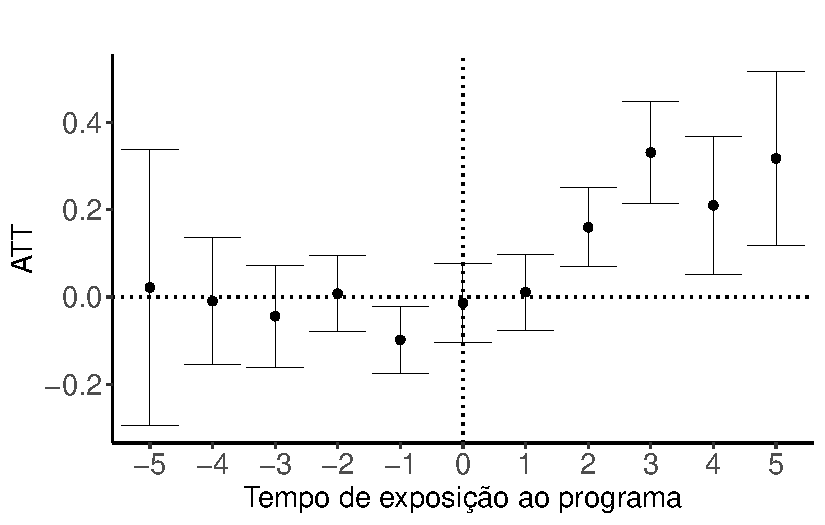
\includegraphics{script_files/figure-latex/unnamed-chunk-22-1.pdf}

\begin{Shaded}
\begin{Highlighting}[]
\NormalTok{plot\_did\_linguagem\_norm}
\end{Highlighting}
\end{Shaded}

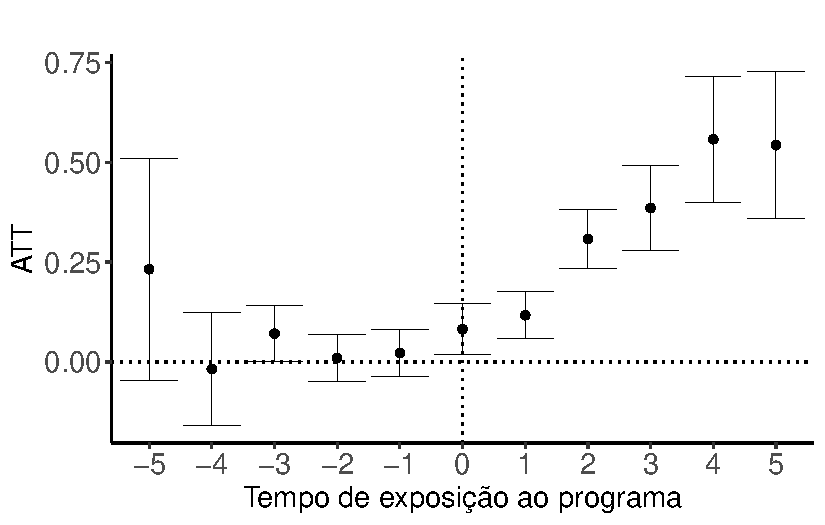
\includegraphics{script_files/figure-latex/unnamed-chunk-22-2.pdf}

\begin{Shaded}
\begin{Highlighting}[]
\NormalTok{plot\_did\_matematica\_norm}
\end{Highlighting}
\end{Shaded}

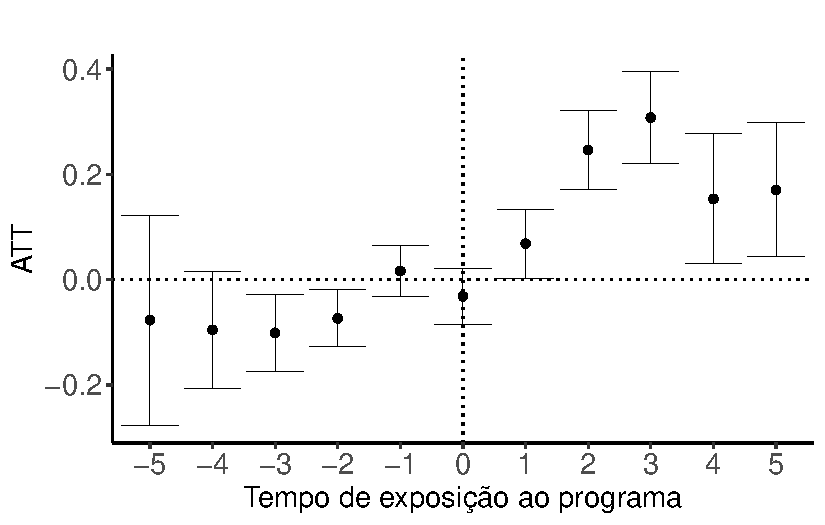
\includegraphics{script_files/figure-latex/unnamed-chunk-22-3.pdf}

\begin{Shaded}
\begin{Highlighting}[]
\NormalTok{plot\_did\_humanas\_norm}
\end{Highlighting}
\end{Shaded}

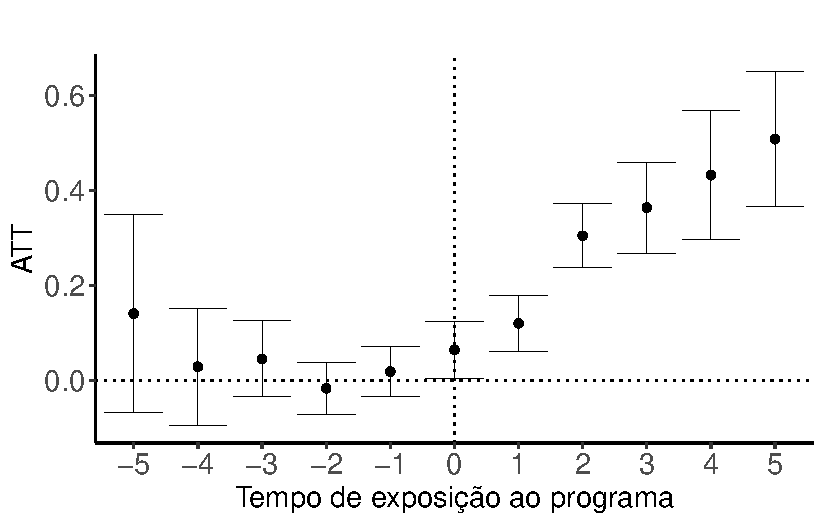
\includegraphics{script_files/figure-latex/unnamed-chunk-22-4.pdf}

\begin{Shaded}
\begin{Highlighting}[]
\NormalTok{plot\_did\_ciencias\_norm}
\end{Highlighting}
\end{Shaded}

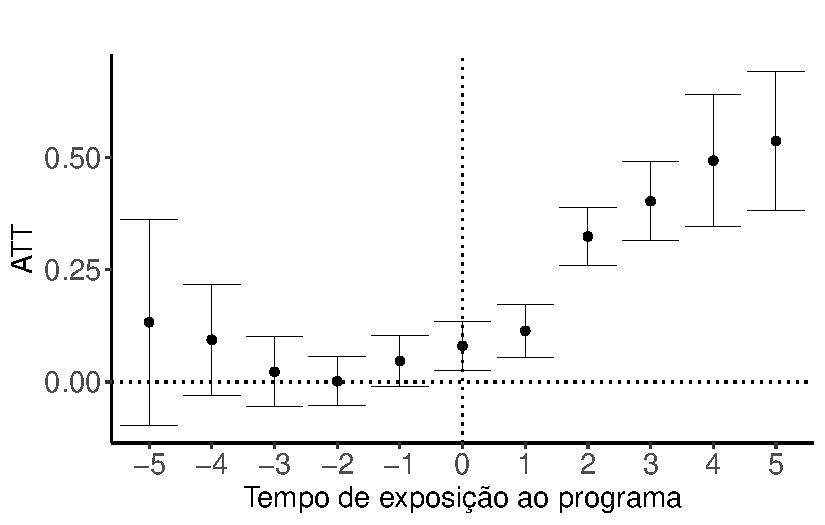
\includegraphics{script_files/figure-latex/unnamed-chunk-22-5.pdf}

\begin{Shaded}
\begin{Highlighting}[]
\NormalTok{plot\_did\_objetiva\_norm}
\end{Highlighting}
\end{Shaded}

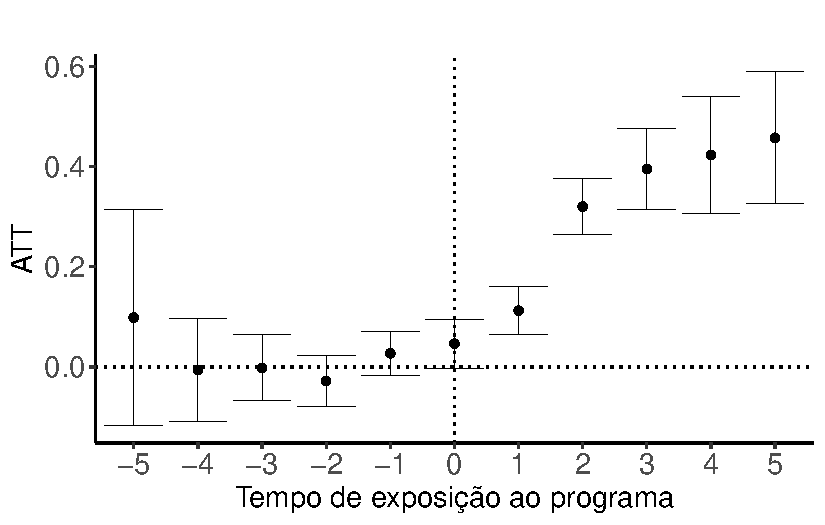
\includegraphics{script_files/figure-latex/unnamed-chunk-22-6.pdf}

\begin{Shaded}
\begin{Highlighting}[]
\NormalTok{plot\_did\_aprovacao\_norm }\OtherTok{\textless{}{-}}
\FunctionTok{ggdid}\NormalTok{(}\FunctionTok{aggte}\NormalTok{(did\_aprovacao\_norm, }\AttributeTok{type =} \StringTok{"dynamic"}\NormalTok{, }\AttributeTok{na.rm =}\NormalTok{ T),       }
      \AttributeTok{legend =}\NormalTok{ F, }\AttributeTok{ref\_line =} \DecValTok{0}\NormalTok{, }\AttributeTok{theming =}\NormalTok{ F)[[}\StringTok{"data"}\NormalTok{]] }\SpecialCharTok{\%\textgreater{}\%} 
    \FunctionTok{mutate}\NormalTok{(}\AttributeTok{ymin =}\NormalTok{ att}\SpecialCharTok{{-}}\NormalTok{c}\SpecialCharTok{*}\NormalTok{att.se, }\AttributeTok{ymax=}\NormalTok{att}\SpecialCharTok{+}\NormalTok{c}\SpecialCharTok{*}\NormalTok{att.se, }\AttributeTok{year=}\FunctionTok{as.factor}\NormalTok{(year)) }\SpecialCharTok{\%\textgreater{}\%} 
    \FunctionTok{ggplot}\NormalTok{(}\FunctionTok{aes}\NormalTok{(year, att)) }\SpecialCharTok{+}
    \FunctionTok{geom\_point}\NormalTok{(}\FunctionTok{aes}\NormalTok{(year, att)) }\SpecialCharTok{+}
    \FunctionTok{geom\_errorbar}\NormalTok{(}\FunctionTok{aes}\NormalTok{(}\AttributeTok{ymin =}\NormalTok{ ymin, }\AttributeTok{ymax =}\NormalTok{ ymax), }\AttributeTok{size =} \FloatTok{0.1}\NormalTok{) }\SpecialCharTok{+}
    \FunctionTok{labs}\NormalTok{(}\AttributeTok{title =} \StringTok{\textquotesingle{}\textquotesingle{}}\NormalTok{,}
         \AttributeTok{x =} \StringTok{\textquotesingle{}Tempo de exposição ao programa\textquotesingle{}}\NormalTok{,}
         \AttributeTok{y =}\StringTok{\textquotesingle{}ATT\textquotesingle{}}\NormalTok{) }\SpecialCharTok{+}
    \FunctionTok{geom\_vline}\NormalTok{(}\AttributeTok{xintercept =} \StringTok{\textquotesingle{}0\textquotesingle{}}\NormalTok{, }\AttributeTok{linetype =} \StringTok{\textquotesingle{}dotted\textquotesingle{}}\NormalTok{) }\SpecialCharTok{+}
    \FunctionTok{geom\_hline}\NormalTok{(}\AttributeTok{yintercept =} \DecValTok{0}\NormalTok{, }\AttributeTok{linetype =} \StringTok{\textquotesingle{}dotted\textquotesingle{}}\NormalTok{) }\SpecialCharTok{+}
\NormalTok{    tema\_did}

\FunctionTok{ggsave}\NormalTok{(plot\_did\_aprovacao\_norm, }
       \AttributeTok{filename =} \StringTok{"Plots/did\_agg\_aprovacao.pdf"}\NormalTok{,}
       \AttributeTok{device =} \StringTok{"pdf"}\NormalTok{,}
       \AttributeTok{width=}\FloatTok{7.5}\NormalTok{,}\AttributeTok{height=}\FloatTok{3.5}\NormalTok{, }\AttributeTok{units =} \StringTok{"in"}\NormalTok{)}

\NormalTok{plot\_did\_reprovacao\_norm }\OtherTok{\textless{}{-}}
\FunctionTok{ggdid}\NormalTok{(}\FunctionTok{aggte}\NormalTok{(did\_reprovacao\_norm, }\AttributeTok{type =} \StringTok{"dynamic"}\NormalTok{, }\AttributeTok{na.rm =}\NormalTok{ T),       }
      \AttributeTok{legend =}\NormalTok{ F, }\AttributeTok{ref\_line =} \DecValTok{0}\NormalTok{, }\AttributeTok{theming =}\NormalTok{ F)[[}\StringTok{"data"}\NormalTok{]] }\SpecialCharTok{\%\textgreater{}\%} 
    \FunctionTok{mutate}\NormalTok{(}\AttributeTok{ymin =}\NormalTok{ att}\SpecialCharTok{{-}}\NormalTok{c}\SpecialCharTok{*}\NormalTok{att.se, }\AttributeTok{ymax=}\NormalTok{att}\SpecialCharTok{+}\NormalTok{c}\SpecialCharTok{*}\NormalTok{att.se, }\AttributeTok{year=}\FunctionTok{as.factor}\NormalTok{(year)) }\SpecialCharTok{\%\textgreater{}\%} 
    \FunctionTok{ggplot}\NormalTok{(}\FunctionTok{aes}\NormalTok{(year, att)) }\SpecialCharTok{+}
    \FunctionTok{geom\_point}\NormalTok{(}\FunctionTok{aes}\NormalTok{(year, att)) }\SpecialCharTok{+}
    \FunctionTok{geom\_errorbar}\NormalTok{(}\FunctionTok{aes}\NormalTok{(}\AttributeTok{ymin =}\NormalTok{ ymin, }\AttributeTok{ymax =}\NormalTok{ ymax), }\AttributeTok{size =} \FloatTok{0.1}\NormalTok{) }\SpecialCharTok{+}
    \FunctionTok{labs}\NormalTok{(}\AttributeTok{title =} \StringTok{\textquotesingle{}\textquotesingle{}}\NormalTok{,}
         \AttributeTok{x =} \StringTok{\textquotesingle{}Tempo de exposição ao programa\textquotesingle{}}\NormalTok{,}
         \AttributeTok{y =}\StringTok{\textquotesingle{}ATT\textquotesingle{}}\NormalTok{) }\SpecialCharTok{+}
    \FunctionTok{geom\_vline}\NormalTok{(}\AttributeTok{xintercept =} \StringTok{\textquotesingle{}0\textquotesingle{}}\NormalTok{, }\AttributeTok{linetype =} \StringTok{\textquotesingle{}dotted\textquotesingle{}}\NormalTok{) }\SpecialCharTok{+}
    \FunctionTok{geom\_hline}\NormalTok{(}\AttributeTok{yintercept =} \DecValTok{0}\NormalTok{, }\AttributeTok{linetype =} \StringTok{\textquotesingle{}dotted\textquotesingle{}}\NormalTok{) }\SpecialCharTok{+}
\NormalTok{    tema\_did}

\FunctionTok{ggsave}\NormalTok{(plot\_did\_reprovacao\_norm, }
       \AttributeTok{filename =} \StringTok{"Plots/did\_agg\_reprovacao.pdf"}\NormalTok{,}
       \AttributeTok{device =} \StringTok{"pdf"}\NormalTok{,}
       \AttributeTok{width=}\FloatTok{7.5}\NormalTok{,}\AttributeTok{height=}\FloatTok{3.5}\NormalTok{, }\AttributeTok{units =} \StringTok{"in"}\NormalTok{)}

\NormalTok{plot\_did\_distorcao\_norm }\OtherTok{\textless{}{-}}
\FunctionTok{ggdid}\NormalTok{(}\FunctionTok{aggte}\NormalTok{(did\_distorcao\_norm, }\AttributeTok{type =} \StringTok{"dynamic"}\NormalTok{, }\AttributeTok{na.rm =}\NormalTok{ T),       }
      \AttributeTok{legend =}\NormalTok{ F, }\AttributeTok{ref\_line =} \DecValTok{0}\NormalTok{, }\AttributeTok{theming =}\NormalTok{ F)[[}\StringTok{"data"}\NormalTok{]] }\SpecialCharTok{\%\textgreater{}\%} 
    \FunctionTok{mutate}\NormalTok{(}\AttributeTok{ymin =}\NormalTok{ att}\SpecialCharTok{{-}}\NormalTok{c}\SpecialCharTok{*}\NormalTok{att.se, }\AttributeTok{ymax=}\NormalTok{att}\SpecialCharTok{+}\NormalTok{c}\SpecialCharTok{*}\NormalTok{att.se, }\AttributeTok{year=}\FunctionTok{as.factor}\NormalTok{(year)) }\SpecialCharTok{\%\textgreater{}\%} 
    \FunctionTok{ggplot}\NormalTok{(}\FunctionTok{aes}\NormalTok{(year, att)) }\SpecialCharTok{+}
    \FunctionTok{geom\_point}\NormalTok{(}\FunctionTok{aes}\NormalTok{(year, att)) }\SpecialCharTok{+}
    \FunctionTok{geom\_errorbar}\NormalTok{(}\FunctionTok{aes}\NormalTok{(}\AttributeTok{ymin =}\NormalTok{ ymin, }\AttributeTok{ymax =}\NormalTok{ ymax), }\AttributeTok{size =} \FloatTok{0.1}\NormalTok{) }\SpecialCharTok{+}
    \FunctionTok{labs}\NormalTok{(}\AttributeTok{title =} \StringTok{\textquotesingle{}\textquotesingle{}}\NormalTok{,}
         \AttributeTok{x =} \StringTok{\textquotesingle{}Tempo de exposição ao programa\textquotesingle{}}\NormalTok{,}
         \AttributeTok{y =}\StringTok{\textquotesingle{}ATT\textquotesingle{}}\NormalTok{) }\SpecialCharTok{+}
    \FunctionTok{geom\_vline}\NormalTok{(}\AttributeTok{xintercept =} \StringTok{\textquotesingle{}0\textquotesingle{}}\NormalTok{, }\AttributeTok{linetype =} \StringTok{\textquotesingle{}dotted\textquotesingle{}}\NormalTok{) }\SpecialCharTok{+}
    \FunctionTok{geom\_hline}\NormalTok{(}\AttributeTok{yintercept =} \DecValTok{0}\NormalTok{, }\AttributeTok{linetype =} \StringTok{\textquotesingle{}dotted\textquotesingle{}}\NormalTok{) }\SpecialCharTok{+}
\NormalTok{    tema\_did}

\FunctionTok{ggsave}\NormalTok{(plot\_did\_distorcao\_norm, }
       \AttributeTok{filename =} \StringTok{"Plots/did\_agg\_distorcao.pdf"}\NormalTok{,}
       \AttributeTok{device =} \StringTok{"pdf"}\NormalTok{,}
       \AttributeTok{width=}\FloatTok{7.5}\NormalTok{,}\AttributeTok{height=}\FloatTok{3.5}\NormalTok{, }\AttributeTok{units =} \StringTok{"in"}\NormalTok{)}

\NormalTok{plot\_did\_abandono\_norm }\OtherTok{\textless{}{-}}
\FunctionTok{ggdid}\NormalTok{(}\FunctionTok{aggte}\NormalTok{(did\_abandono\_norm, }\AttributeTok{type =} \StringTok{"dynamic"}\NormalTok{, }\AttributeTok{na.rm =}\NormalTok{ T),       }
      \AttributeTok{legend =}\NormalTok{ F, }\AttributeTok{ref\_line =} \DecValTok{0}\NormalTok{, }\AttributeTok{theming =}\NormalTok{ F)[[}\StringTok{"data"}\NormalTok{]] }\SpecialCharTok{\%\textgreater{}\%} 
    \FunctionTok{mutate}\NormalTok{(}\AttributeTok{ymin =}\NormalTok{ att}\SpecialCharTok{{-}}\NormalTok{c}\SpecialCharTok{*}\NormalTok{att.se, }\AttributeTok{ymax=}\NormalTok{att}\SpecialCharTok{+}\NormalTok{c}\SpecialCharTok{*}\NormalTok{att.se, }\AttributeTok{year=}\FunctionTok{as.factor}\NormalTok{(year)) }\SpecialCharTok{\%\textgreater{}\%} 
    \FunctionTok{ggplot}\NormalTok{(}\FunctionTok{aes}\NormalTok{(year, att)) }\SpecialCharTok{+}
    \FunctionTok{geom\_point}\NormalTok{(}\FunctionTok{aes}\NormalTok{(year, att)) }\SpecialCharTok{+}
    \FunctionTok{geom\_errorbar}\NormalTok{(}\FunctionTok{aes}\NormalTok{(}\AttributeTok{ymin =}\NormalTok{ ymin, }\AttributeTok{ymax =}\NormalTok{ ymax), }\AttributeTok{size =} \FloatTok{0.1}\NormalTok{) }\SpecialCharTok{+}
    \FunctionTok{labs}\NormalTok{(}\AttributeTok{title =} \StringTok{\textquotesingle{}\textquotesingle{}}\NormalTok{,}
         \AttributeTok{x =} \StringTok{\textquotesingle{}Tempo de exposição ao programa\textquotesingle{}}\NormalTok{,}
         \AttributeTok{y =}\StringTok{\textquotesingle{}ATT\textquotesingle{}}\NormalTok{) }\SpecialCharTok{+}
    \FunctionTok{geom\_vline}\NormalTok{(}\AttributeTok{xintercept =} \StringTok{\textquotesingle{}0\textquotesingle{}}\NormalTok{, }\AttributeTok{linetype =} \StringTok{\textquotesingle{}dotted\textquotesingle{}}\NormalTok{) }\SpecialCharTok{+}
    \FunctionTok{geom\_hline}\NormalTok{(}\AttributeTok{yintercept =} \DecValTok{0}\NormalTok{, }\AttributeTok{linetype =} \StringTok{\textquotesingle{}dotted\textquotesingle{}}\NormalTok{) }\SpecialCharTok{+}
\NormalTok{    tema\_did}

\FunctionTok{ggsave}\NormalTok{(plot\_did\_abandono\_norm, }
       \AttributeTok{filename =} \StringTok{"Plots/did\_agg\_abandono.pdf"}\NormalTok{,}
       \AttributeTok{device =} \StringTok{"pdf"}\NormalTok{,}
       \AttributeTok{width=}\FloatTok{7.5}\NormalTok{,}\AttributeTok{height=}\FloatTok{3.5}\NormalTok{, }\AttributeTok{units =} \StringTok{"in"}\NormalTok{)}
\end{Highlighting}
\end{Shaded}

\begin{Shaded}
\begin{Highlighting}[]
\NormalTok{plot\_did\_aprovacao\_norm}
\end{Highlighting}
\end{Shaded}

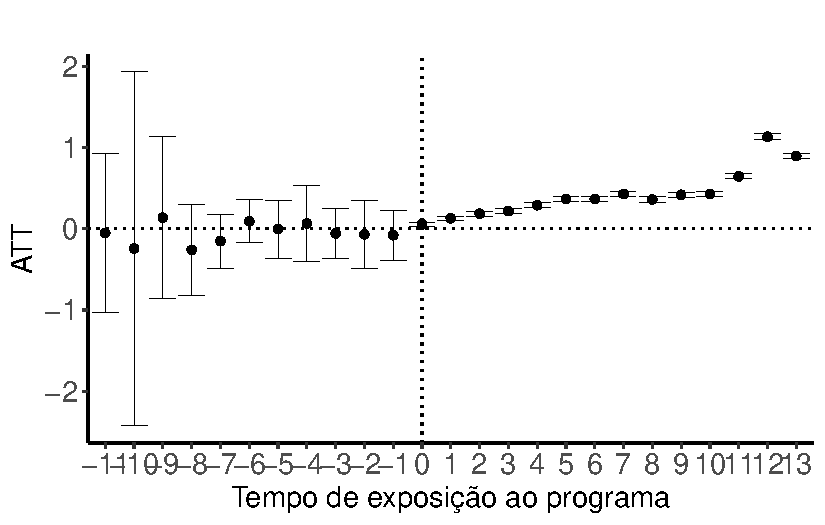
\includegraphics{script_files/figure-latex/unnamed-chunk-24-1.pdf}

\begin{Shaded}
\begin{Highlighting}[]
\NormalTok{plot\_did\_reprovacao\_norm}
\end{Highlighting}
\end{Shaded}

\includegraphics{script_files/figure-latex/unnamed-chunk-24-2.pdf}

\begin{Shaded}
\begin{Highlighting}[]
\NormalTok{plot\_did\_distorcao\_norm}
\end{Highlighting}
\end{Shaded}

\includegraphics{script_files/figure-latex/unnamed-chunk-24-3.pdf}

\begin{Shaded}
\begin{Highlighting}[]
\NormalTok{plot\_did\_abandono\_norm}
\end{Highlighting}
\end{Shaded}

\includegraphics{script_files/figure-latex/unnamed-chunk-24-4.pdf}



\end{document}
